\documentclass{beamer}
\usepackage{amsmath}
\usepackage{amssymb}
\usepackage{graphicx}
%\usetheme[height=7mm]{Rochester}
%\usepackage{beamerthemesplit}
\usepackage{algorithm}
\usepackage{algorithmic}
% Loading of sagetex for my inline sage code
\usepackage{sagetex}
\usepackage{url}


\usetheme{Pittsburgh}

\newtheorem{proposition}[theorem]{Proposition}


% Options and loading of xypic for diagrams
\usepackage[all]{xy}
\SelectTips{cm}{}
%\CompileMatrices
\entrymodifiers={+!!<0pt,\fontdimen22\textfont2>}


% Define special graph operators

\newcommand{\zigzag}{\mathbin{\raisebox{.2ex}{
      \hspace{-.4em}$\bigcirc$\hspace{-.75em}{\rm z}\hspace{.25em}}}}
\newcommand{\sandwich}{\mathbin{\raisebox{.2ex}{
      \hspace{-.4em}$\bigcirc$\hspace{-.75em}{\rm s}\hspace{.25em}}}}
\newcommand{\concat}{\mathbin{\raisebox{.2ex}{
      \hspace{-.4em}$\bigcirc$\hspace{-.75em}{\rm c}\hspace{.25em}}}}
\newcommand{\zig}{\mathbin{\raisebox{.2ex}{
      \hspace{-.4em}$\bigcirc$\hspace{-.75em}{\rm i}\hspace{.25em}}}}
\newcommand{\zag}{\mathbin{\raisebox{.2ex}{
      \hspace{-.4em}$\bigcirc$\hspace{-.75em}{\rm a}\hspace{.25em}}}}
\newcommand{\replacement}{\mathbin{\raisebox{.2ex}{
      \hspace{-.4em}$\bigcirc$\hspace{-.65em}{\rm r}}\hspace{.35em}}}





% Other useful packages for theses (see LaTeX docs for descriptions of these)
%\usepackage{varioref} % for the \vref commands that also prints out the reference page
%\usepackage{alltt} % for including computer code

\usepackage{url} % for the \url{http://foo.com} command to include url's (or filenames)
%\usepackage{longtable} % For multi page tables

% The style of theorems and such that you want to use.  You can change the
% style by modifying the second argument (for example prepending '\sc ' as
% in {\sc Theorem} which will make the headings come out as small caps rather
% then bold)

% \newtheorem{theorem}{Theorem}[section]
% \newtheorem{lemma}[theorem]{Lemma}
% \newtheorem{corollary}[theorem]{Corollary}
% \newtheorem{proposition}[theorem]{Proposition}

% \theoremstyle{definition}
% \newtheorem{definition}[theorem]{Definition}
% \newtheorem{example}[theorem]{Example}

% \theoremstyle{remark}
% \newtheorem{remark}[theorem]{Remark}


% Declaring Math operators that are used in the paper
\DeclareMathOperator{\Set}{\mathrm{\mathbf{Set}}}
\DeclareMathOperator{\Top}{\mathrm{\mathbf{Top}}}
\DeclareMathOperator{\Net}{\mathrm{\mathbf{Net}}}
\DeclareMathOperator{\SymNet}{\mathbf{SymNet}}
\DeclareMathOperator{\Grp}{\mathbf{Grp}}
\DeclareMathOperator{\Isop}{\mathrm{i}}
\DeclareMathOperator{\Aut}{\mathrm{Aut}}
\DeclareMathOperator{\id}{\mathrm{id}}
\DeclareMathOperator{\inv}{\mathrm{inv}}
\DeclareMathOperator{\Act}{\mathrm{\phi}}
\DeclareMathOperator{\Orb}{\mathrm{\Phi}}
\DeclareMathOperator{\Stab}{\mathrm{stab}}
\DeclareMathOperator{\CG}{\mathrm{C}}
\DeclareMathOperator{\Term}{\mathbf{\tau}}
\DeclareMathOperator{\Source}{\mathbf{\varsigma}}
\DeclareMathOperator{\Rot}{\mathbf{\varrho}}

\DeclareMathOperator{\enum}{\eta}
\DeclareMathOperator{\Enum}{\mathcal{E}}
\DeclareMathOperator{\EnumSet}{\mathbf{E}}

\DeclareMathOperator{\ppath}{\mathit{p}}
\DeclareMathOperator{\cpath}{\mathit{c}}
\DeclareMathOperator{\pcd}{\mathcal{D}}
\DeclareMathOperator{\pcdSet}{\mathbf{P}}


\DeclareMathOperator{\trellis}{\mathbb{T}}





%% Group action macros

\newcommand{\acts}[2]{\ensuremath{#1 \cdot #2}}
\newcommand{\orbit}[2]{ \ensuremath{\Orb_{#1}\left(#2 \right)}}
\newcommand{\stab}[2]{\ensuremath{\Stab_{#1}\left(#2 \right)}} 
\newcommand{\card}[1]{\ensuremath{\left\vert #1 \right\vert}}
\newcommand{\cg}[2]{\ensuremath{\CG(#1,#2)}}
\newcommand{\cn}[2]{\ensuremath{\CG(#1,#2)}}



\newcommand{\rot}[1]{\ensuremath{\overline{#1}}}
\newcommand{\source}[1]{\ensuremath{\Source\left(#1\right)}}
\newcommand{\term}[1]{\ensuremath{\Term\left(#1\right)}}


\newcommand{\edgeS}[1]{\ensuremath{\mathrm{E}(#1) }}
\newcommand{\edgeSet}[1]{\ensuremath{\mathrm{E}\left( #1 \right)}}


\newcommand{\edgeG}{\ensuremath{\mathrm{E}}}
\newcommand{\edgeH}{\ensuremath{\mathrm{F}}}



\newcommand{\vertS}[1]{\ensuremath{\mathrm{V}(#1)}}
\newcommand{\vertG}{\ensuremath{\mathrm{V}}}
\newcommand{\vertH}{\ensuremath{\mathrm{W}}}

\newcommand{\symnet}[3]{\ensuremath{ #1: \left( \rot{#2} , #3 \right)}}
\newcommand{\net}[3]{\ensuremath{#1:\left(#2,#3\right)}}




\title{EXPANDING FAMILIES, THE ZIG-ZAG AND REPLACEMENT PRODUCTS}
\subtitle{A Thesis Presented to the Faculty of San Diego State University}
\author{David M. Monarres \\ Candidate for Masters of Arts, Pure Mathematics \\dmmonarres@gmail.com}
\date{Tuesday, May 17, 2011}

\begin{document}

\frame{\titlepage}

\part{Introduction}

\begin{frame}{Purpose of Thesis}
\centering
\only<2>{{\Huge \alert{TO FINISH!}}}
  
\end{frame}

\begin{frame}{Purpose of Thesis}
\begin{block}{Three Objects:}
\begin{itemize} 
\item<2->{\em Zig-Zag} Graph Product.
\item<3-> {\em Replacement} Graph Product.
\item<4-> {\em Enumerations} that generate them.
\end{itemize}
\end{block}

\begin{center}
\uncover<2->{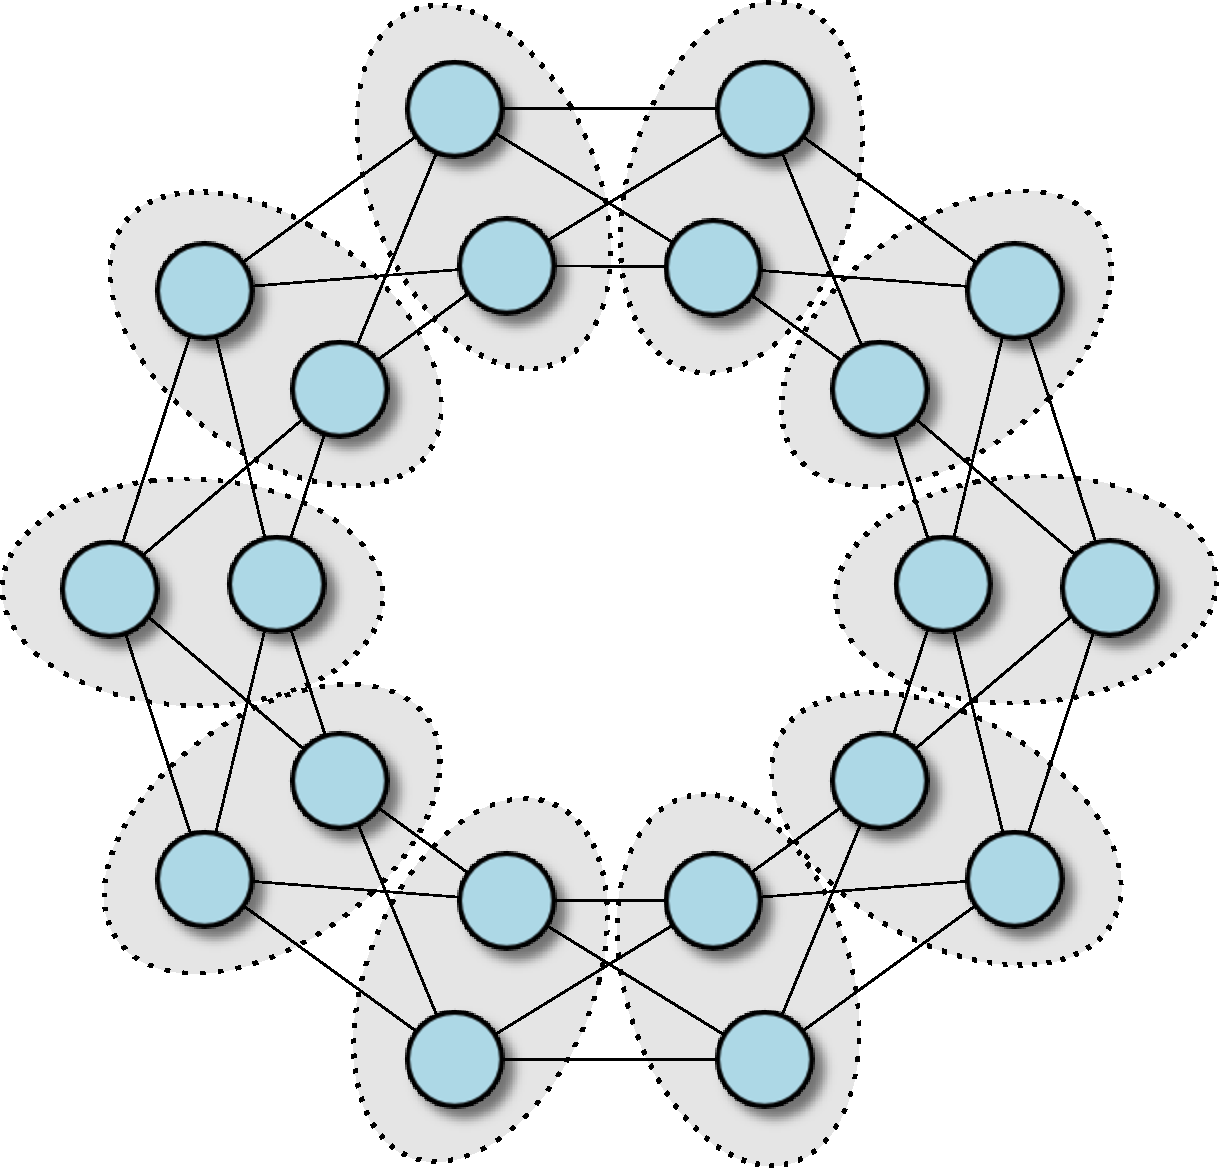
\includegraphics[height=.33\textheight]{../pics/10-zigzag}}\hspace*{2em}
\uncover<3->{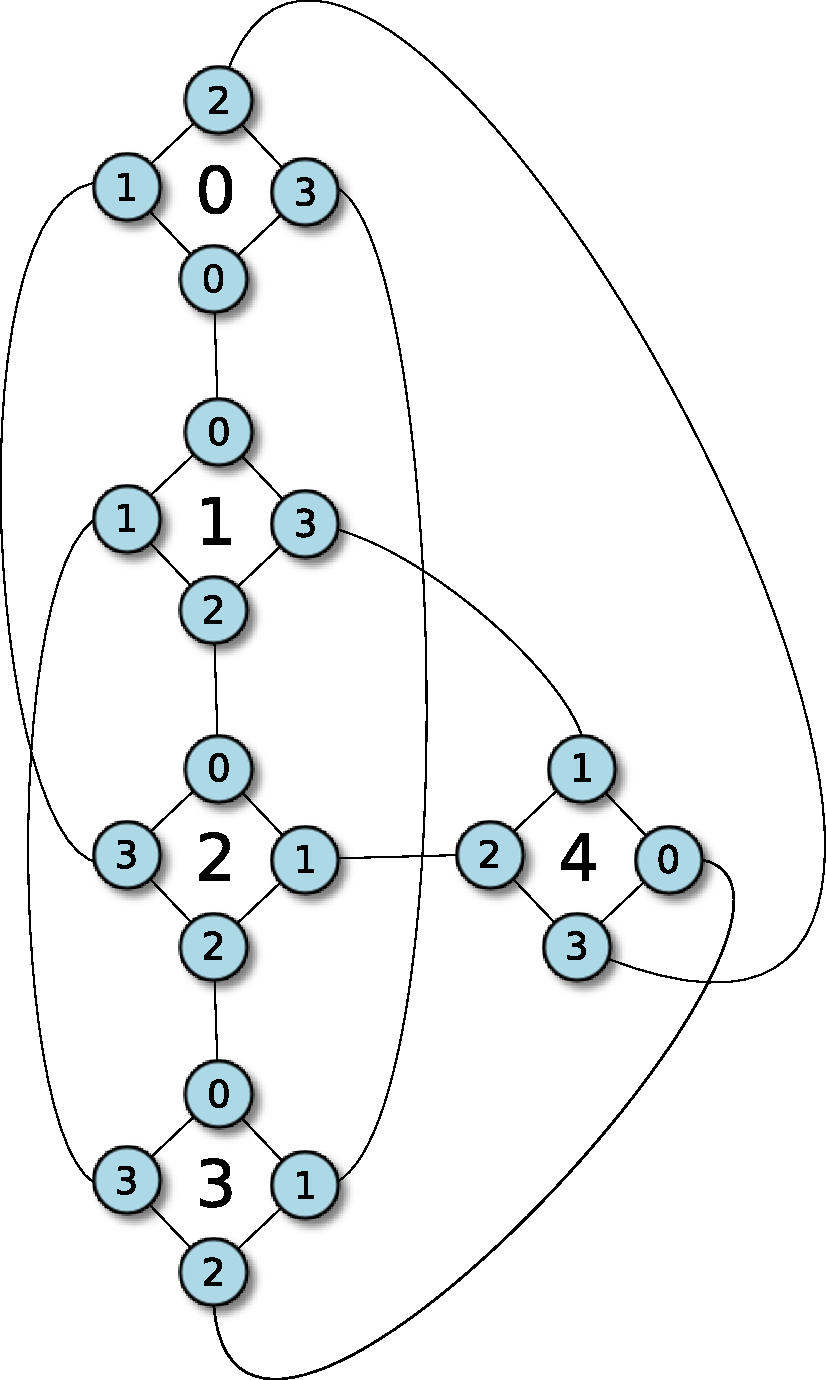
\includegraphics[height=.33\textheight]{../pics/10_5d8s-replacement-0123420314}}\hspace*{2em}
\uncover<4->{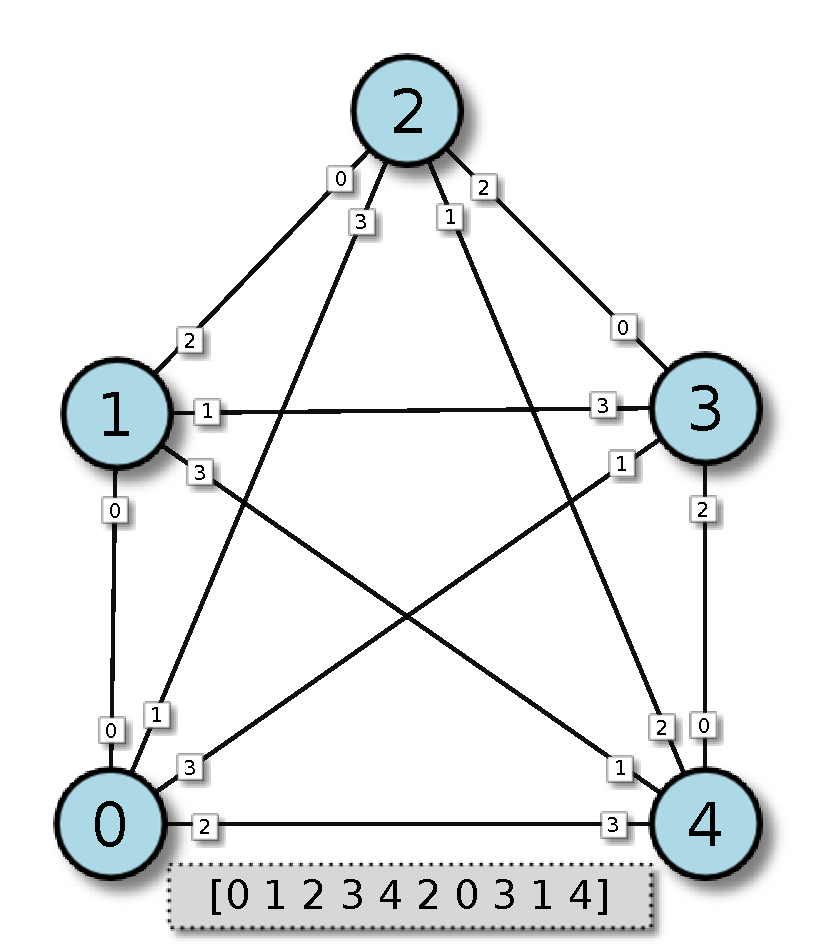
\includegraphics[height=.33\textheight]{../pics/K5-10_5d8s-0123420314}}
\end{center}
\end{frame}


\begin{frame}{History}
\centering
  \begin{columns}
  \column{.50\textwidth}
  \begin{block}{The Zig-Zag Product}
    \begin{itemize}
    \item<2-> Developed by {Reingold, Vadhan and Widgerson}~\cite{Reingold:2002ys} in 2000.
    \item<3-> Principally to facilitate the explicit construction of graphs with good {\em expansion} properties.
    \end{itemize}
  \end{block}
  \column{.50\textwidth}
  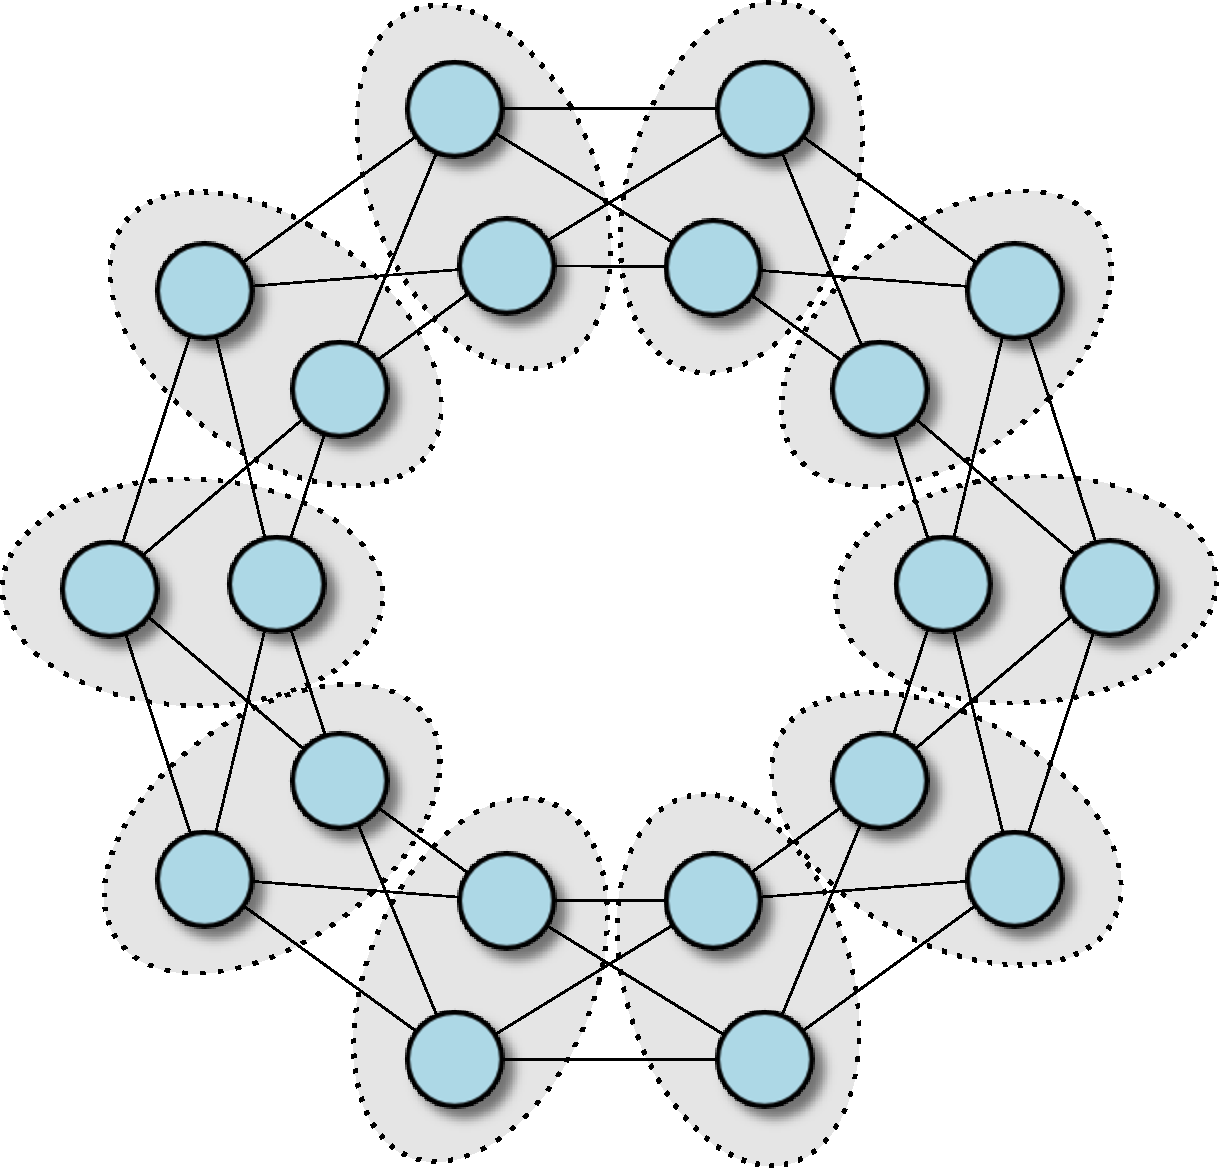
\includegraphics[width=.70\textwidth]{../pics/10-zigzag}
  \end{columns}
\end{frame}

\begin{frame}{History:}

    \begin{block}{What is {\em expansion}?}
      \begin{itemize}
      \item<2-> A graph with good expansion properties, roughly speaking, is a graph that is {\em robustly} connected.  
      \end{itemize}
    \end{block}
    \begin{block}{What are {\em expander graphs} good for?}<3->
      They have been used in fields such as:
      \begin{itemize}
        \item<4-> Network Design~\cite{Pippenger:1982nx, Nicholas-Pippenger:1987eu}
        \item<5-> Complexity Theory~\cite{Urquhart:1987cr,Valiant:1977dq}
        \item<6-> Topology~\cite{MR1826251} and Measure Theory~\cite{Lubotzky:1994ve}
      \end{itemize}
    \end{block}
\end{frame}

\section{Measuring Expansion} 

\begin{frame}{How do we measure expansion?}


 \begin{definition}
The {\bf edge boundary} of $S \subseteq V$ is the set $\partial S \subseteq E$ defined to be: 
\[  \partial S = \left\{ \left(u,v\right) \ \vert \ u \in S \ {\rm and }\  v \in V - S     \right\}  \]
\label{def:edge_boundary}
\end{definition}
\begin{figure}[h]
  \centering
  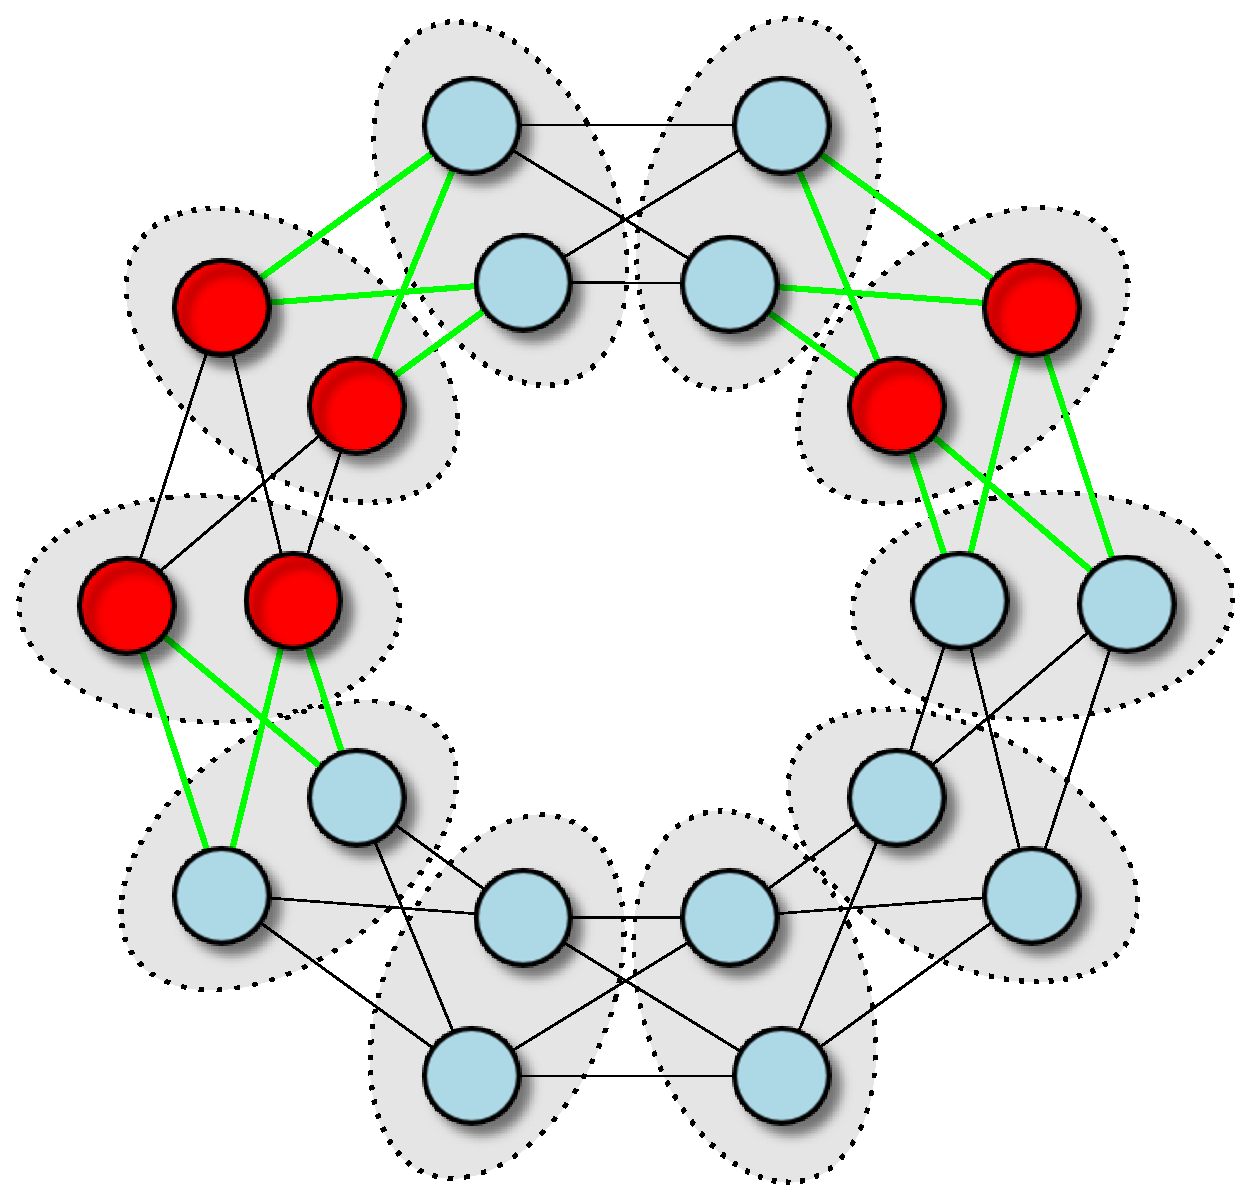
\includegraphics[height=.40\textheight]{../pics/edge_boundary}
  \caption{Example $\partial S $ for $2$-trellis over $C_10$}
  \label{fig:edgeboundary}
\end{figure}
\end{frame}

\begin{frame}{How do we measure expansion?}
\begin{definition}
\label{def:isoperimetric_measure}
Let $G$ be a graph and $S \subseteq V(G)$. The {\bf isoperimetric constant}  of $G$ is
\[ 
i(G) =  \inf_{ \stackrel{S \subseteq V}{0 <  \left| S \right| < \infty   } } \frac{\left|\partial S\right| }{ \min\left\{ \left|S \right|, \left|V - S\right|   \right\} }
\]
\end{definition}
\begin{figure}[h]
  \centering
  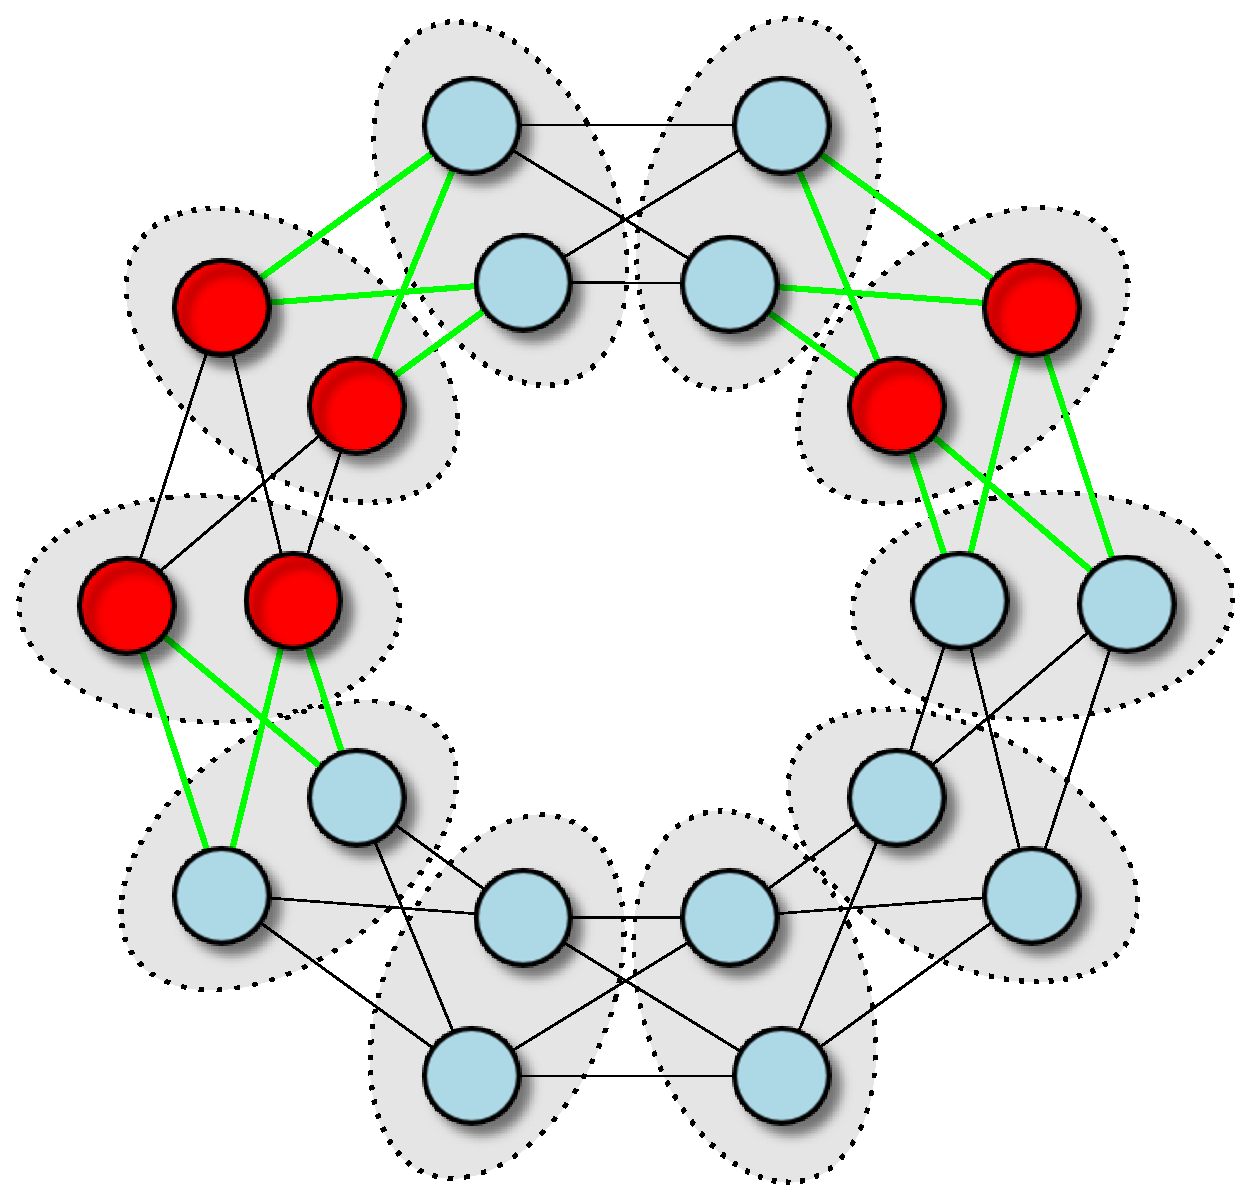
\includegraphics[height=.40\textheight]{../pics/edge_boundary}
  \caption{Example $\partial S $ for $2$-trellis over $C_10$}
  \label{fig:edgeboundary}
\end{figure}
\end{frame}

\begin{frame}{Examples}

  \begin{columns}
    \column{.50\textwidth}
    \only<1>{
      \begin{example}{Disconnected Graph, $G$}
         \[ i(G) = 0. \] 
         Since $\partial S = \emptyset$ for any {\em component} $S$. 
       \end{example}}
    \only<2>{
      \begin{example}<2->{Cycle Graph, $C_n$}
        \[ i(G) = \frac{2}{ \left\lfloor \frac{n}{2} \right\rfloor}\]
        Since every chain of length $m$ has a boundary of size 2. 
      \end{example}
    }
    \only<3>{
    \begin{example}<3->{The Complete Graph, $K_n$}
      \[ i(G) =  n - \left\lfloor \frac{n}{2} \right\rfloor = \left\lceil \frac{n}{2} \right\rceil. \] Since for all $S \subset \vertS{K_n}$, $\card{\partial S} = m\left(n-m\right)$
    \end{example}
    }
    \column{.50\textwidth}
    \only<1>{
      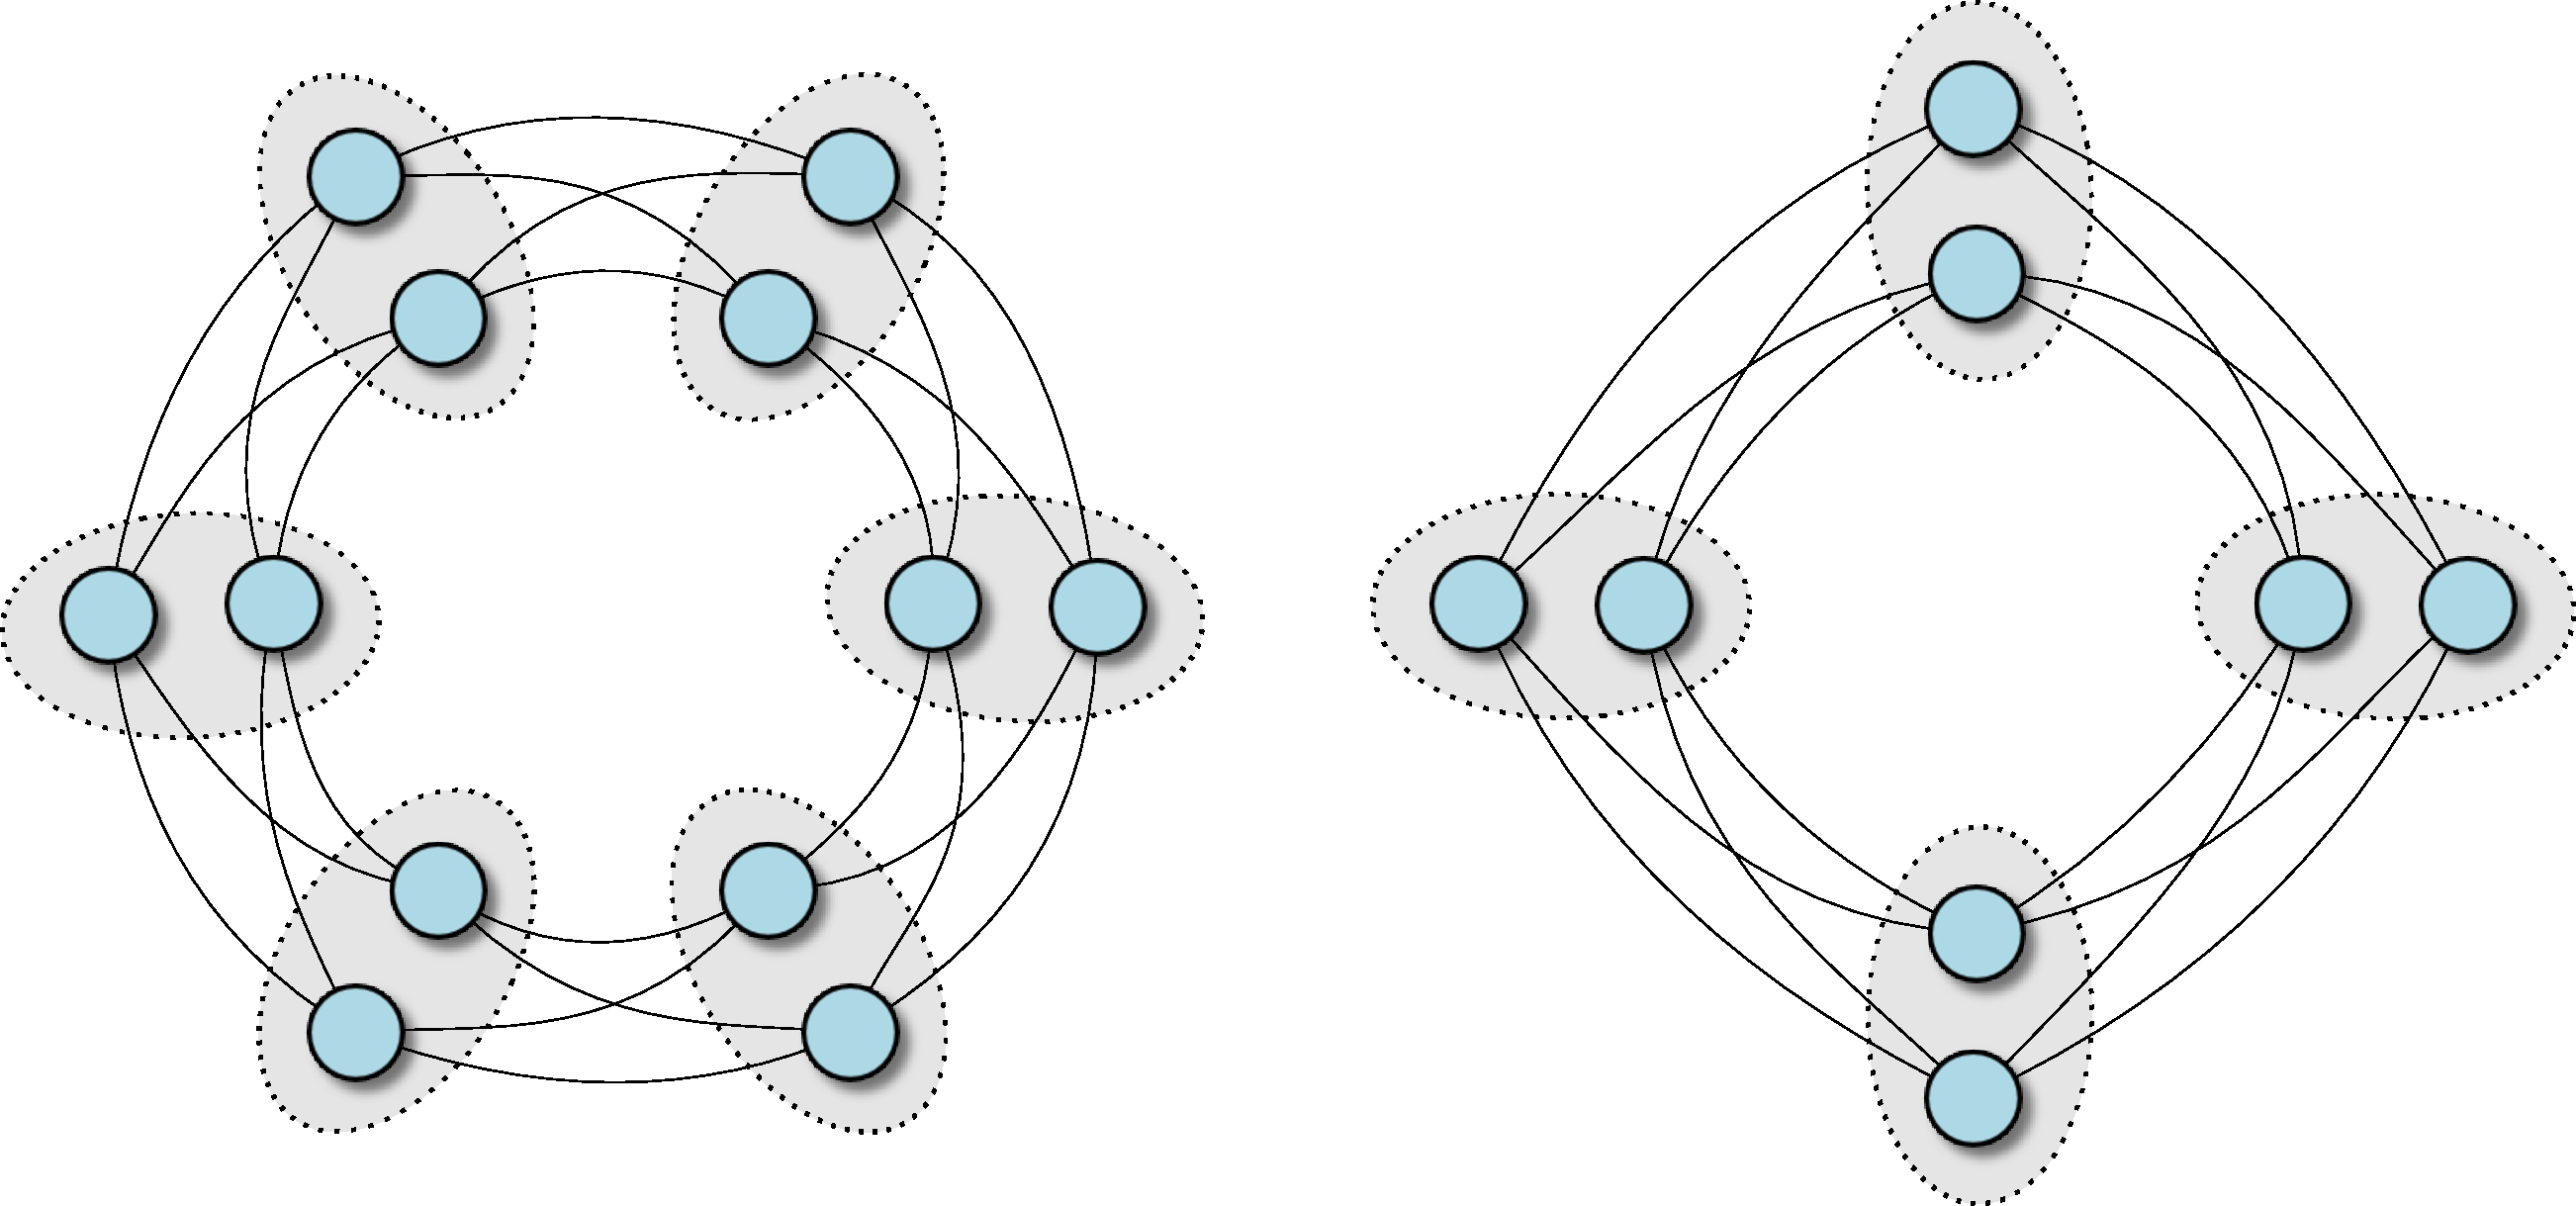
\includegraphics[width=.90\textwidth]{../pics/4-6-zigzag}
    }
    \only<2>{
      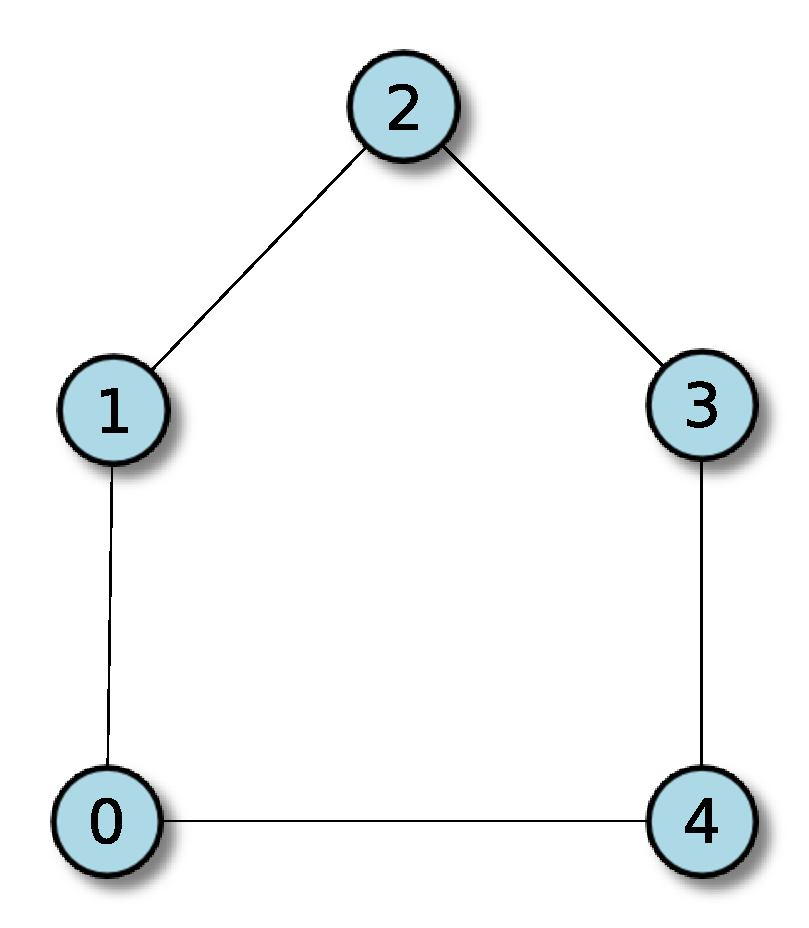
\includegraphics[width=.90\textwidth]{../pics/C5}
    }
    \only<3>{
      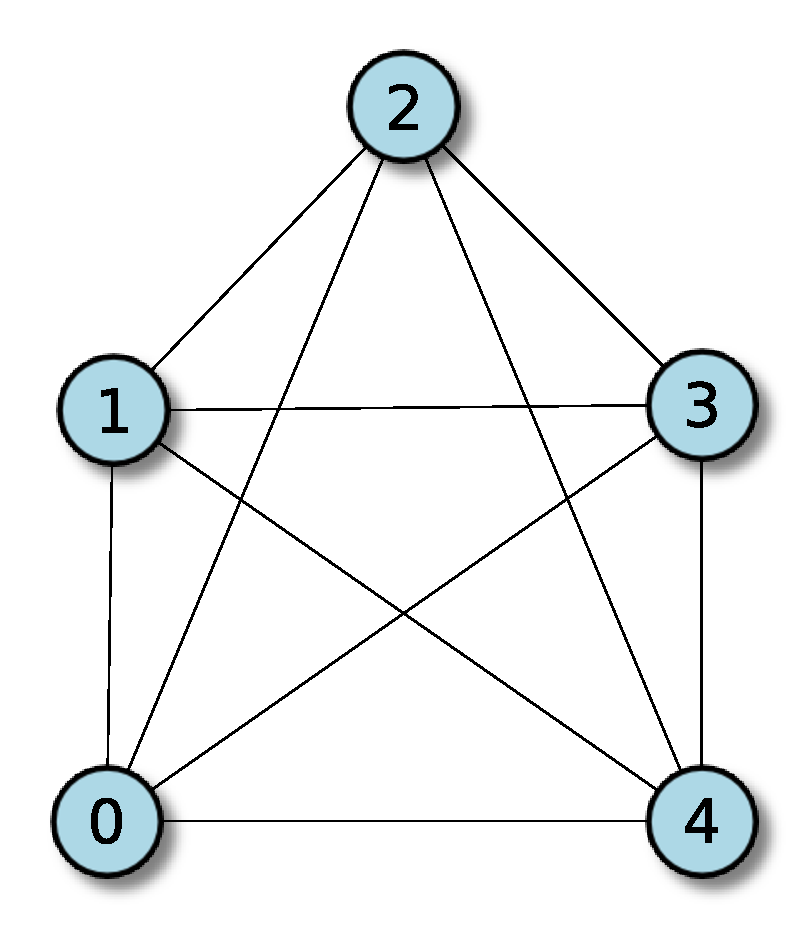
\includegraphics[width=.90\textwidth]{../pics/K5plain}
    }
  \end{columns}
  
\end{frame}

\begin{frame}{Expanding Families of Graphs}
\begin{definition}
  \label{def:expanding_family}
Let $\mathcal{F} = \left\{ G_k \ \vert \ k \in \mathbb{N} \right\}$ be a collection of graphs with $\card{\vertS{G_k}} = n_k$  and $n_k \rightarrow \infty$ as $k \rightarrow \infty$. $\mathcal{F}$ is called an {\bf expanding family } of graphs if 
\begin{itemize}
\item There exists an $\epsilon > 0 $ such that $ \epsilon \leq i\left( G_k \right)$ for all $G_k \in \mathcal{F}$.
\end{itemize} 
\end{definition}

\begin{block}<2->{}
Each $G_k \in \mathcal{F}$ is known as an {\bf $\epsilon$-expander graph} or sometimes just an {\bf expander}.
\end{block}
  
\begin{columns}
  \column{.50\textwidth}
  \begin{example}<3->{ $\mathcal{C} = \left\{ C_n\ \vert\ n \in \mathbb{N} \right\}$ } 
    \[ \lim_{n \rightarrow \infty} \frac{2}{ \left\lfloor \frac{n}{2} \right\rfloor} = 0        \]
  \end{example}
  \column{.50\textwidth}
  \begin{example}<4->{$ \mathcal{K} =  \left\{ K_n\ \vert\ n \in \mathbb{N} \right\}$}
   \[ \lim_{n \rightarrow \infty}  \left\lceil \frac{n}{2} \right\rceil = \infty  \] 
  \end{example}
\end{columns}

\end{frame}

\begin{frame}{Spectral Measure of Expansion}

  \begin{block}{Spectrum of a Regular Undirected Graph}
    Let $G$ is a $d$-regular undirected graph on $n$ vertices. Then $A(G)$ is a real and symmetric matrix, and thus has real eigenvalues which can be placed in descending order \[ d = \lambda_{1} \geq \lambda_{2} \geq \cdots \geq \lambda_{n-1} \geq \lambda_{n} \]  
  \end{block}

\begin{theorem}<2->
\[ \frac{d - \lambda_2  }{ 2} \leq  i(G)  \leq \sqrt{2d \left(d - \lambda_2 \right) }  \] 
\label{thm:spectral_expansion}
\end{theorem}
\uncover<3->{{\small Many times the {\em normalized adjacency matrix}, $\hat{A}(G) = \frac{1}{d} A(G)$ is used and expansion is measured in terms of convergence of a {\em random walk} on $G$.}}
\end{frame}


\begin{frame}{Expansion and the Zig-Zag Product}
\begin{theorem}
\label{thm:zigzag}
\noindent
Let $G$ be a $m$-regular graph on $n$ vertices and let $H$ be a $d$-regular graph on $m$ vertices and let $\alpha, \beta$ be such that $\hat{\lambda}_2(G) \leq \alpha$ and $\hat{\lambda}_2(H) \leq \beta$. Then $G \zigzag H$ is a $d^2$-regular graph on $n\cdot m$ vertices where the function $\hat{\lambda}_{2}(G \zigzag H)$ satisfies the following:
\begin{itemize}
\item If $\alpha < 1$  and $\beta < 1$ then $\hat{\lambda}_{2}(G \zigzag H) < 1$.
\item  $\hat{\lambda}_{2}(G \zigzag H) \leq \alpha + \beta$.
\end{itemize}
\end{theorem}
      \begin{figure}[h]
      \centering
          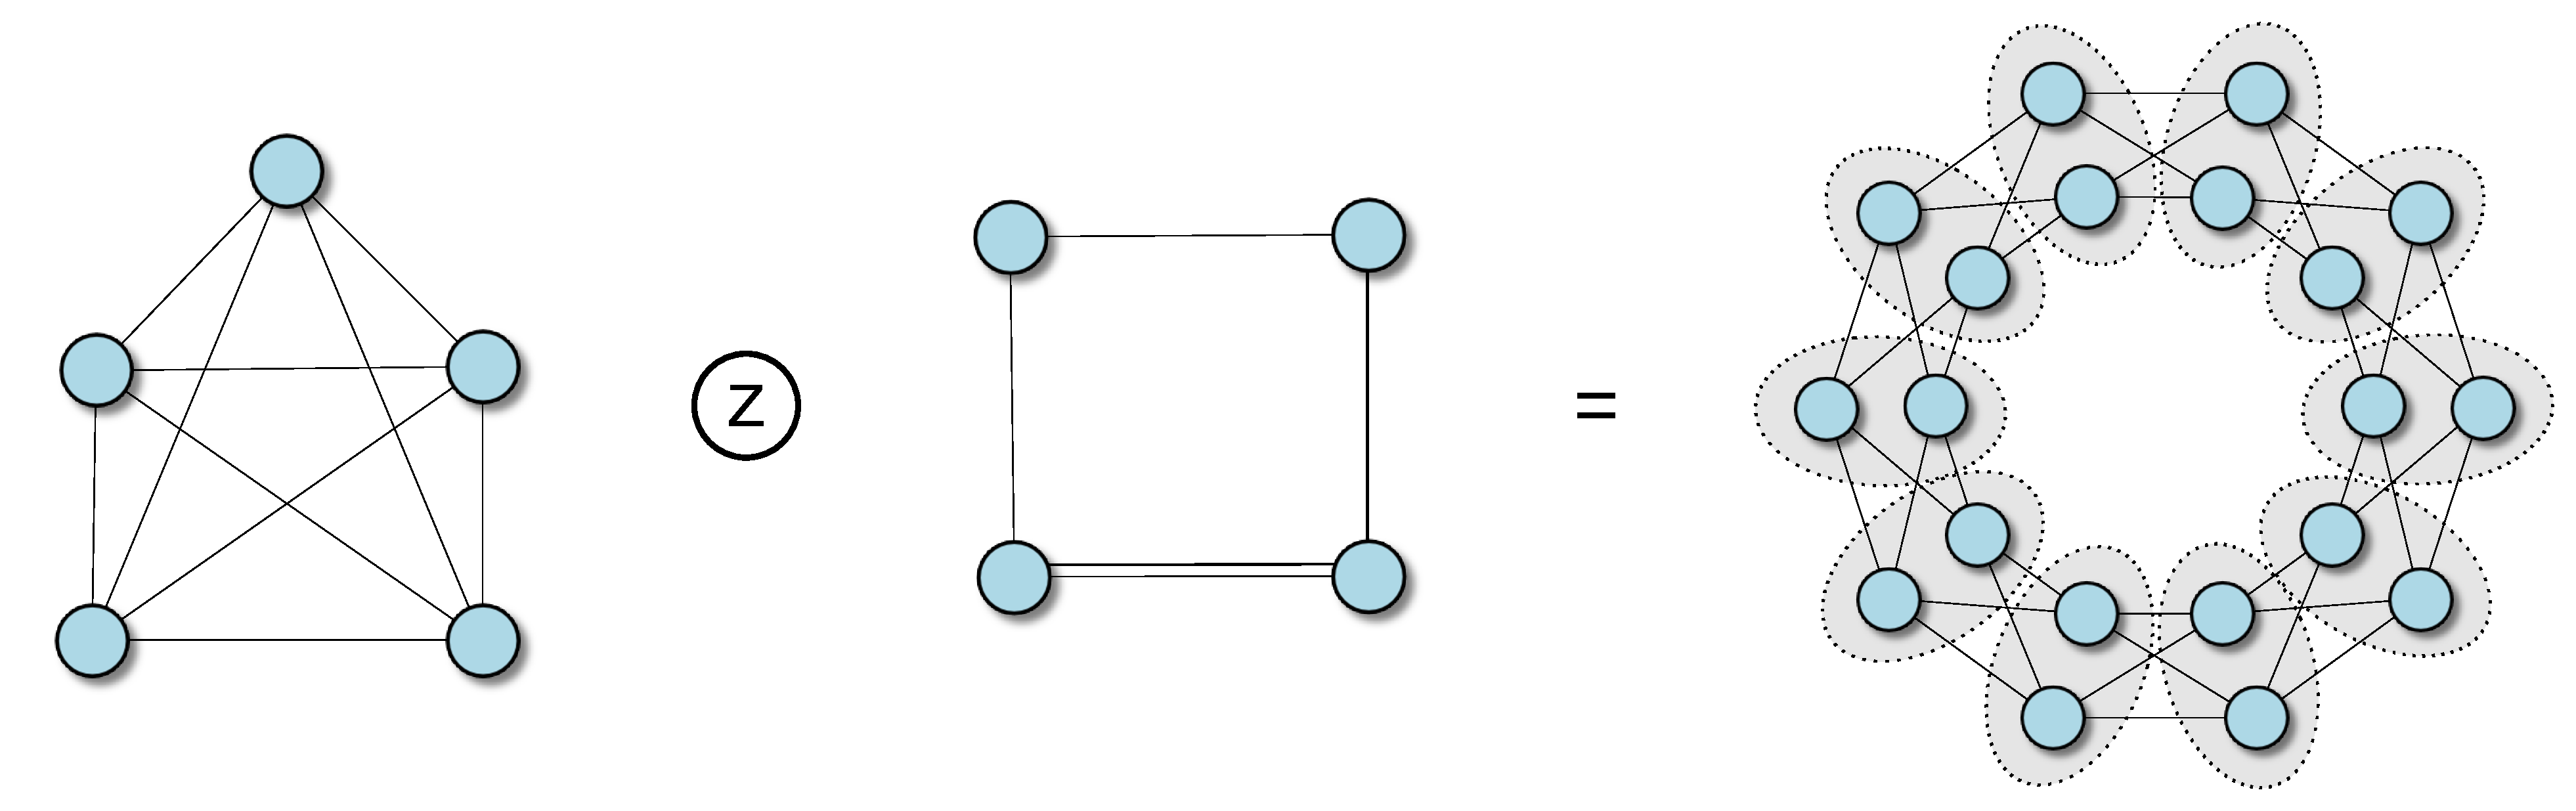
\includegraphics[width=.90\textwidth]{../pics/zigzag-example-generic}
      \caption{Generic Example of Zig-Zag Product}
    \end{figure}
\end{frame}


\begin{frame}{Expansion and the Zig-Zag Product}
  \begin{block}{What does the last theorem prove?} 
   If $G$ and $H$ have good expansion then $G \zigzag H$ does also.
  \end{block}
  \begin{center}
    \begin{figure}[h]
      \centering
          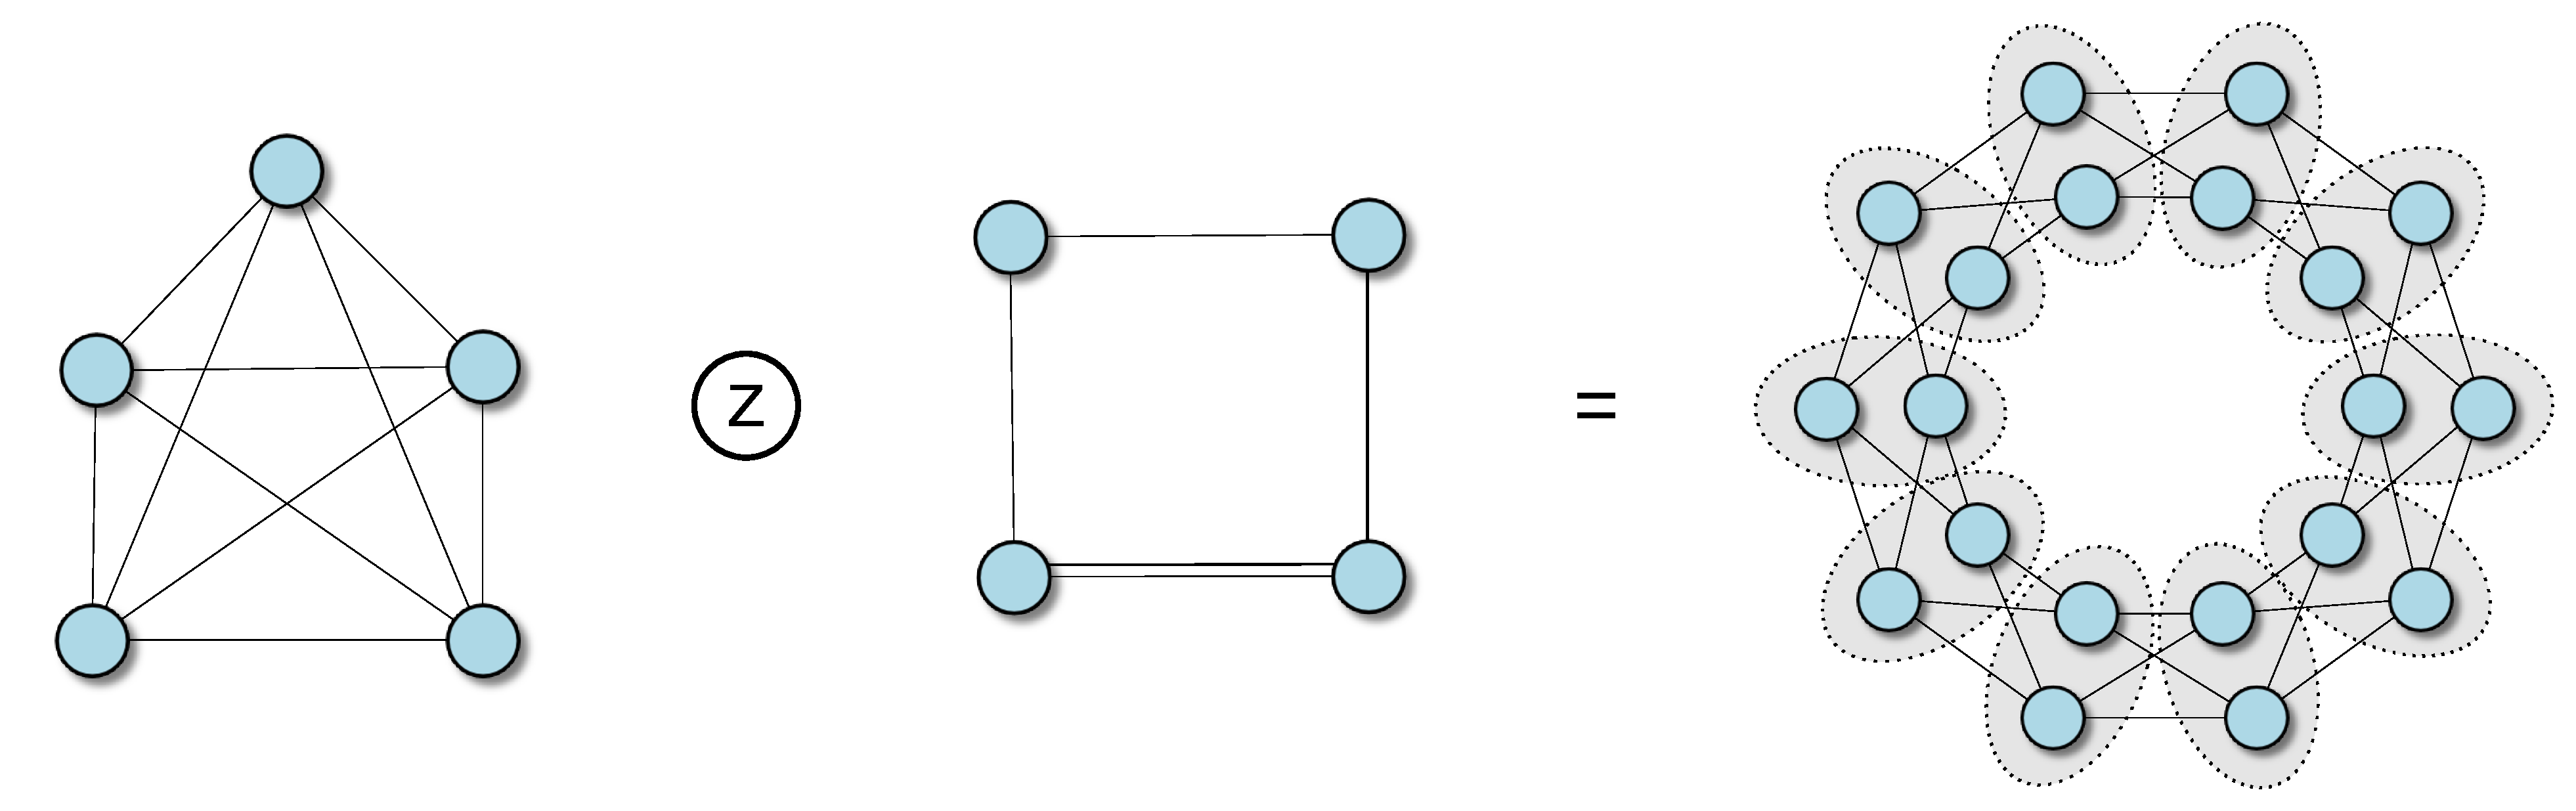
\includegraphics[width=.88\textwidth]{../pics/zigzag-example-generic}
      \caption{Generic Example of Zig-Zag Product}
    \end{figure}
  \end{center}
  \begin{block}{Why?}
   Guarantees that the {\em spectral gap} is bounded away from $0$.
  \end{block}
\end{frame}

\begin{frame}{But, I have left something out.}
  \begin{block}{}
    \begin{itemize}
    \item<1->  When we speak of \alert{the} zig-zag product of $G$ and $H$ we, and much of the literature, have left out an important detail.
    \item<2-> Even with two fixed constituent graphs there are really \alert{many} zig-zag products, some of which are non-isomorphic. 
    \end{itemize}
  \end{block}  

  \begin{block}<3->{Example of three different  $K_5 \zigzag C_4$}
    \begin{center}
    \framebox{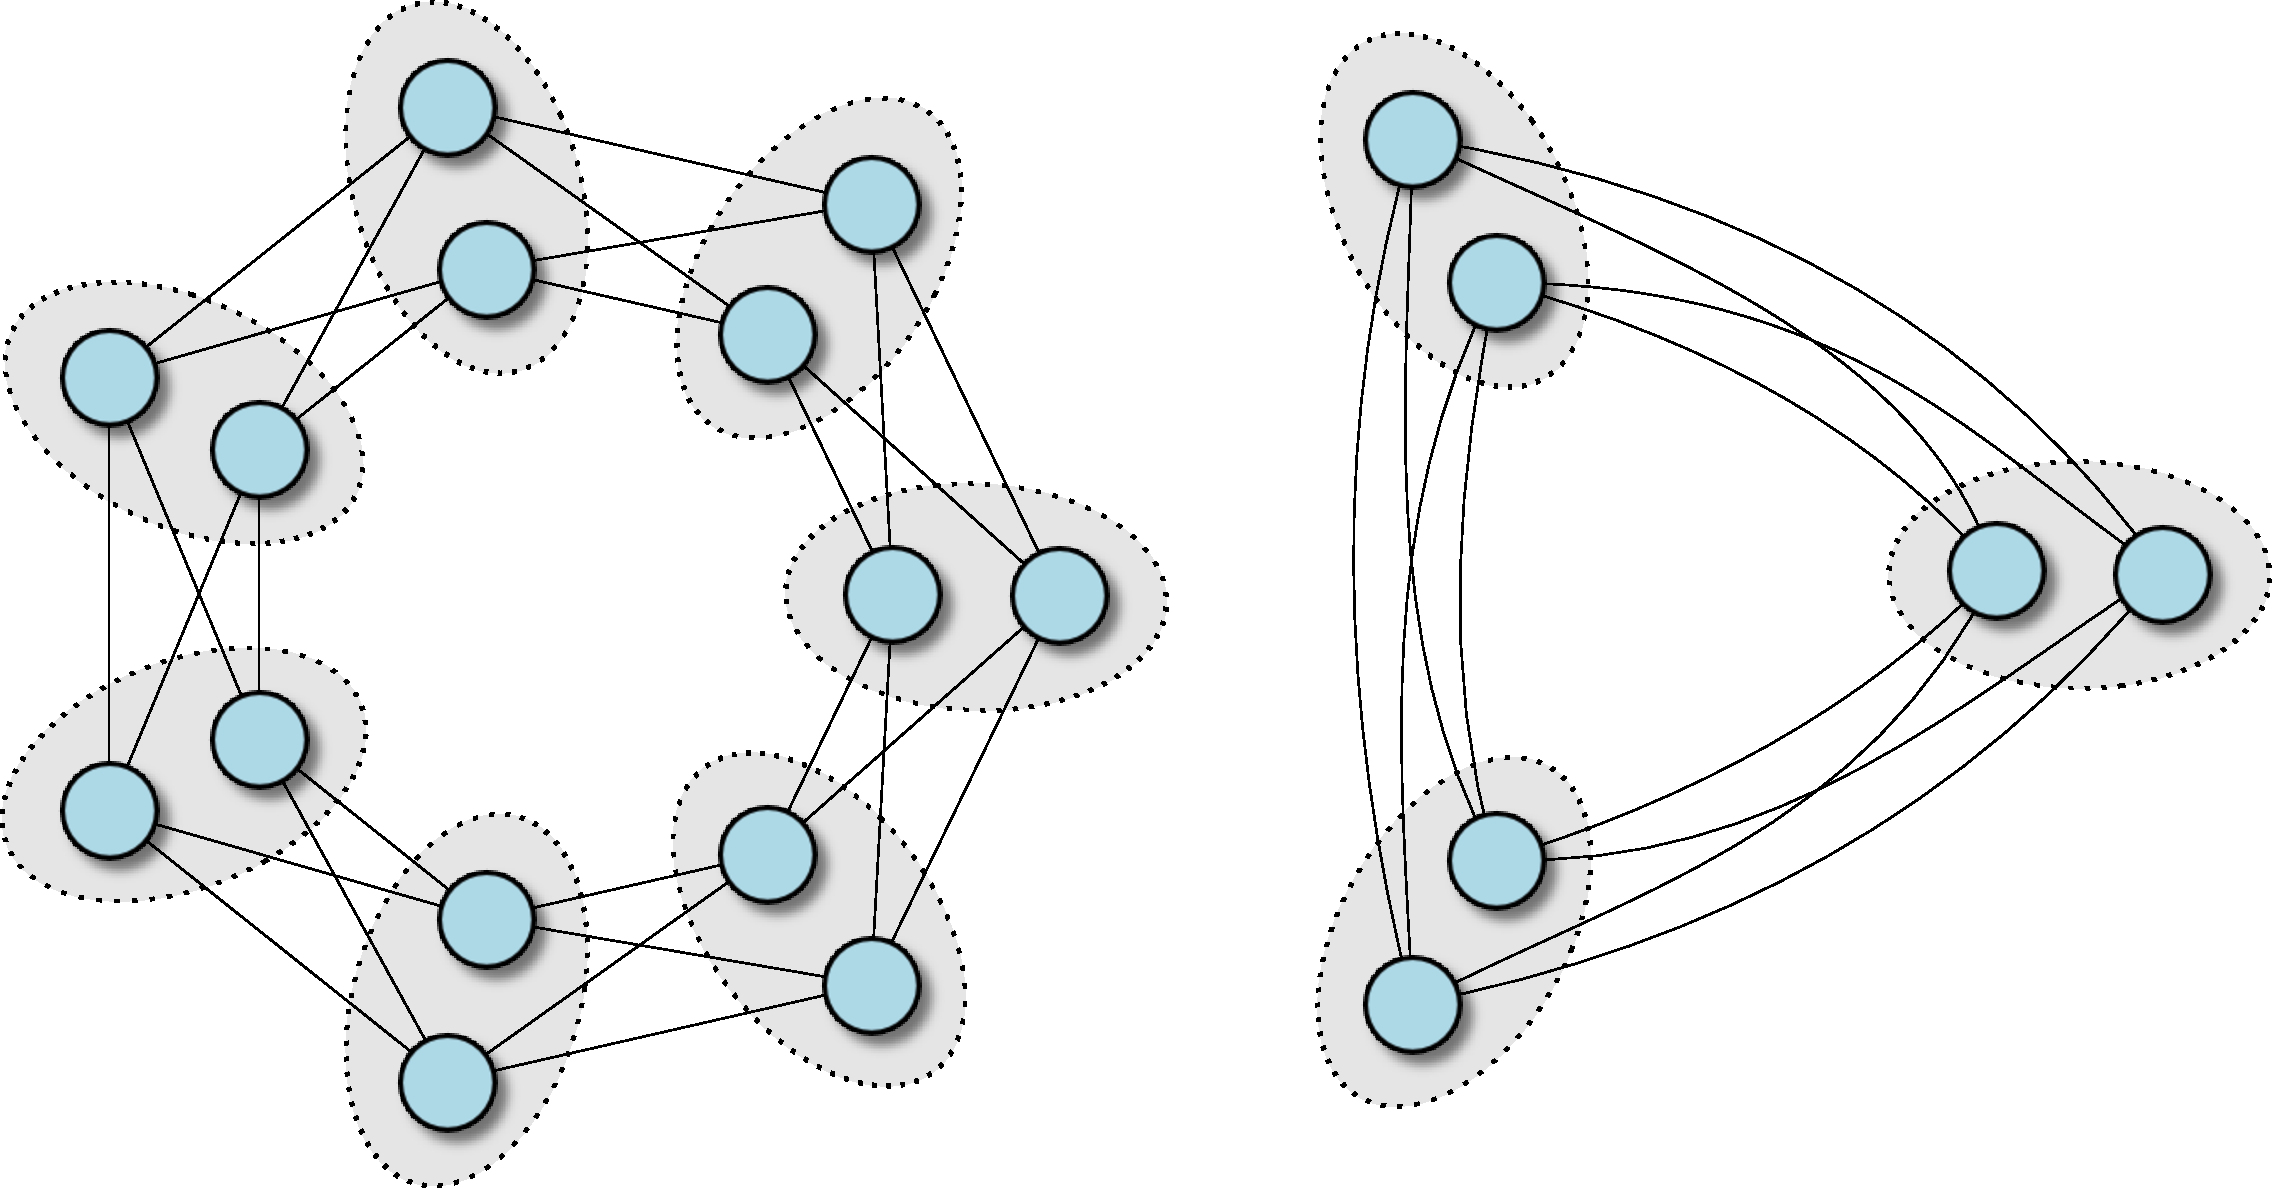
\includegraphics[width=.28\textwidth]{../pics/3-7-zigzag}}\hspace{2ex} \framebox{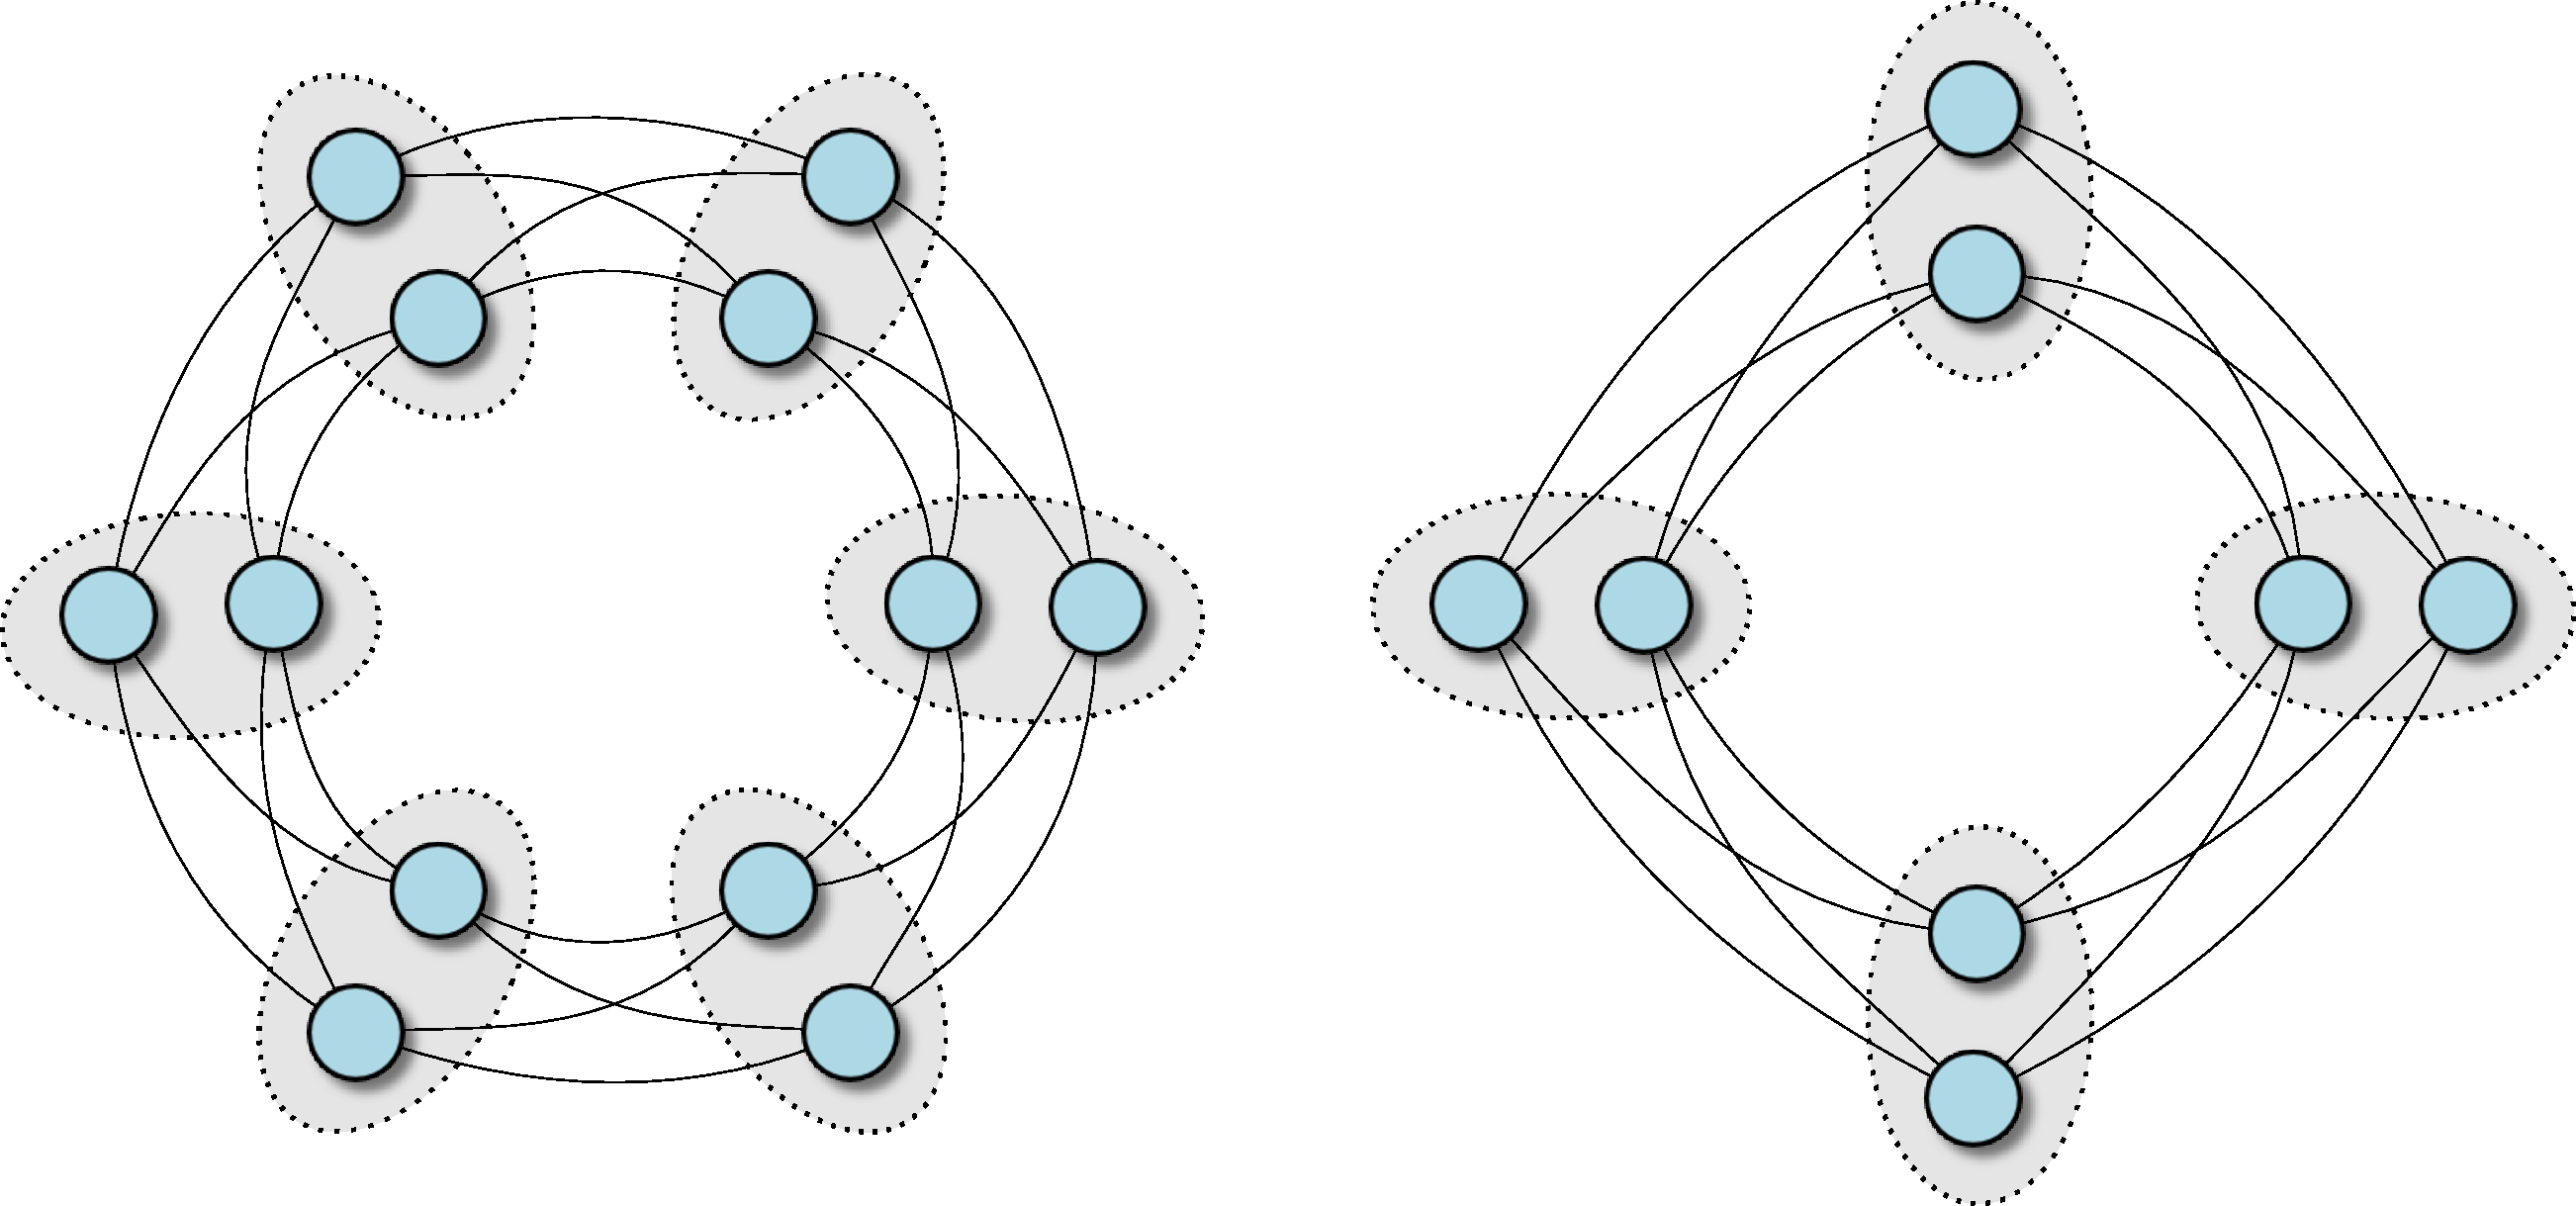
\includegraphics[width=.28\textwidth]{../pics/4-6-zigzag}} \hspace{2ex} \framebox{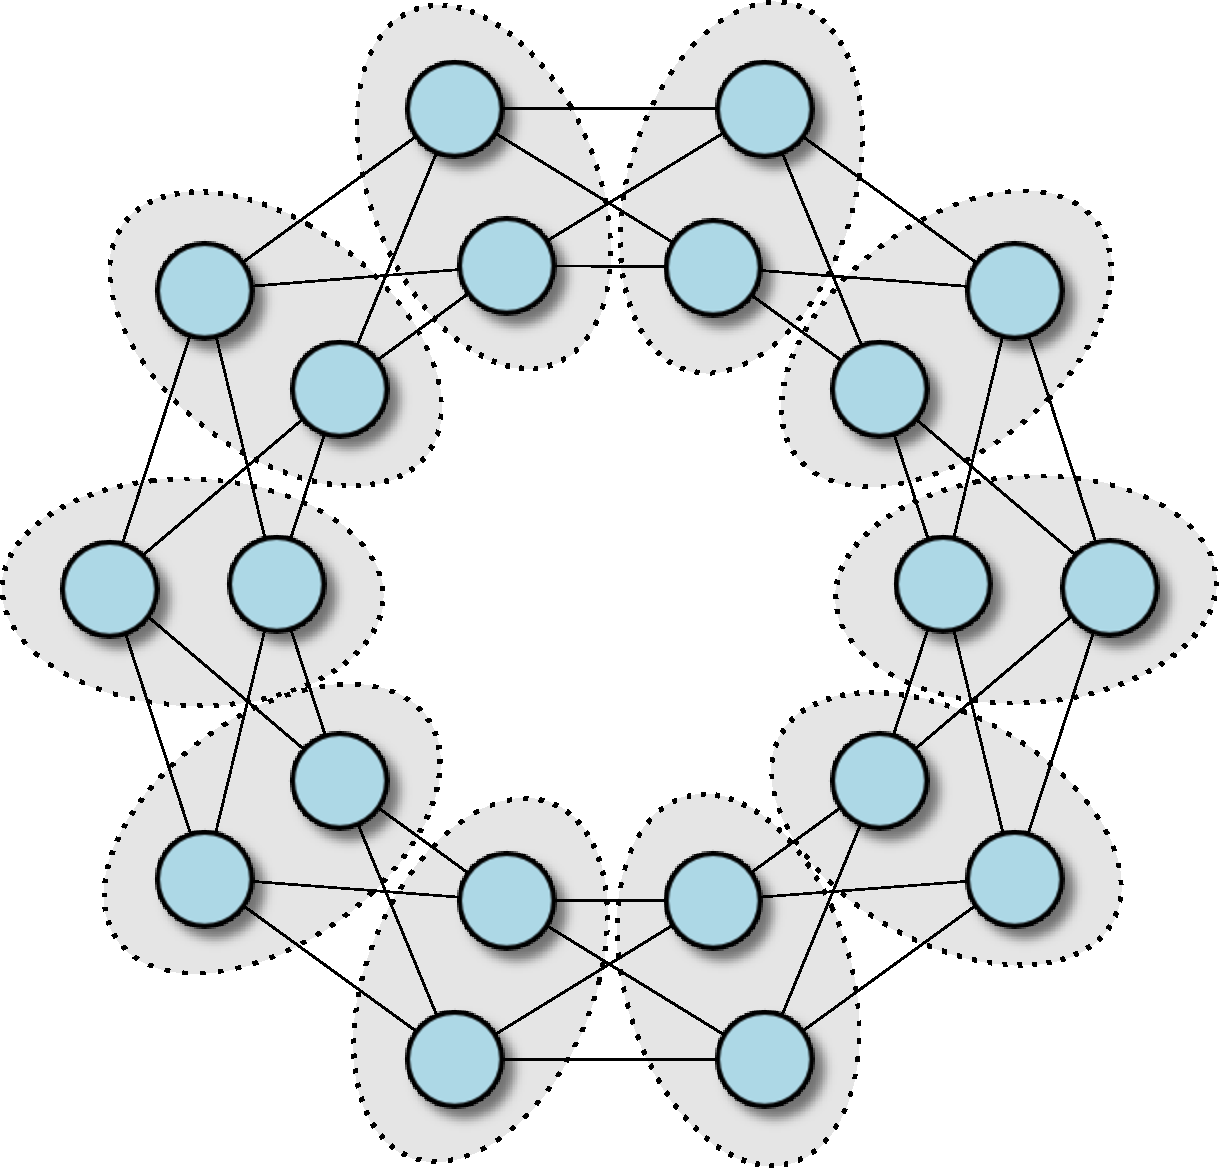
\includegraphics[width=.25\textwidth]{../pics/10-zigzag}}
    \end{center}
  \end{block}
\end{frame}

\begin{frame}{Purpose of Thesis (Expanded)}
  \begin{block}<1->{What is the goal?}
    \begin{itemize}
    \item To highlight how the \alert{enumeration} of $G$ with respect to $H$ effects the replacement and zig-zag products. 
    \end{itemize} 
  \end{block}
  \begin{block}<2->{How we will accomplish this?}
    \begin{enumerate}
      \item<3-> Define the zig-zag, and related, {\em replacement} products on regular graphs. (with small changes)
      \item<4->  Develop a complete characterization of the different classes of zig-zag and replacement products of a small, but non-trivial, special case.
      \item<5-> Present a generalization of the zig-zag product that will be called the {\em sandwich product}. (which will allow for many of the restrictions on the constituent graphs to be removed)
    \end{enumerate}
  \end{block}  
\end{frame}

\part{The Replacement and Zig-Zag Products}
\section{Enumerations}

\begin{frame}{The Replacement and Zig-Zag Products}
  \begin{columns}
    \column{.50\textwidth}
    \begin{figure}[h]
      \centering
      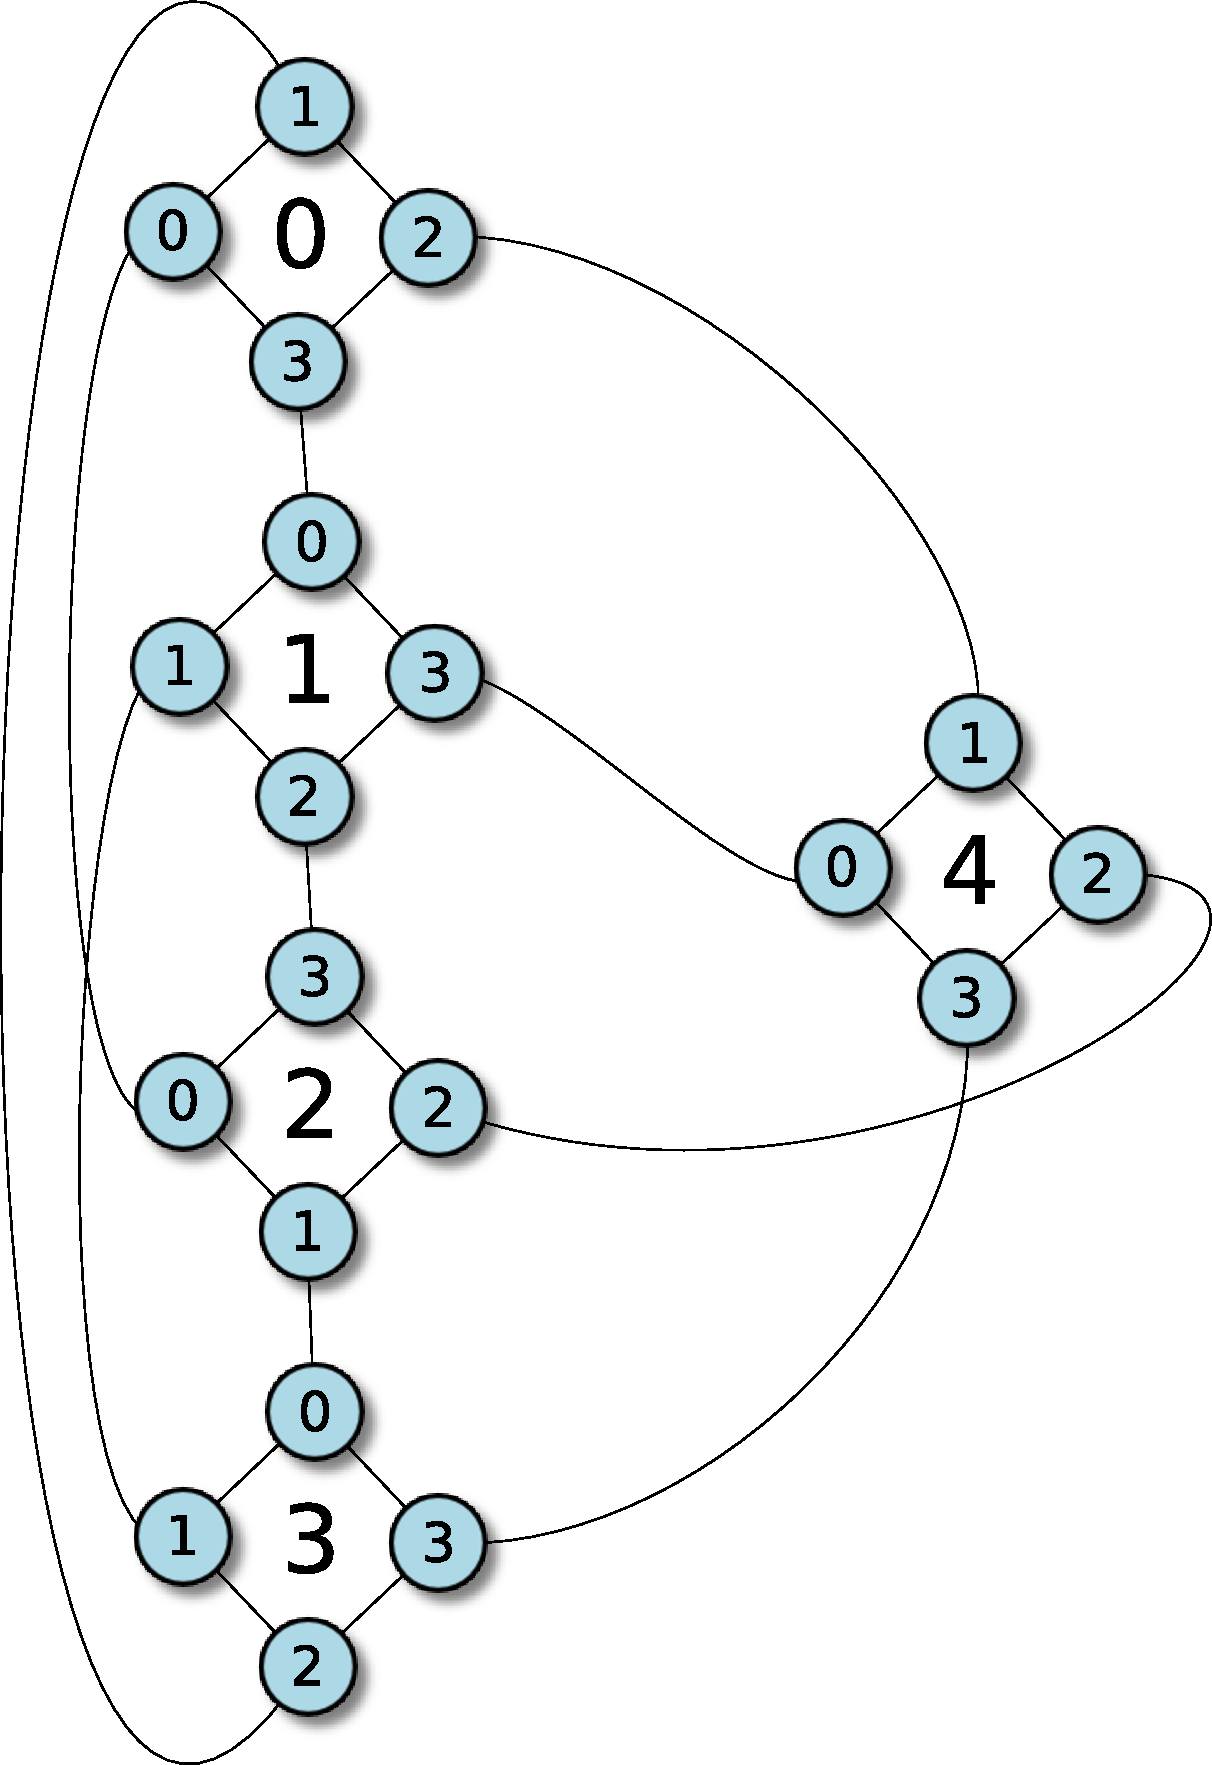
\includegraphics[width=.60\textwidth]{../pics/4-6-replacement-0123-043142}
      \caption{Example of $K_5 \protect\replacement C_4$}
      \label{fig:repl_ex}
    \end{figure}
    \column{.50\textwidth}
    \begin{figure}[h]
      \centering
      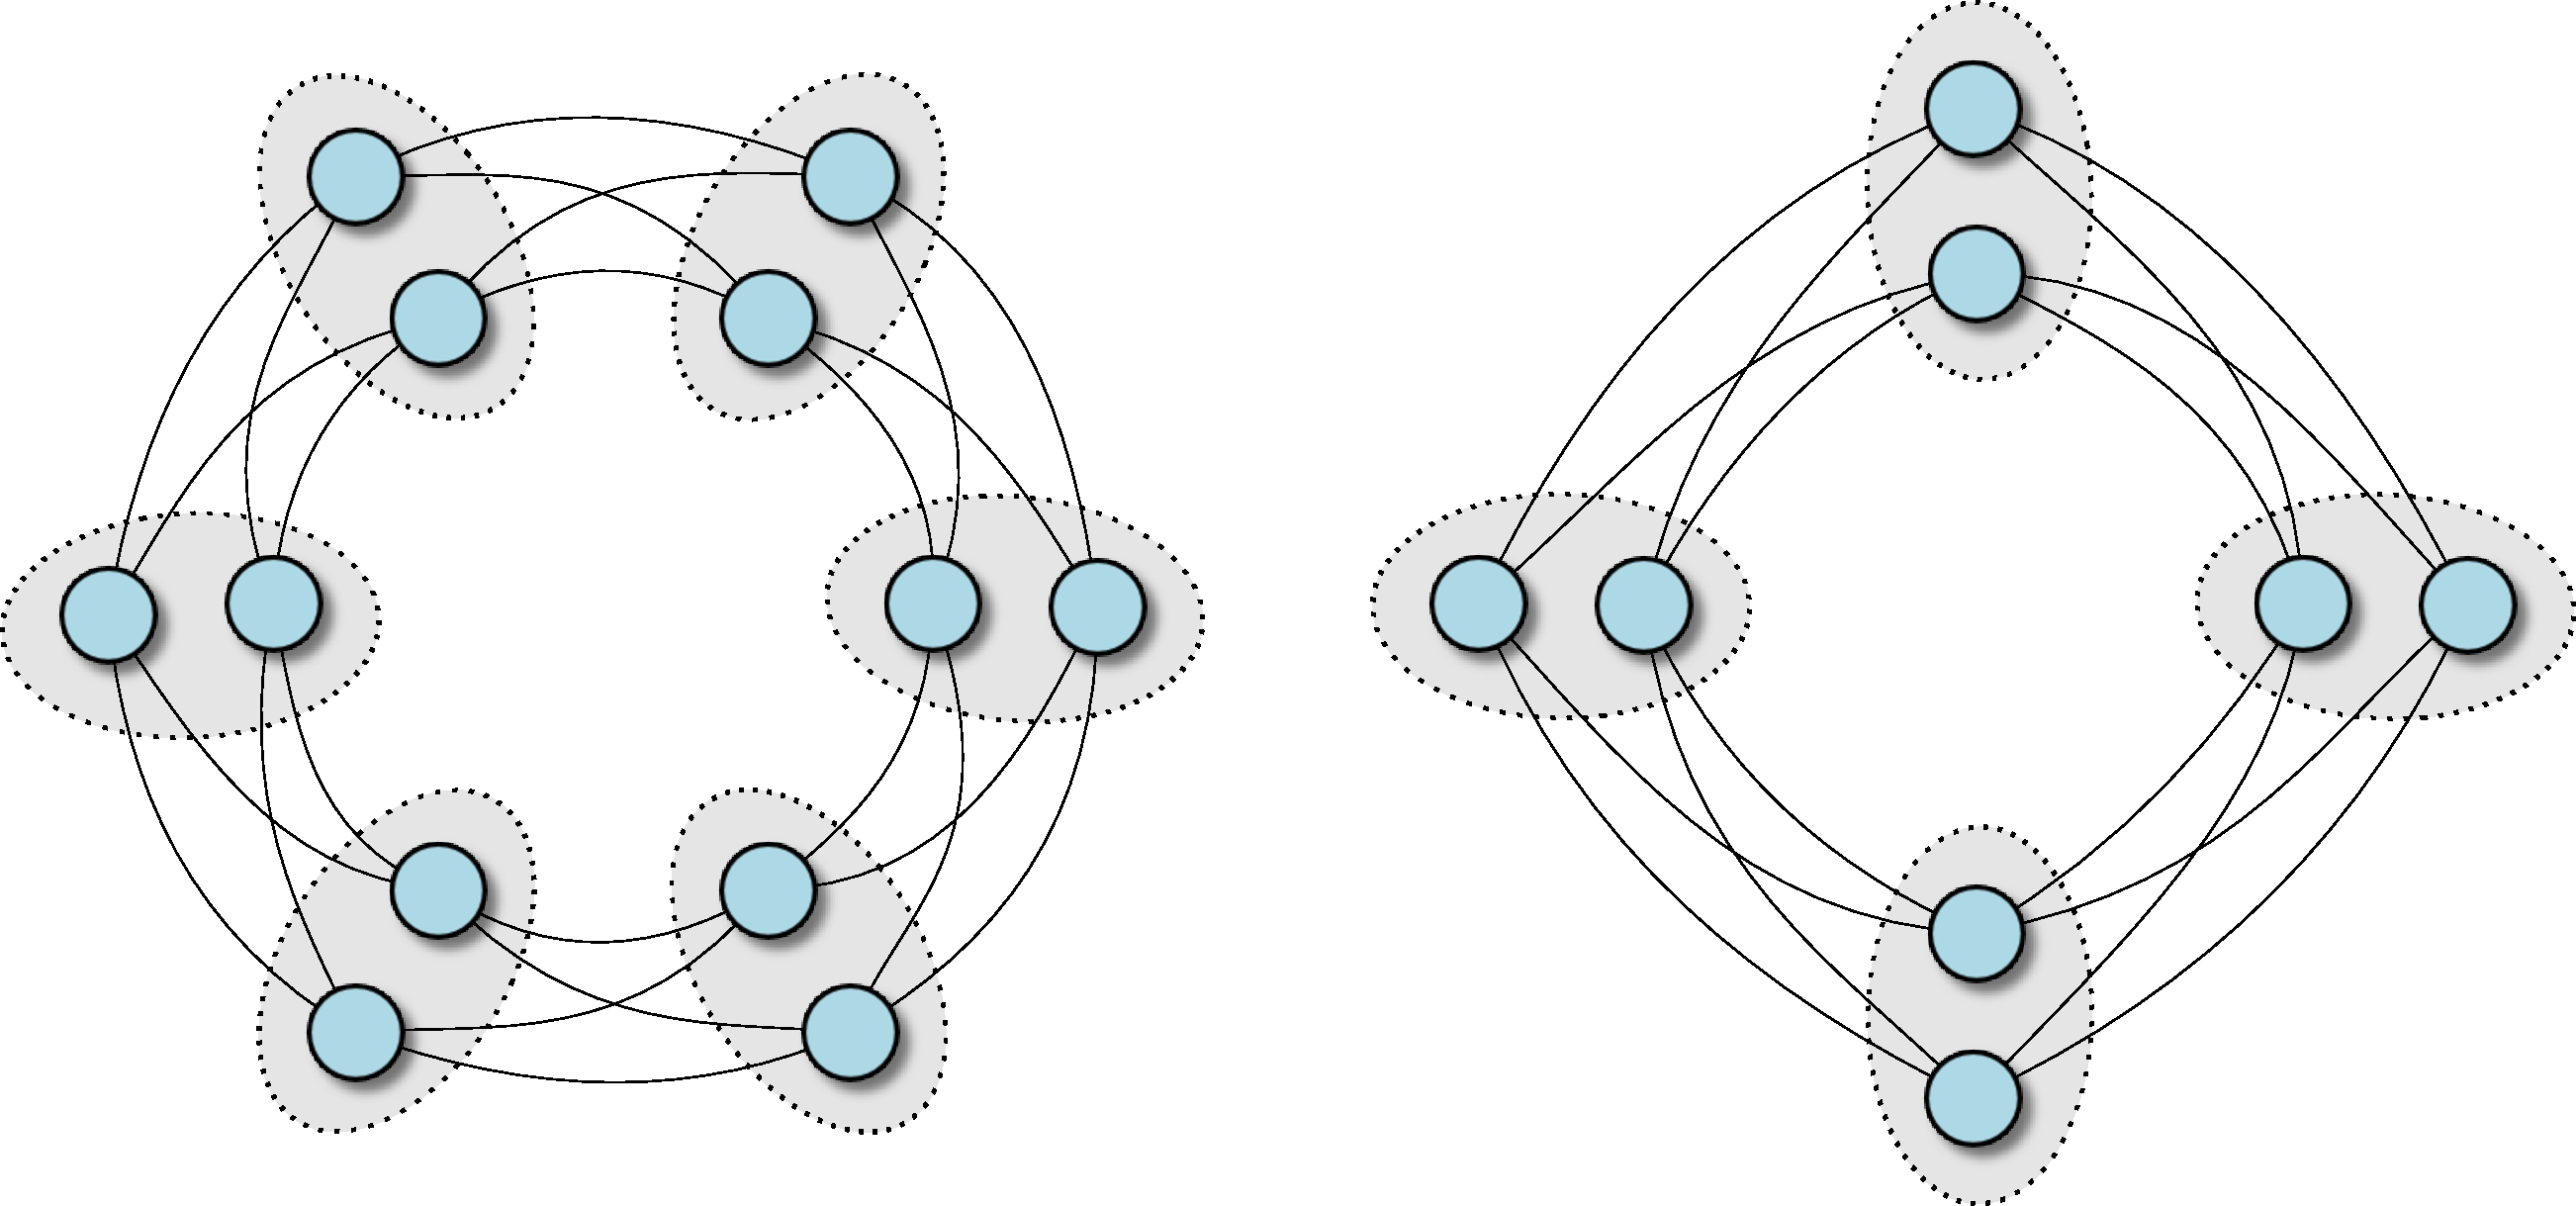
\includegraphics[width=.90\textwidth]{../pics/4-6-zigzag}
      \caption{Example of $K_5 \protect\zigzag C_4$}
      \label{fig:zz_ex}
    \end{figure}
  \end{columns}
  
\end{frame}

\begin{frame}{Definitions and Notation}
Let: 
\begin{itemize}
\item<2-> $G$ be a $m$-regular graph on $n$ vertices.
\item<3-> $H$ be a $d$-regular graph on $m$ vertices, $\left\{0,\ldots,m-1\right\}$.
\item<4-> $G$ and $H$ be both undirected and have no loops nor multi-edges.  
\item<5-> For each $u \in \vertS{G}$, $N_{u}$ be the set of vertices that are adjacent to $u$.

\item<6-> For each $u \in \vertS{G}$, define a bijection $\enum_{u}: N_{u} \to \vertS{H}$ which we will call the {\bf local-enumeration} of $u$ with respect to $H$
\end{itemize}
\end{frame}

\begin{frame}{The Enumeration of $G$ with respect to $H$}

\begin{block}{}
Each local enumeration provides a one-to-one correspondence between the {\em vertices} adjacent to a vertex and the vertices of the other graph.   
\end{block}

\begin{block}{}
\only<1>{
  \begin{figure}[h]
    \centering
    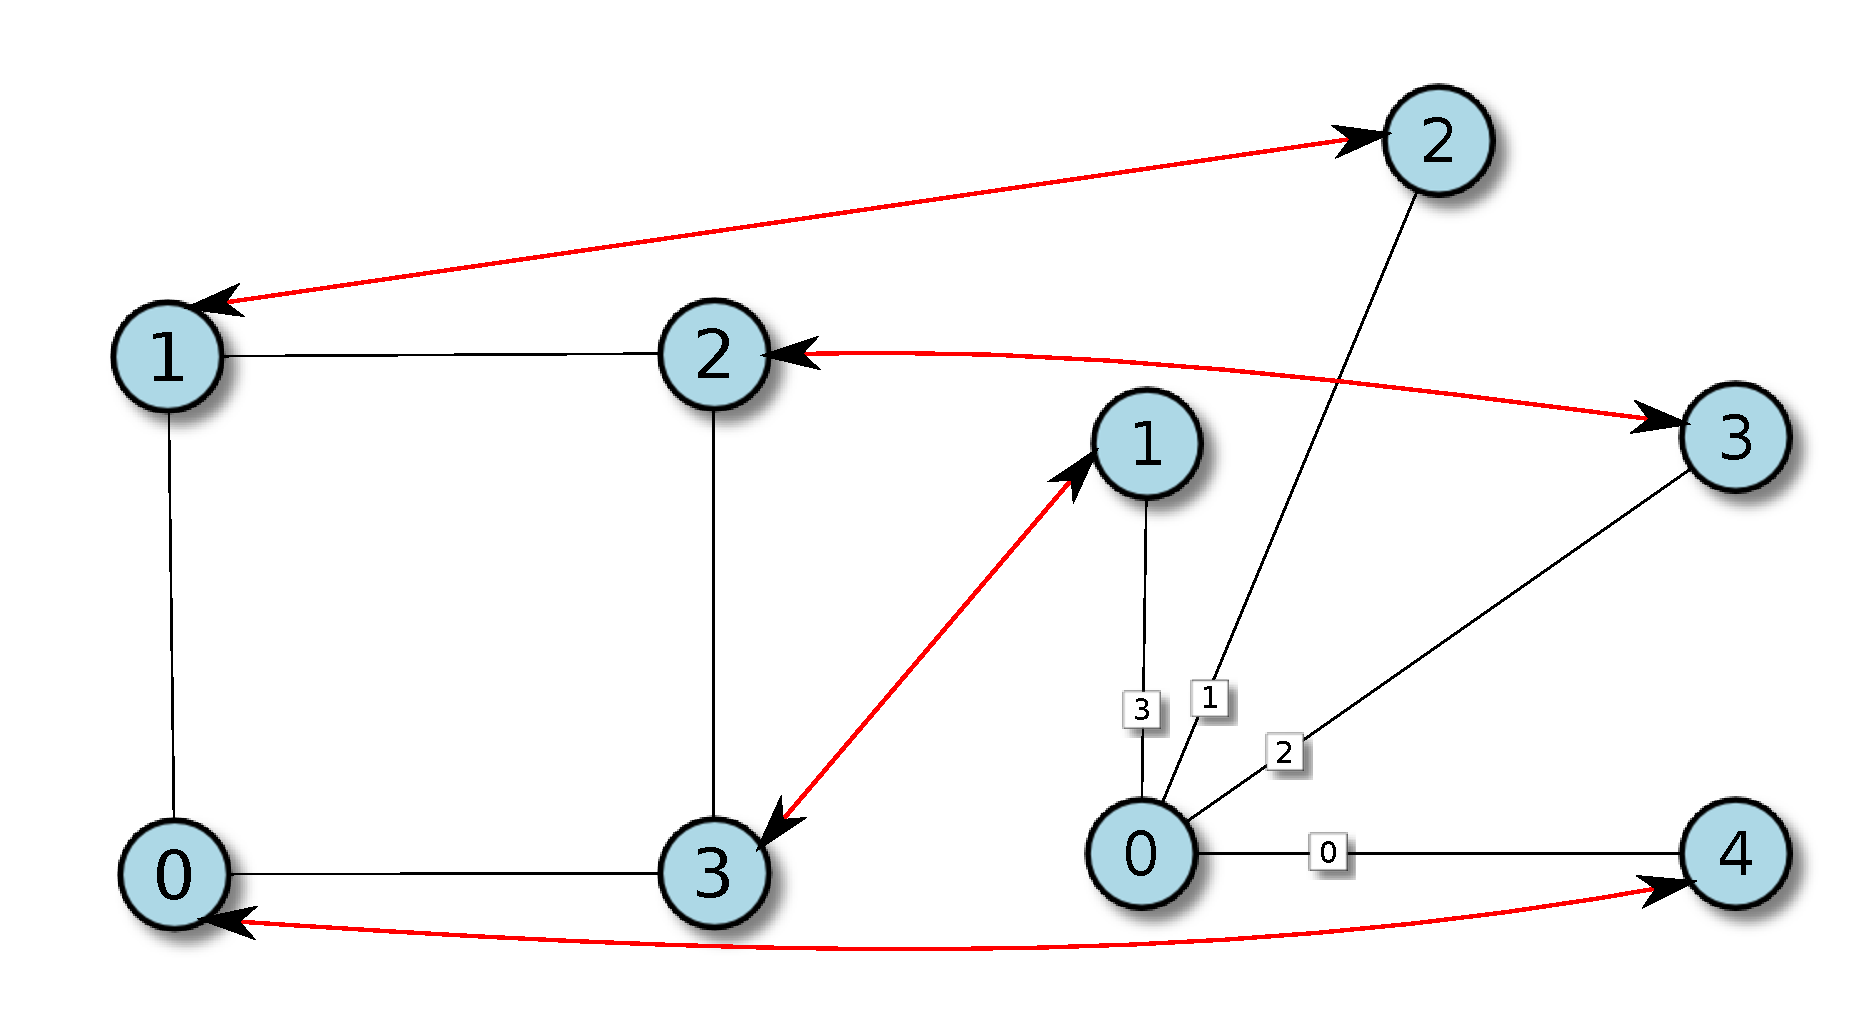
\includegraphics[height=.400\textheight]{../pics/0-enumeration}
    \caption{Example of a $0$-enumeration of $K_5$ with respect to $C_4$}
    \label{fig:0enum}
  \end{figure}
}
\only<2>{
  \begin{figure}[h]
    \centering
    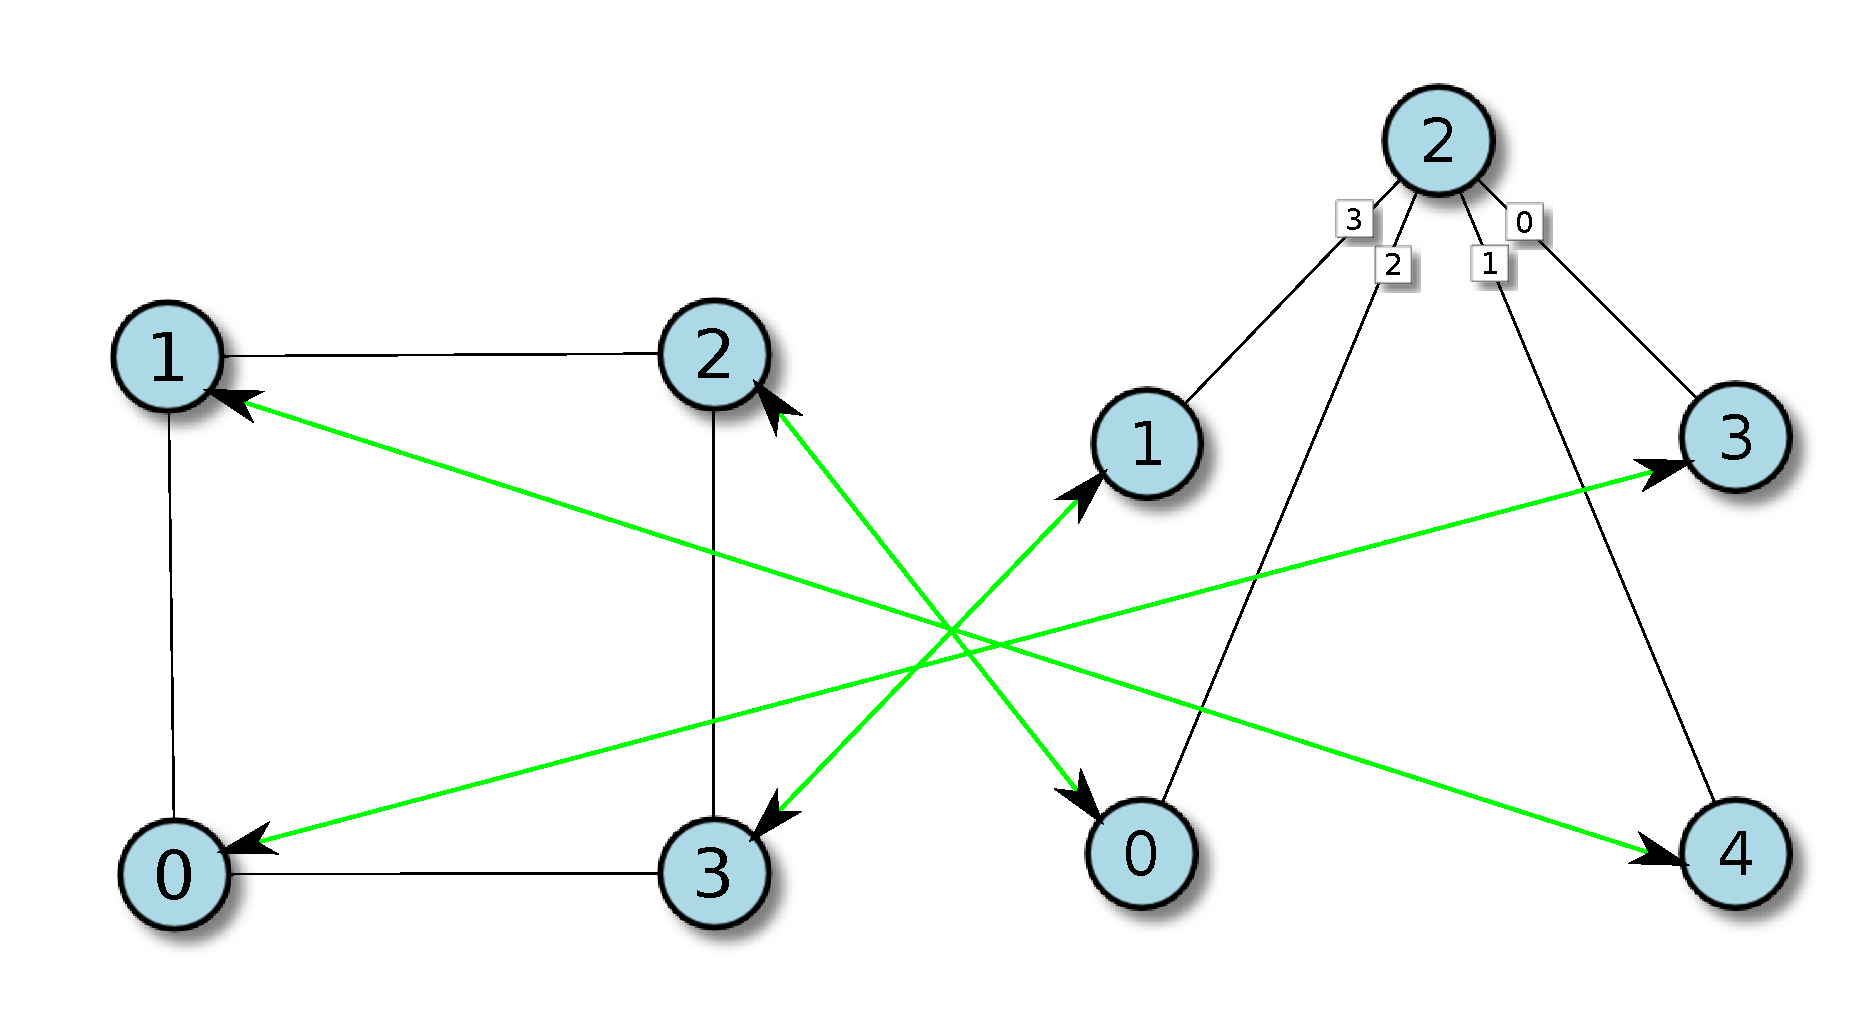
\includegraphics[height=.400\textheight]{../pics/2-enumeration}
    \caption{An example of a $2$-enumeration of $K_5$ with respect to $C_4$}
    \label{fig:2enum}
  \end{figure}
}

\only<3>{
  \begin{figure}[h]
    \centering
    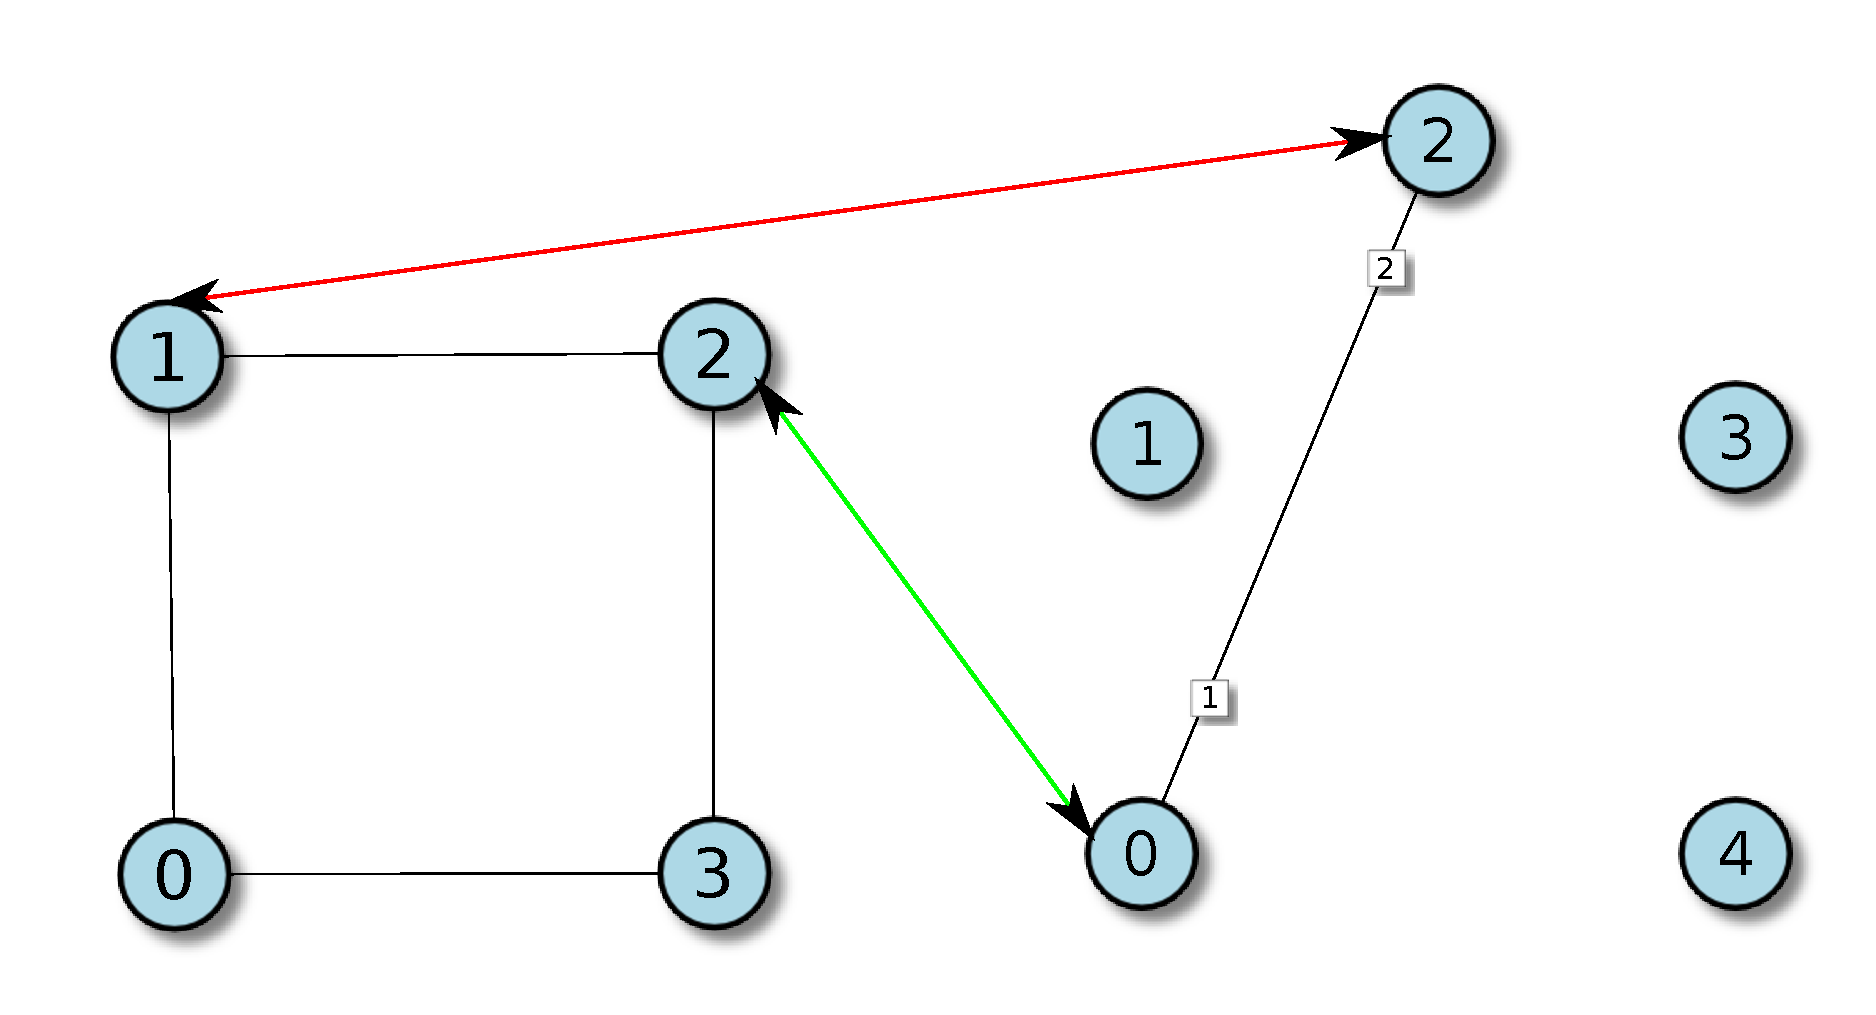
\includegraphics[height=.400\textheight]{../pics/(0,2)-enumeration}
    \caption{How two enumerations effect a single edge}
    \label{fig:02}
  \end{figure}
}
\end{block}
\end{frame}

\begin{frame}{Enumerations of $G$ with respect to $H$}
  \begin{block}{}
    We call the collection of local-enumerations of $G$ with respect to $H$  \[ \Enum = \left\{ \enum_{u}\ \vert\ u \in \vertS{G} \right\}      \] the {\em enumeration } of $G$. 
  \end{block}

  \begin{figure}[h]
    \centering
    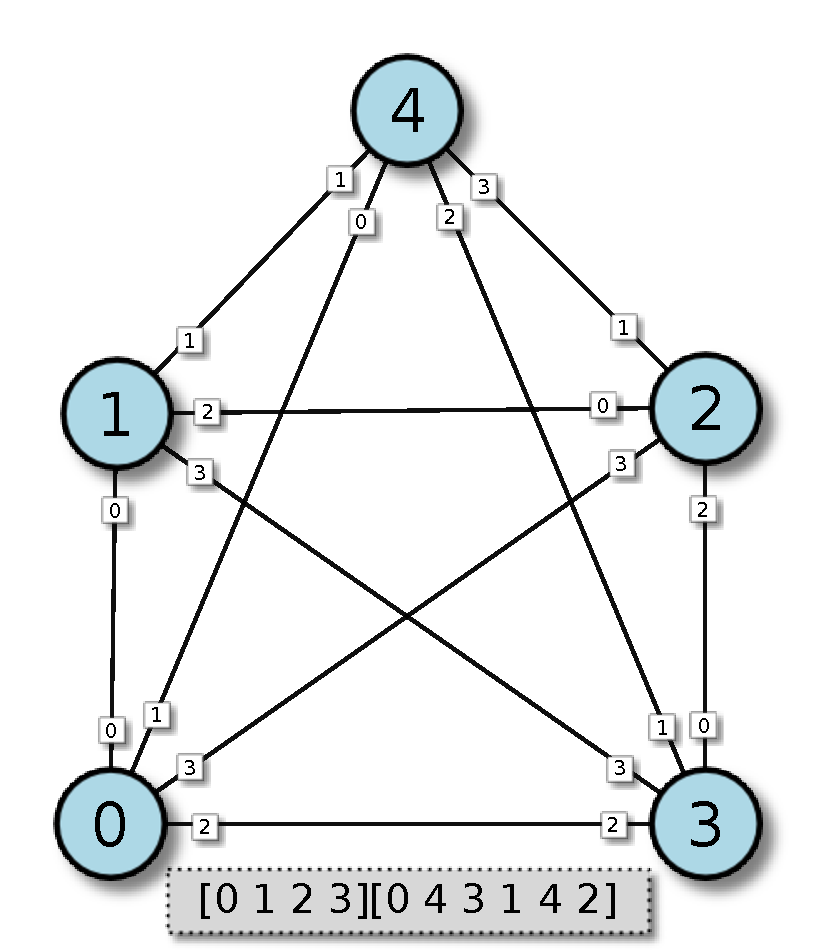
\includegraphics[height=.40\textheight]{../pics/K5-46-0123-043142}
    \caption{$K_5$ with an enumeration with respect to $C_4$ }
    \label{fig:k5enum}
  \end{figure}
  
\end{frame}

\section{The Replacement Product}
\begin{frame}{Definition: The Replacement Product}
  \begin{definition}
\label{def:replacement_product}
The {\bf replacement} product of $G$ with $H$ and enumeration $\Enum$, denoted $G \replacement_{\Enum} H$, is the graph with vertex set $\vertS{G} \times \vertS{H}$ for which $\left( u, a \right)$ is adjacent to $ \left( v, b \right)$ if either
\begin{enumerate}
\item \label{itm:rep_zig} $u = v$ and $\left( a, b\right) \in E(H)$, or
\item  \label{itm:rep_zag} $u \neq v$ and  $\left( u, v \right) \in \edgeS{G}$ where $\enum_{u}\left( v \right) = a $ and $\enum_{v}\left(u\right) = b$.
\end{enumerate}
\end{definition}

\begin{figure}[h]
  \centering
  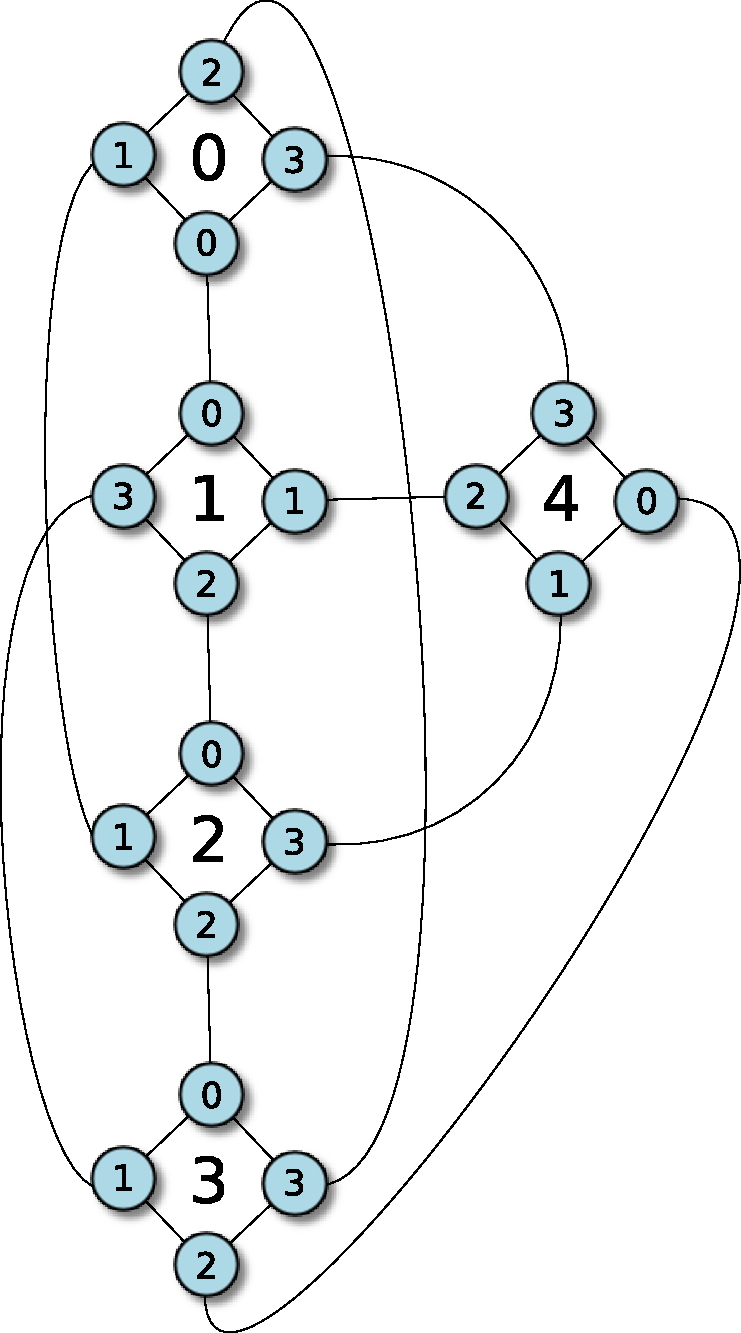
\includegraphics[height=.35\textheight]{../pics/3-7-replacement-024-0123413}
  \caption{Example of $K_5 \protect\replacement C_4$}
  \label{fig:repl_ex2}
\end{figure}
\end{frame}

\begin{frame}{The Replacement Product: Clouds and Bridges}
  \only<1>{The {\bf replacement product} is the disjoint union of two graphs.}
  \begin{columns}
    \column{.50\textwidth}
    \begin{enumerate}
      \item<2-> $u = v$ and $\left( a, b\right) \in E(H)$ (Clouds)
      \item<3-> $u \neq v$ and  $\left( u, v \right) \in \edgeS{G}$ where $\enum_{u}\left( v \right) = a $ and $\enum_{v}\left(u\right) = b$. (Bridges)
    \end{enumerate}
    \column{.50\textwidth}
    \only<2>{
      \begin{figure}[h]
        \centering
        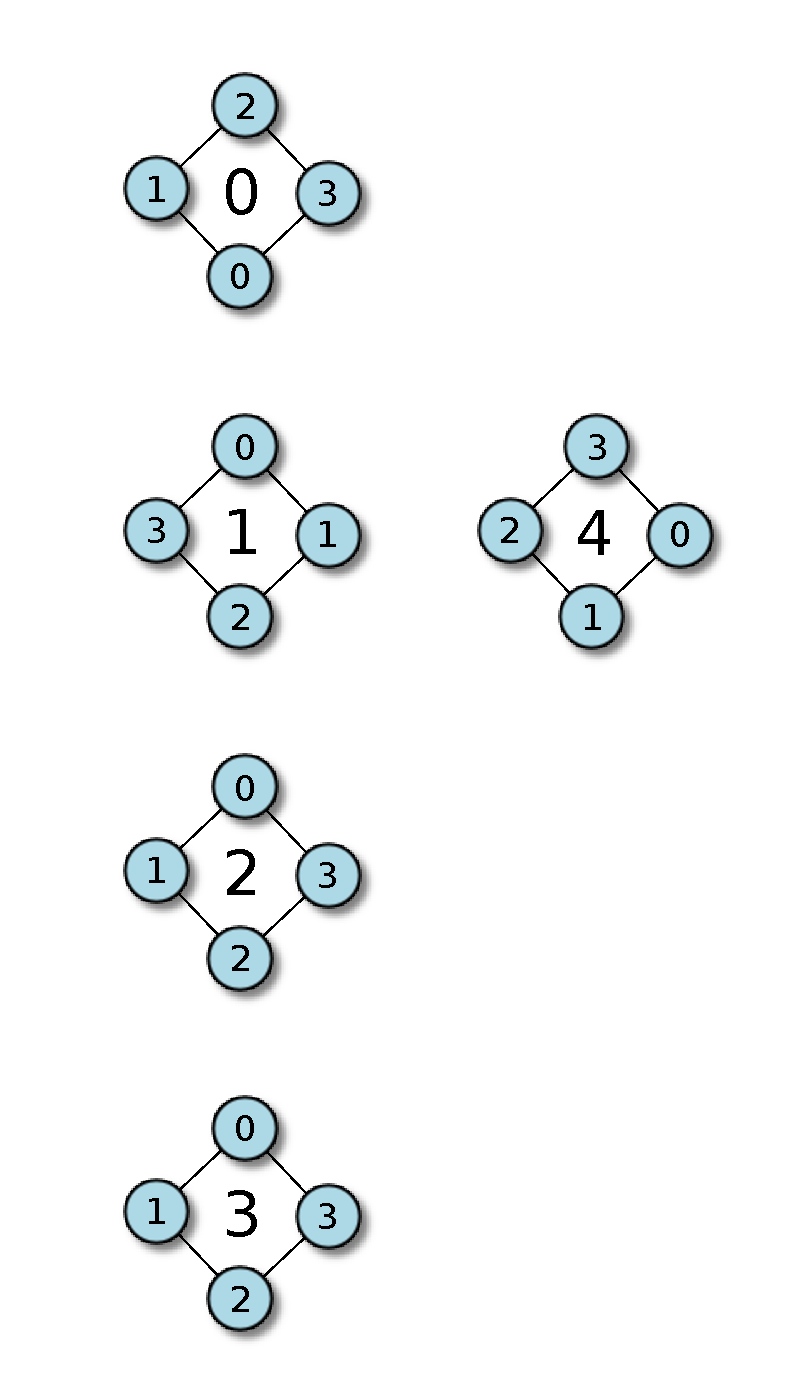
\includegraphics[width=.65\textwidth]{../pics/replacement-clouds}
        \caption{{\em clouds} in $K_5 \replacement C_4$ }
        \label{fig:replacement_clouds}
      \end{figure}}
    \only<3>{
      \begin{figure}[h]
        \centering
        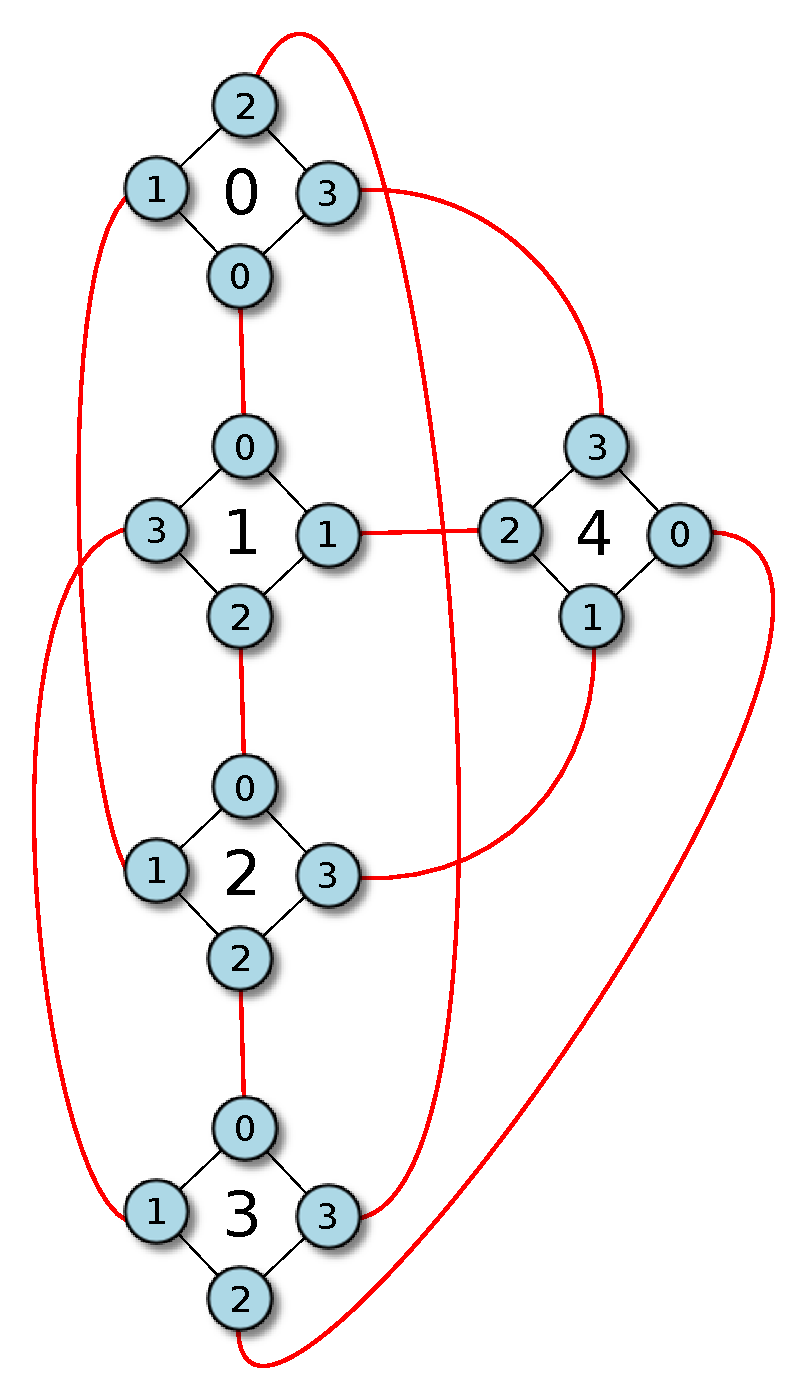
\includegraphics[width=.65\textwidth]{../pics/replacement-bridges}
        \caption{{\em bridges} in $K_5 \replacement C_4$ }
        \label{fig:replacement_clouds}
      \end{figure}
    }
  \end{columns}
\end{frame}
\begin{frame}{The Replacement Product: Different Enumerations}
  \begin{columns}
    \column{.50\textwidth}
    \begin{itemize}
      \item<1-> The {\em clouds} are fixed, independent of enumeration.
      \item<2-> The {\em bridges} vary by enumeration.
    \end{itemize}
    \column{.50\textwidth}
    \only<1-2>{
      \begin{figure}[h]
        \centering
        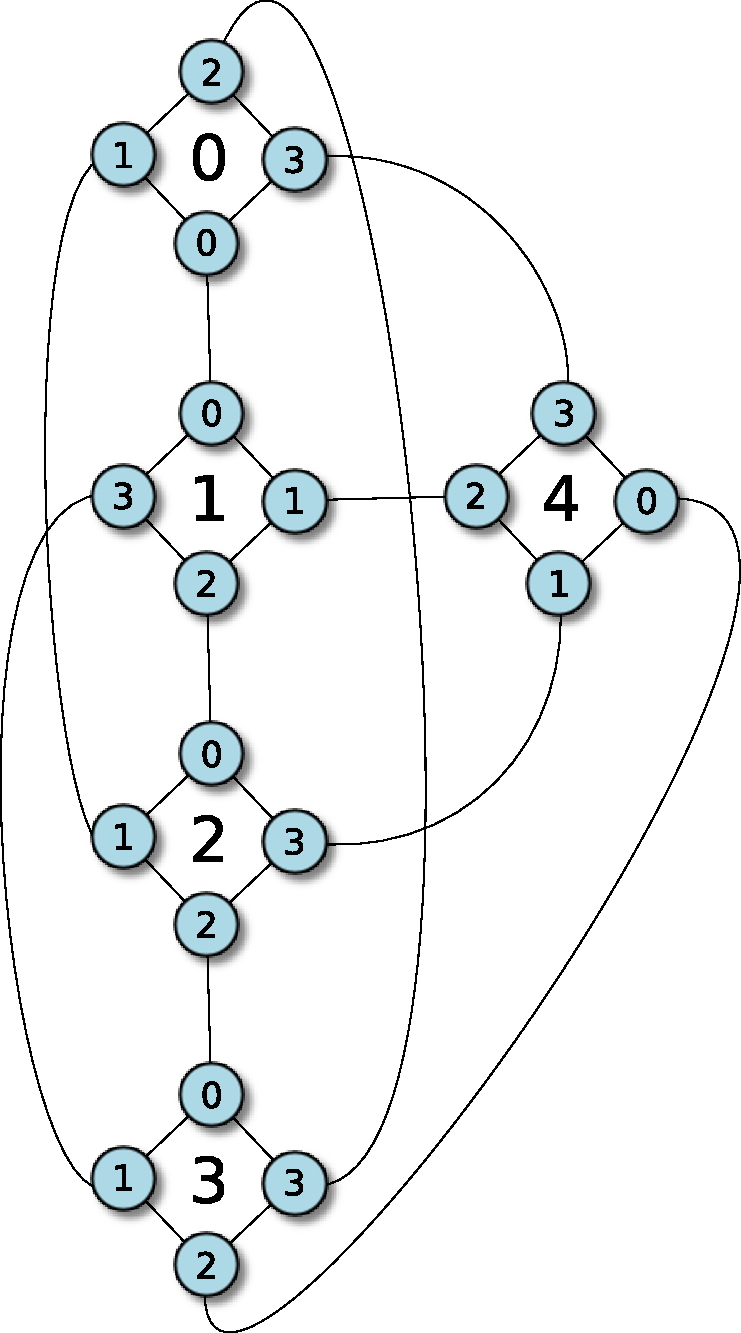
\includegraphics[width=.59\textwidth]{../pics/3-7-replacement-024-0123413}
        \caption{$K_5 \replacement C_4$ with a $3,7$ enumeration }
        \label{fig:replacement_clouds}
      \end{figure}}
    \only<3>{
      \begin{figure}[h]
        \centering
        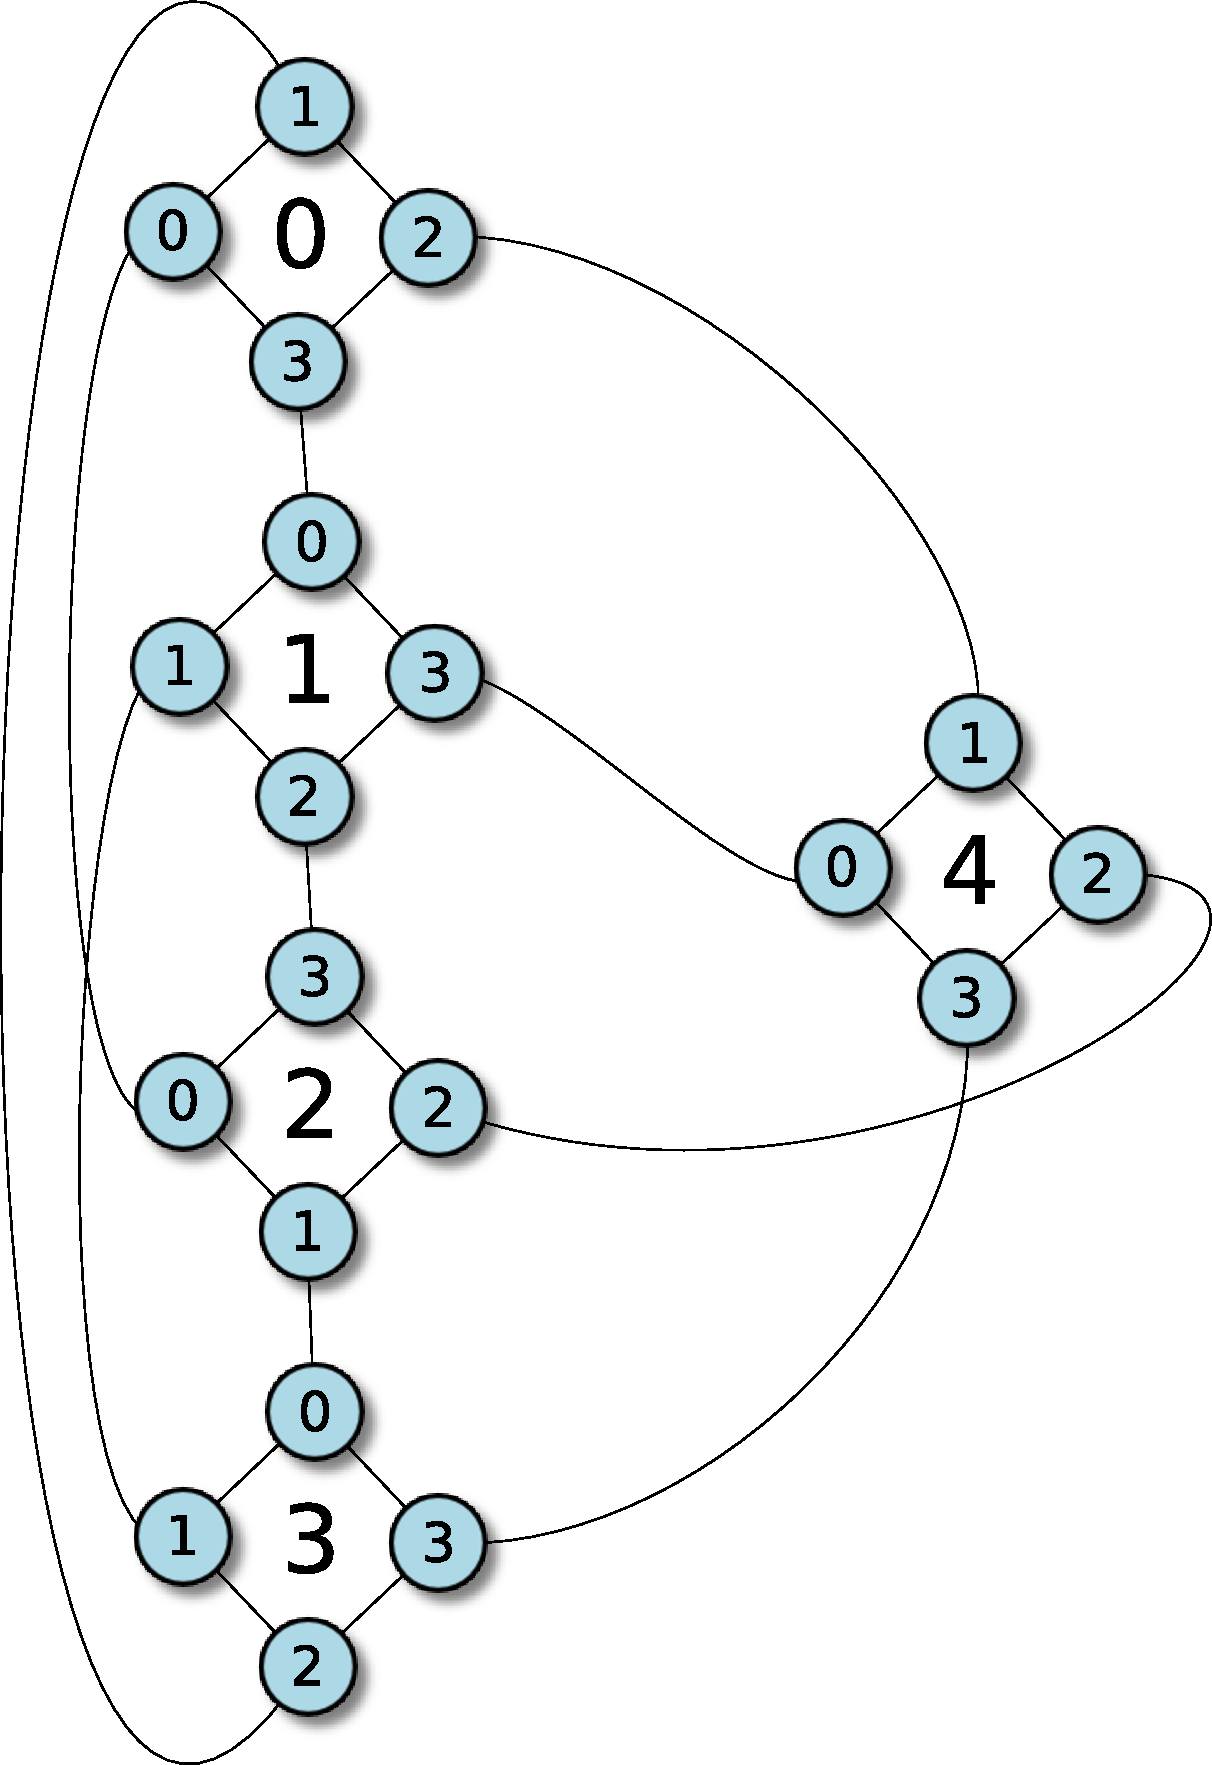
\includegraphics[width=.61\textwidth]{../pics/4-6-replacement-0123-043142}
        \caption{$K_5 \replacement C_4$ with a $4,6$ enumeration}
        \label{fig:replacement_clouds}
      \end{figure}
    }
  \end{columns}
\end{frame}
\begin{frame}{Bridges and Enumerations}
  \begin{columns}
    \column{.50\textwidth}
    \begin{block}{}
      Each bridge edge is of the form \[ \left(\left(u, \enum_u(v) \right),\left(v, \enum_v(u)\right)\right)\]
    \end{block}
    \column{.50\textwidth}
    \begin{figure}[h]
      \centering
        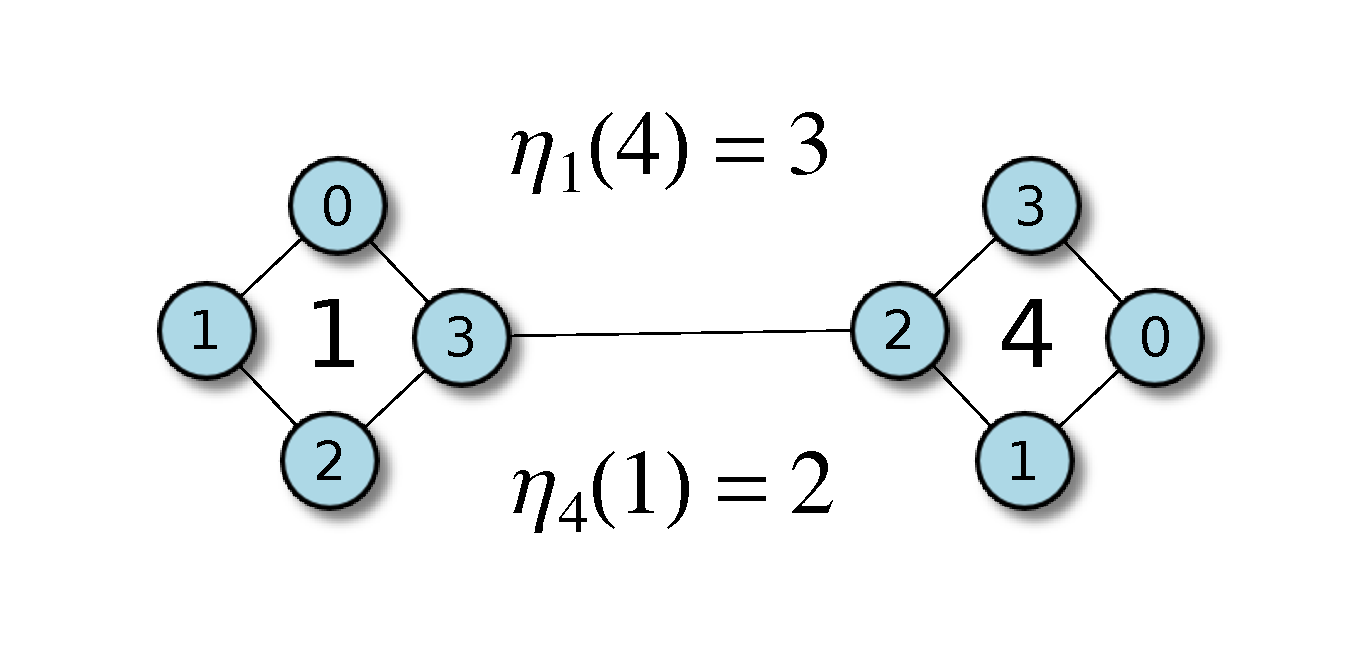
\includegraphics[width=\textwidth]{../pics/bridge}
      \caption{A {\em bridge} and the local-enumeration.}
      \label{fig:bridge}
    \end{figure}
  \end{columns}
\end{frame}
\begin{frame}{Non Isomorphic Replacement Products}
  \begin{columns}
    \column{.50\textwidth}
    \begin{figure}[h]
      \centering
         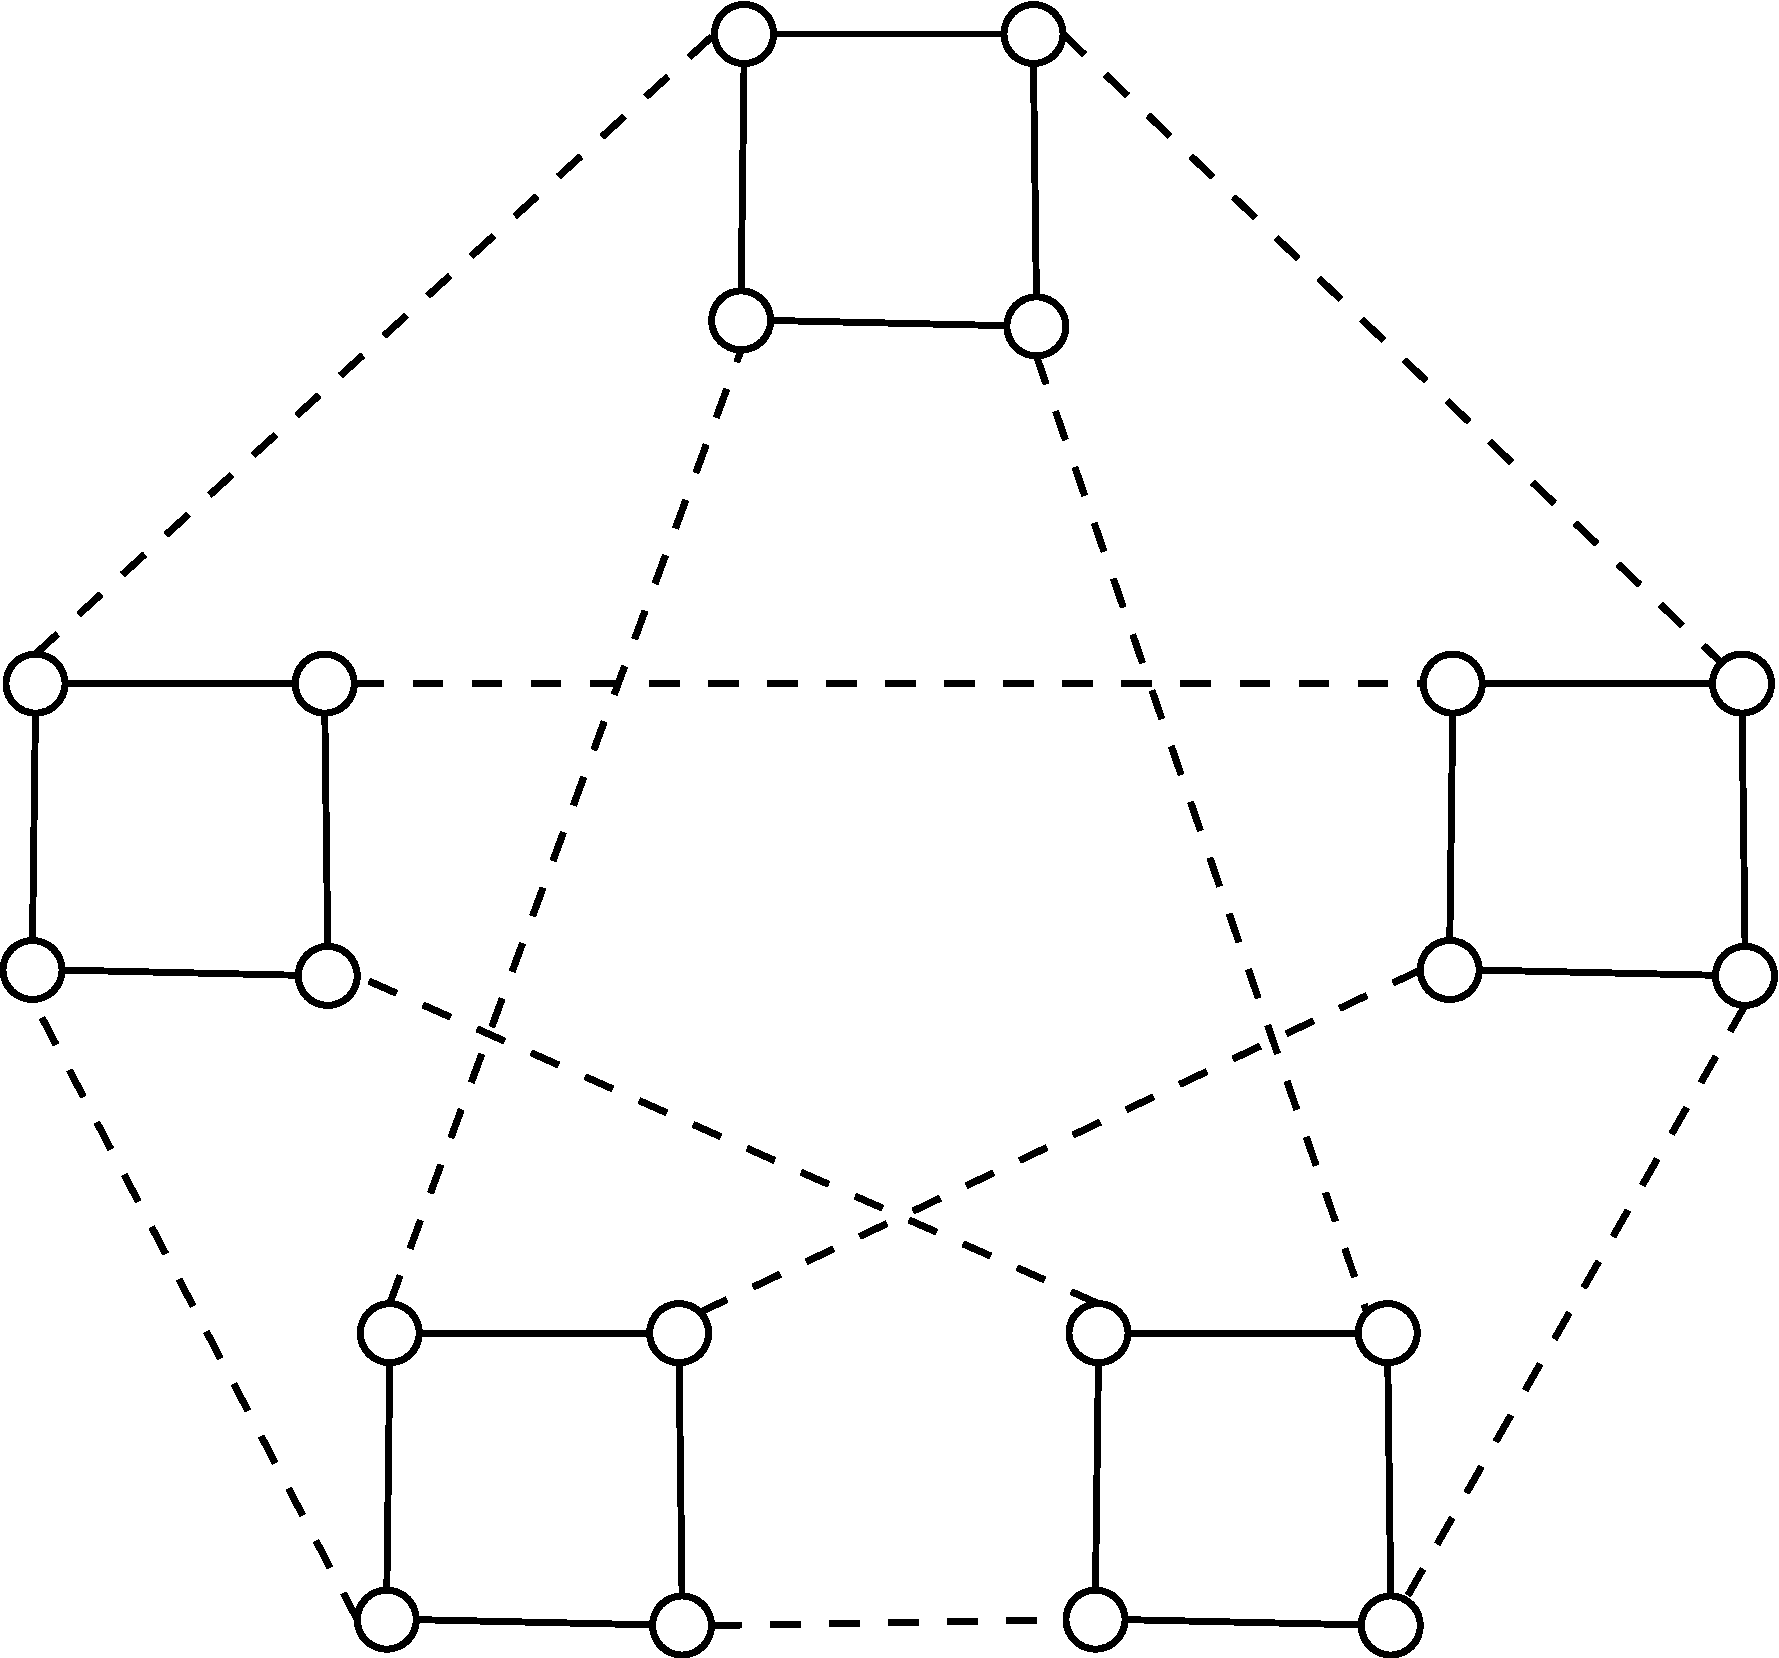
\includegraphics[width=.7\textwidth]{../pics/replacementK5_C4}
      \caption{An example $K_5 \replacement C_4$ which is bipartite.}
    \end{figure}
    \column{.50\textwidth}
    \begin{figure}[h]
      \centering
        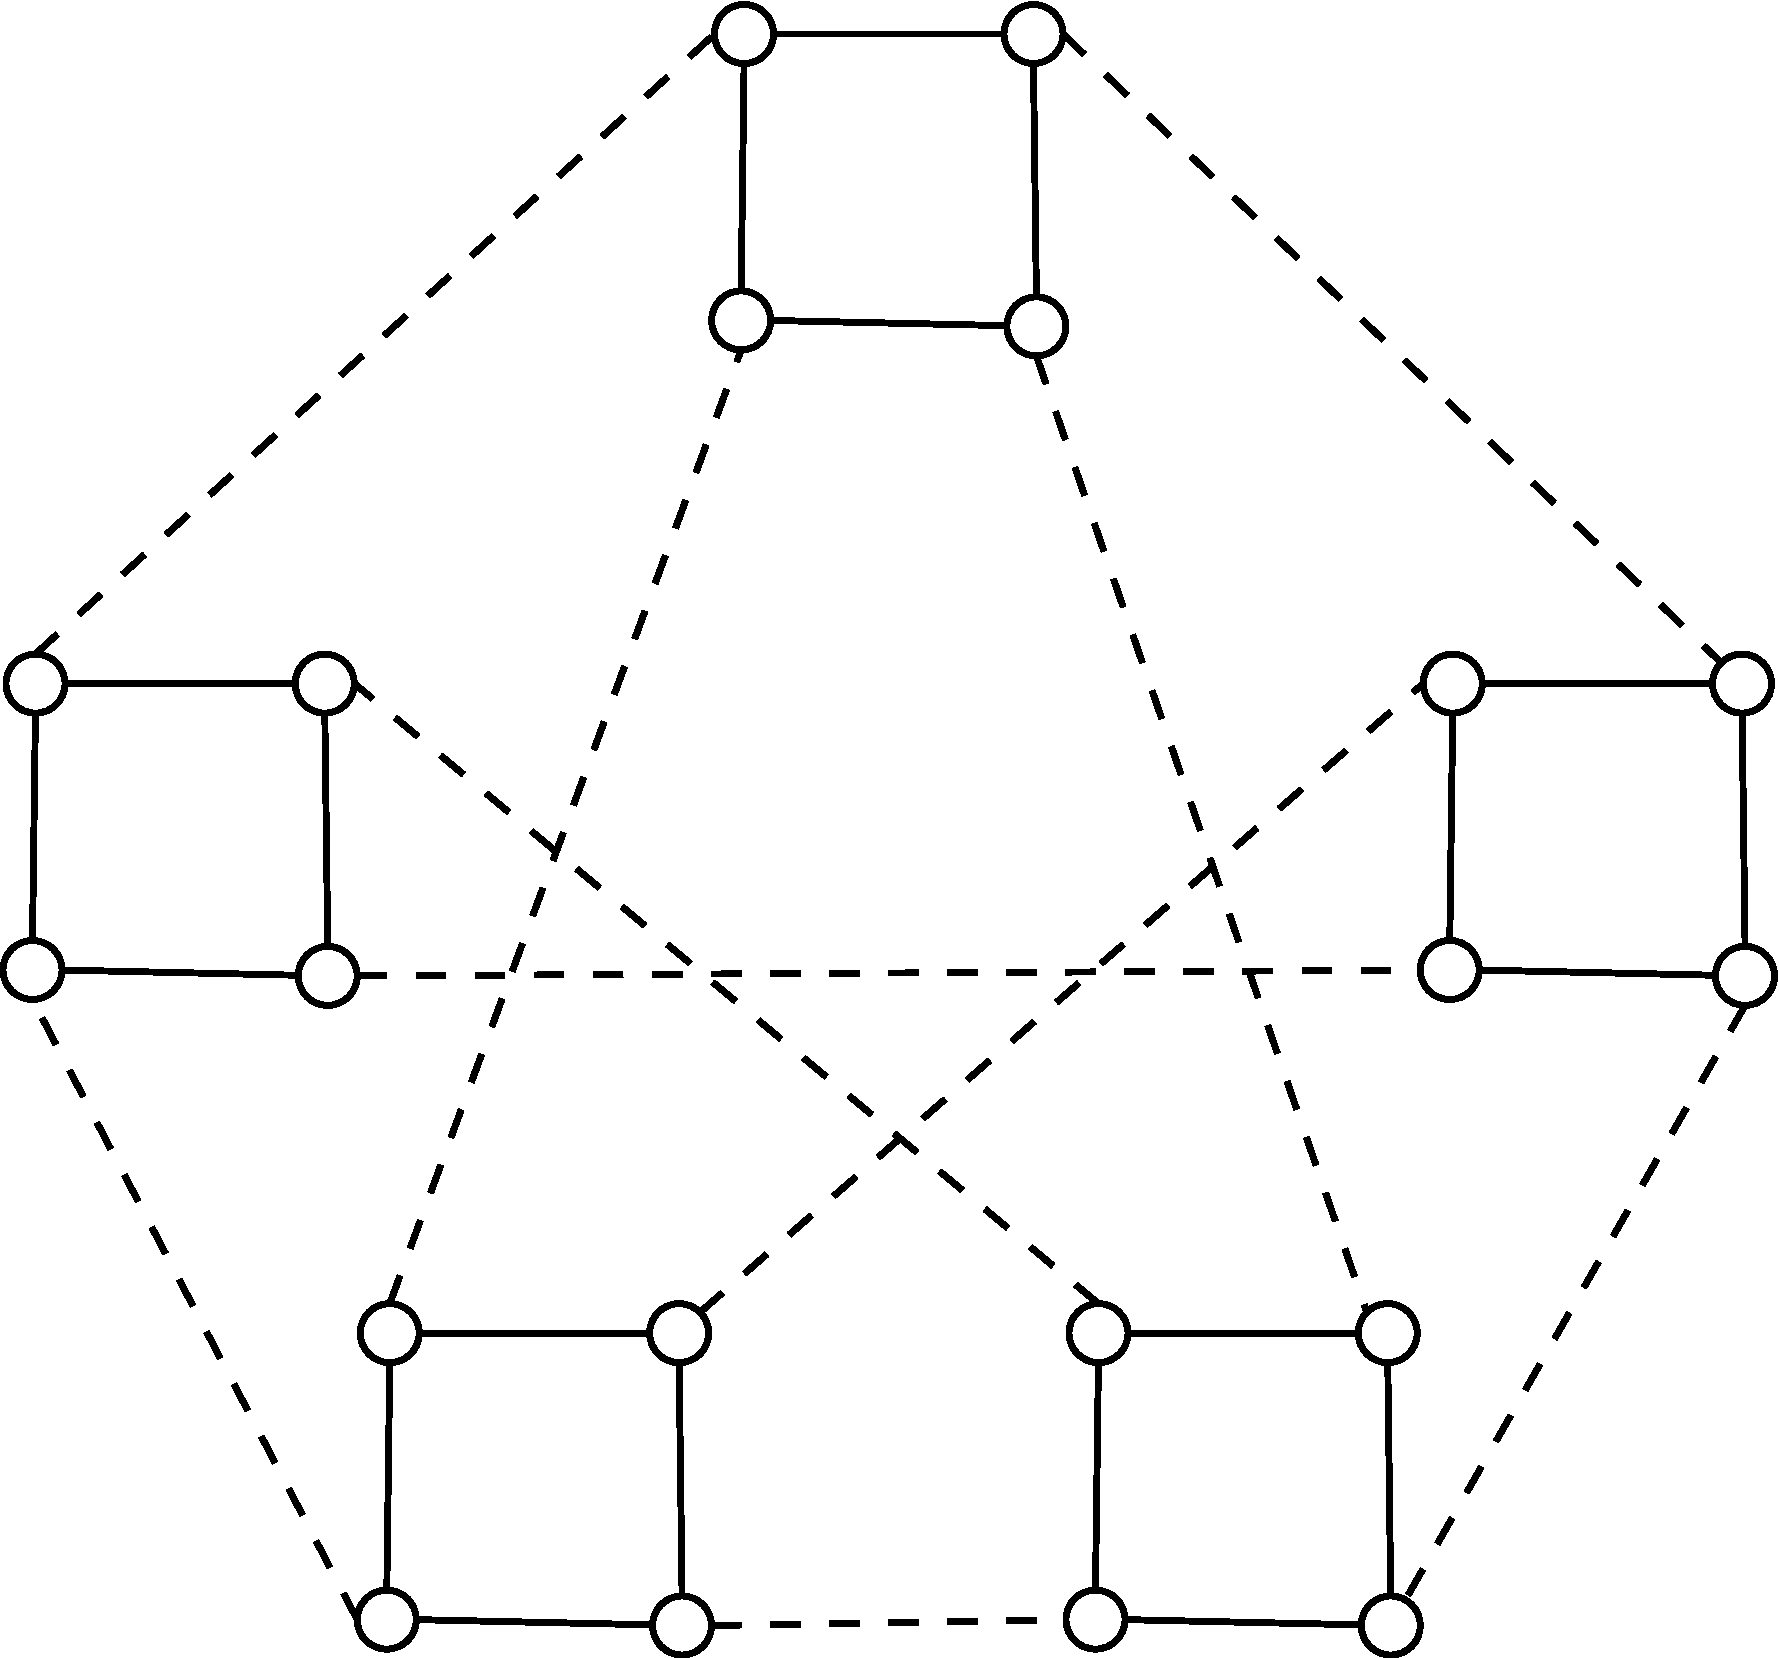
\includegraphics[width=.7\textwidth]{../pics/replacementK5_C4_2}
        \caption{Example $K_5 \protect\replacement C_4$ with odd cycles.}
        \label{fig:cycles_rep}
    \end{figure}
  \end{columns}
\end{frame}


\begin{frame}{The Replacement Product Isomorphism}
  \begin{definition}
\label{prop:replacement_prod_iso}
Let $\Enum$ and $\Enum^{\prime}$ be two enumerations and let $G \replacement H$ and $G \replacement^{\prime} H$ be the associated replacement products.  
  \begin{itemize}
    \item Let $f \in \Aut(G)$ and, for each $u \in \vertS{G}$, let $g_u \in \Aut(H)$.
    \item  Define the function $F$ mapping $\vertS{G}\times \vertS{H}$ to itself, by $F(u,a) = (f(u), g_u(a))$.

    \item $\enum^{'}_{f(u)}( f(v)) = g_u(\eta_u ( v))$
\end{itemize}

If $F$ satisfies these properties we call it a {\bf replacement product isomorphism} (rp-isomorphism). 
\end{definition}

\end{frame}


\begin{frame}{Replacement Product Isomorphism}
  \begin{columns}
    \column{.5\textwidth}
    \begin{block}{Facts:}
      \begin{itemize}
        \item<1-> Every rp-isomorphism $F$ is an {\em automorphism} of $G\replacement H$
        \item<2-> $F$ preserves the enumeration $\Enum$. 
      \end{itemize}
    \end{block}

    \begin{block}<3->{Open Question:}
      Is the definition is too restrictive?
    \end{block}
    \column{.5\textwidth}

    \begin{figure}[h]
      \centering
      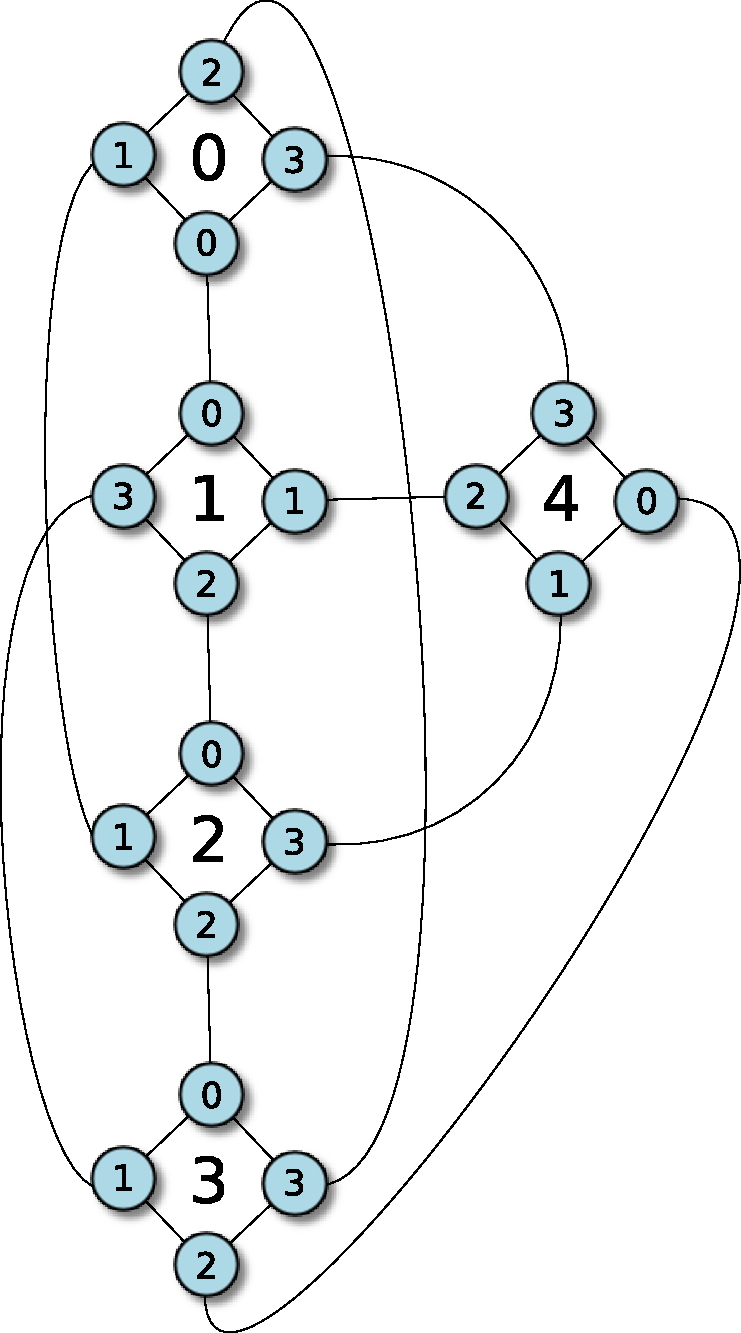
\includegraphics[width=.59\textwidth]{../pics/3-7-replacement-024-0123413}
      \caption{$K_5 \protect\replacement C_4$}
      \label{fig:replacement}
    \end{figure}
  \end{columns}
\end{frame}




\section{The Zig-Zag Product}

\begin{frame}{Definition: The Zig-Zag Product}
\begin{definition}
\label{def:zig_zag:old}
The {\bf zig-zag} product of $G$ (with a given enumeration $\Enum$) with $H$, denoted $G \zigzag H$, is a graph with vertex set $V(G) \times V(H)$ for which $\left( u, a \right)$ is adjacent to $ \left( v, b \right)$ if and only i
\begin{enumerate}
  \item $\left(u,v\right) \in \edgeS{G}$
  \item both $\left(a, \enum_{u}(v) \right)$ and $\left(\enum_{v}(u), b\right)$ are in $\edgeS{H}$
\end{enumerate}
\end{definition}
\begin{figure}[h]
  \centering
  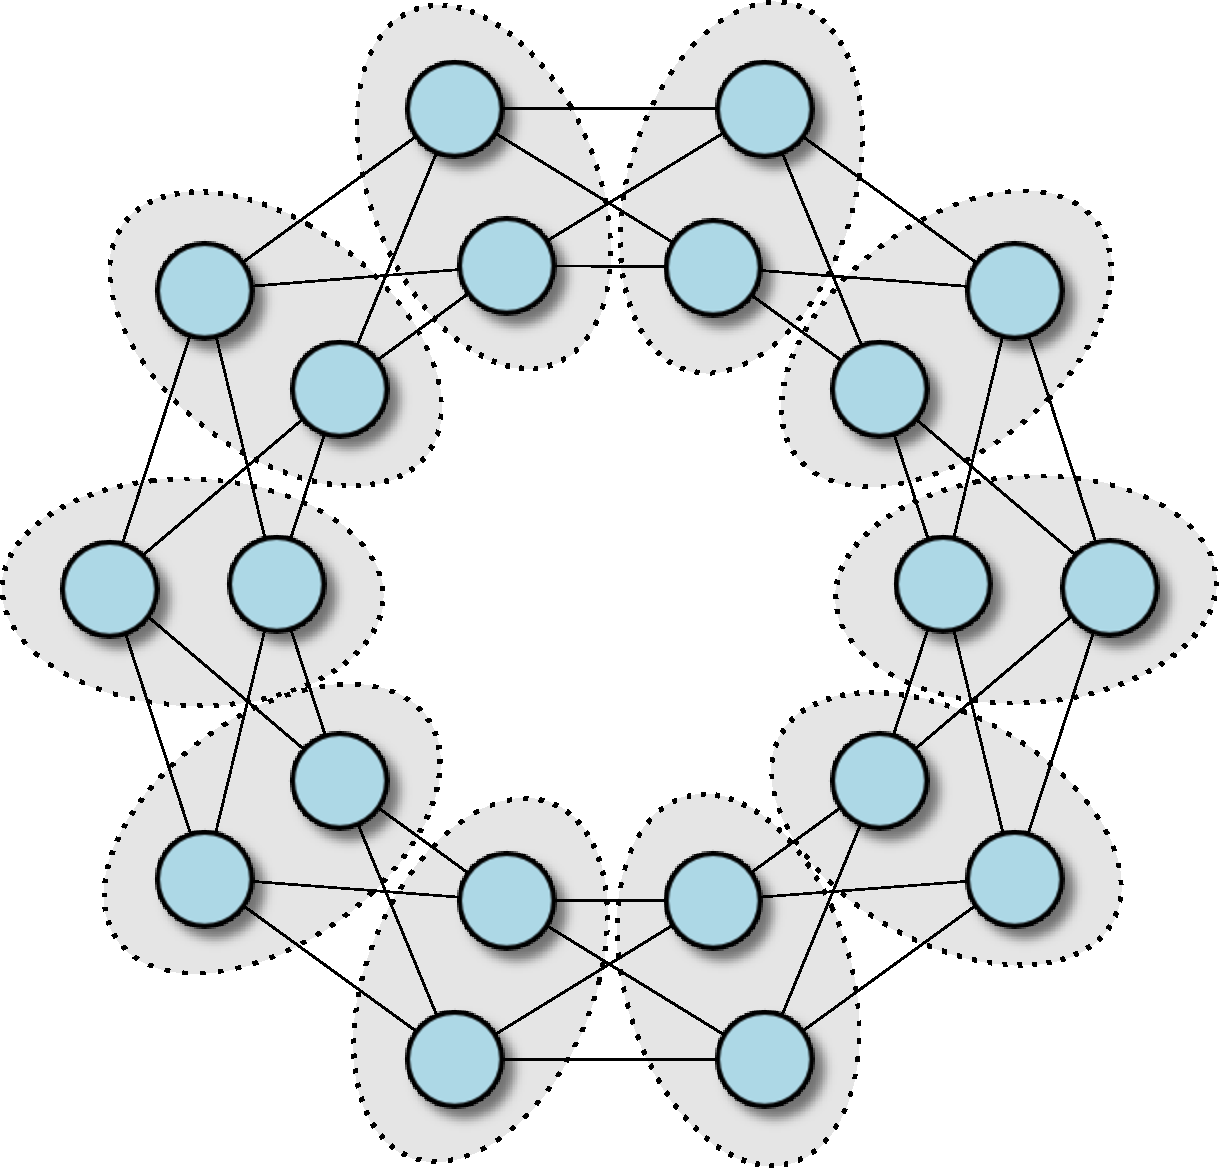
\includegraphics[height=.35\textheight]{../pics/10-zigzag}
  \caption{Example of $K_5 \protect\zigzag C_4$ }
  \label{fig:zigzag_ex}
\end{figure}

\end{frame}


\begin{frame}{Relationship to Replacement Product}
The {\em zig-zag} product is the graph whose adjacency's arise from walks of length three of a ``zig-zag'' nature in $G \replacement H$.
\begin{enumerate}
\item<2-> An edge within one {\em cloud} (zig).
\item<3-> An edge connecting one {\em cloud} to another (zag).
\item<4-> An edge within the final {\em cloud} (zig again).
\end{enumerate} 


\begin{figure}[h!]
\centering
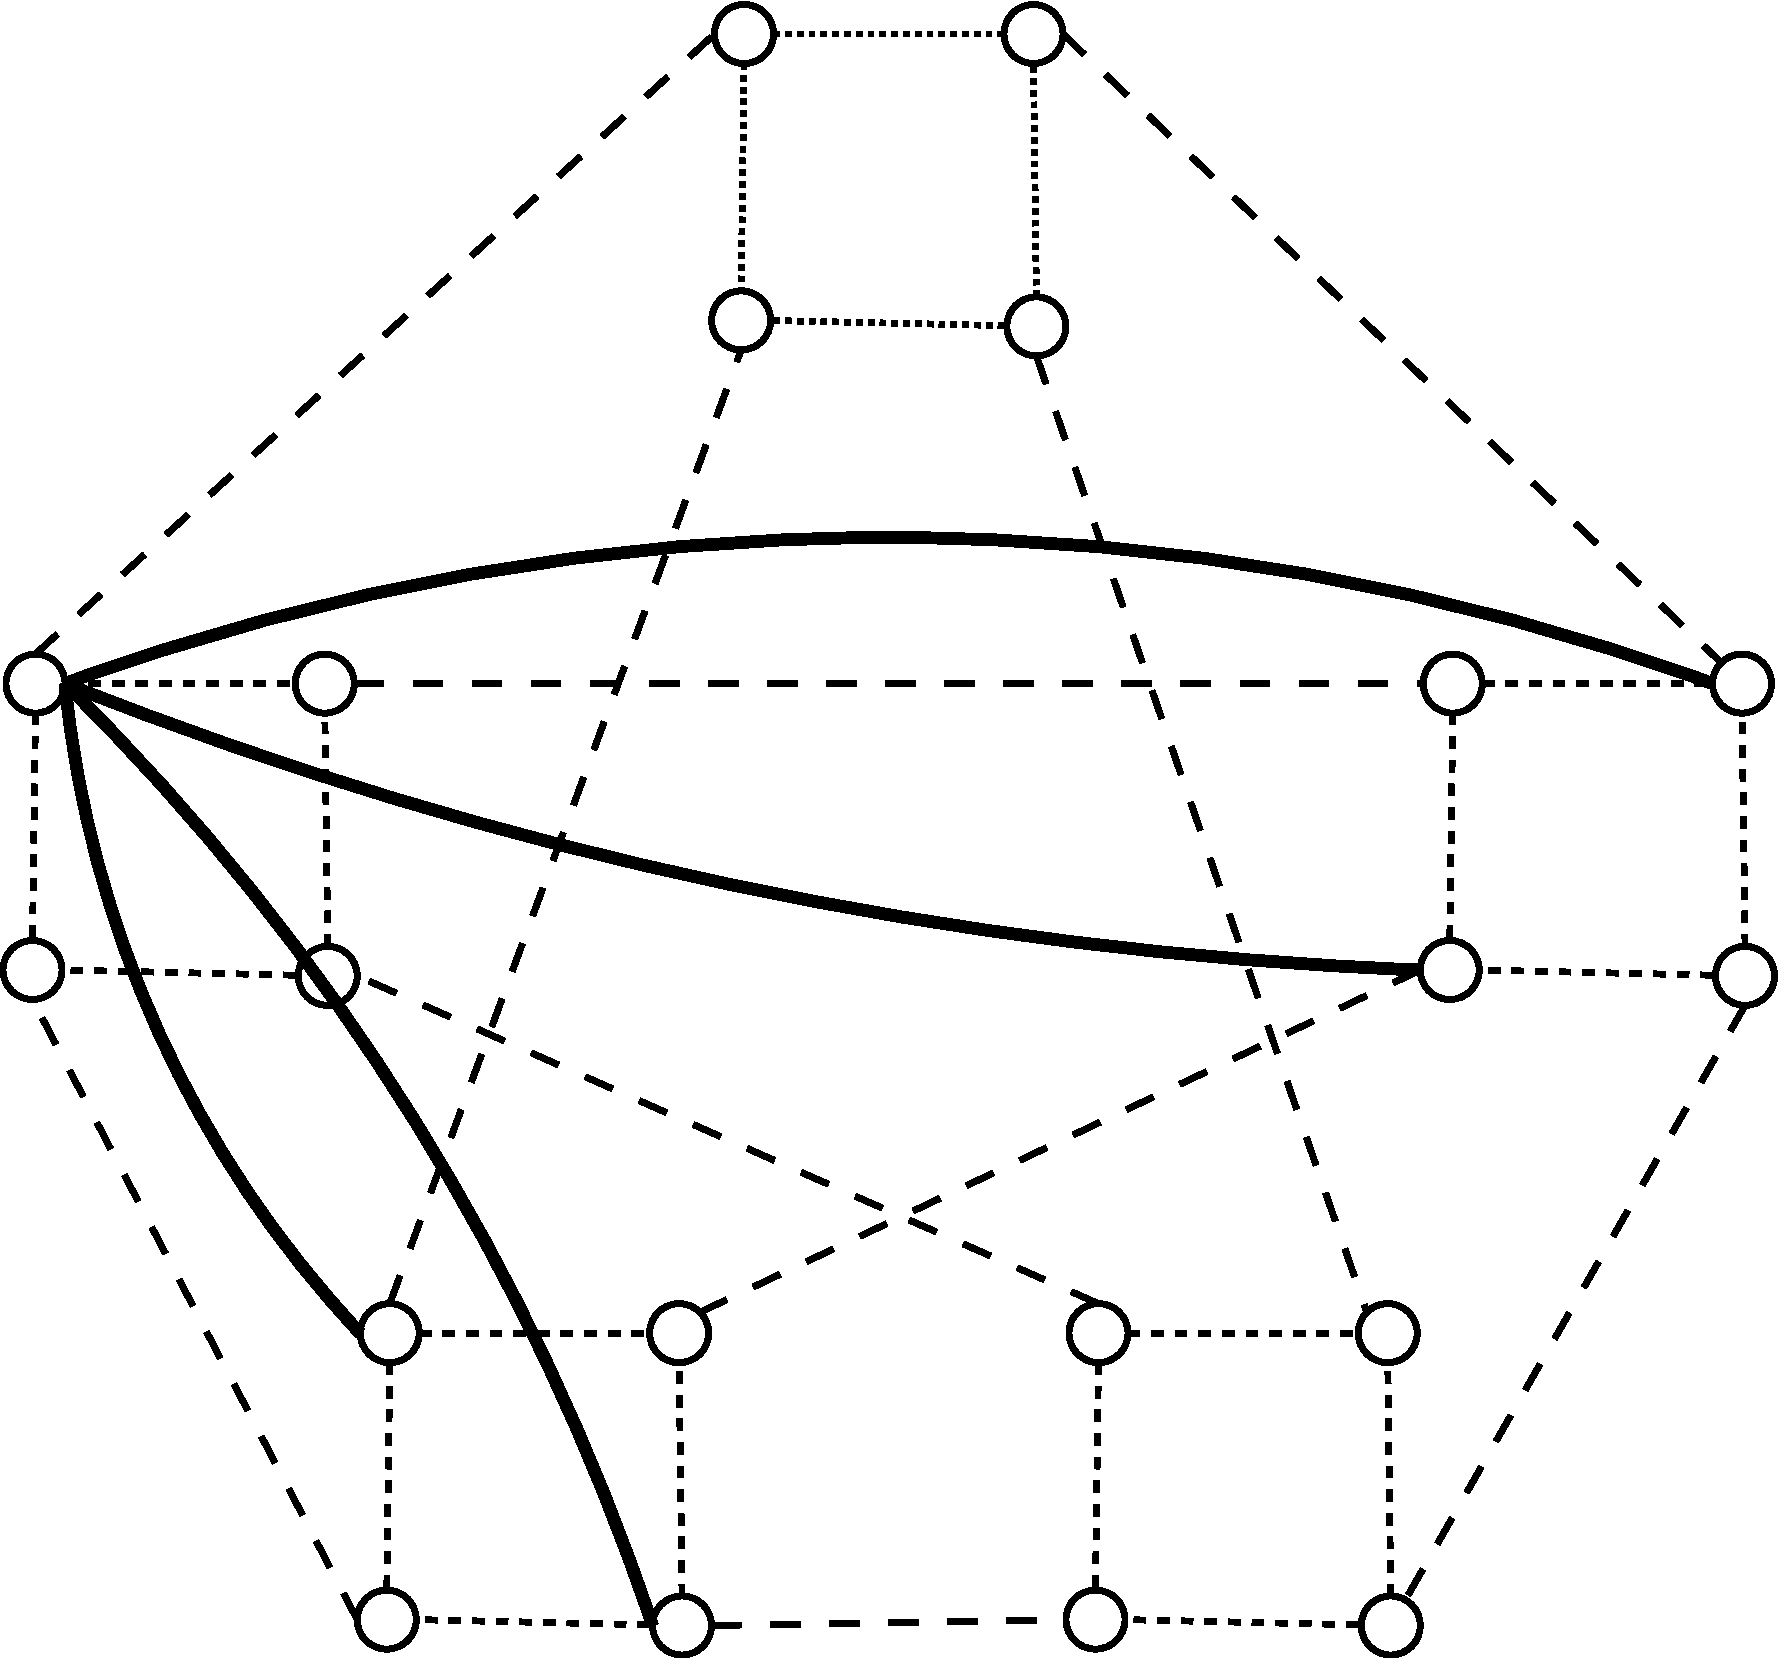
\includegraphics[height=.30\textheight]{../pics/zig_zagK5_C4}
\caption{``zig-zag'' edges incident in $K_5 \protect\replacement C_4$}
\end{figure}
\noindent

\end{frame} 

\begin{frame}{Zig-Zag Product and RP-Isomorphisms}
  \begin{theorem}
\label{def:isomorphic_replacement:zigzag}
If $G \replacement H$ and  $G \replacement^{\prime} H$ are rp-isomorphic. Then $G \zigzag H$ is isomorphic to $G \zigzag^{\prime} H$.
\end{theorem}

\begin{figure}[h!]
\centering
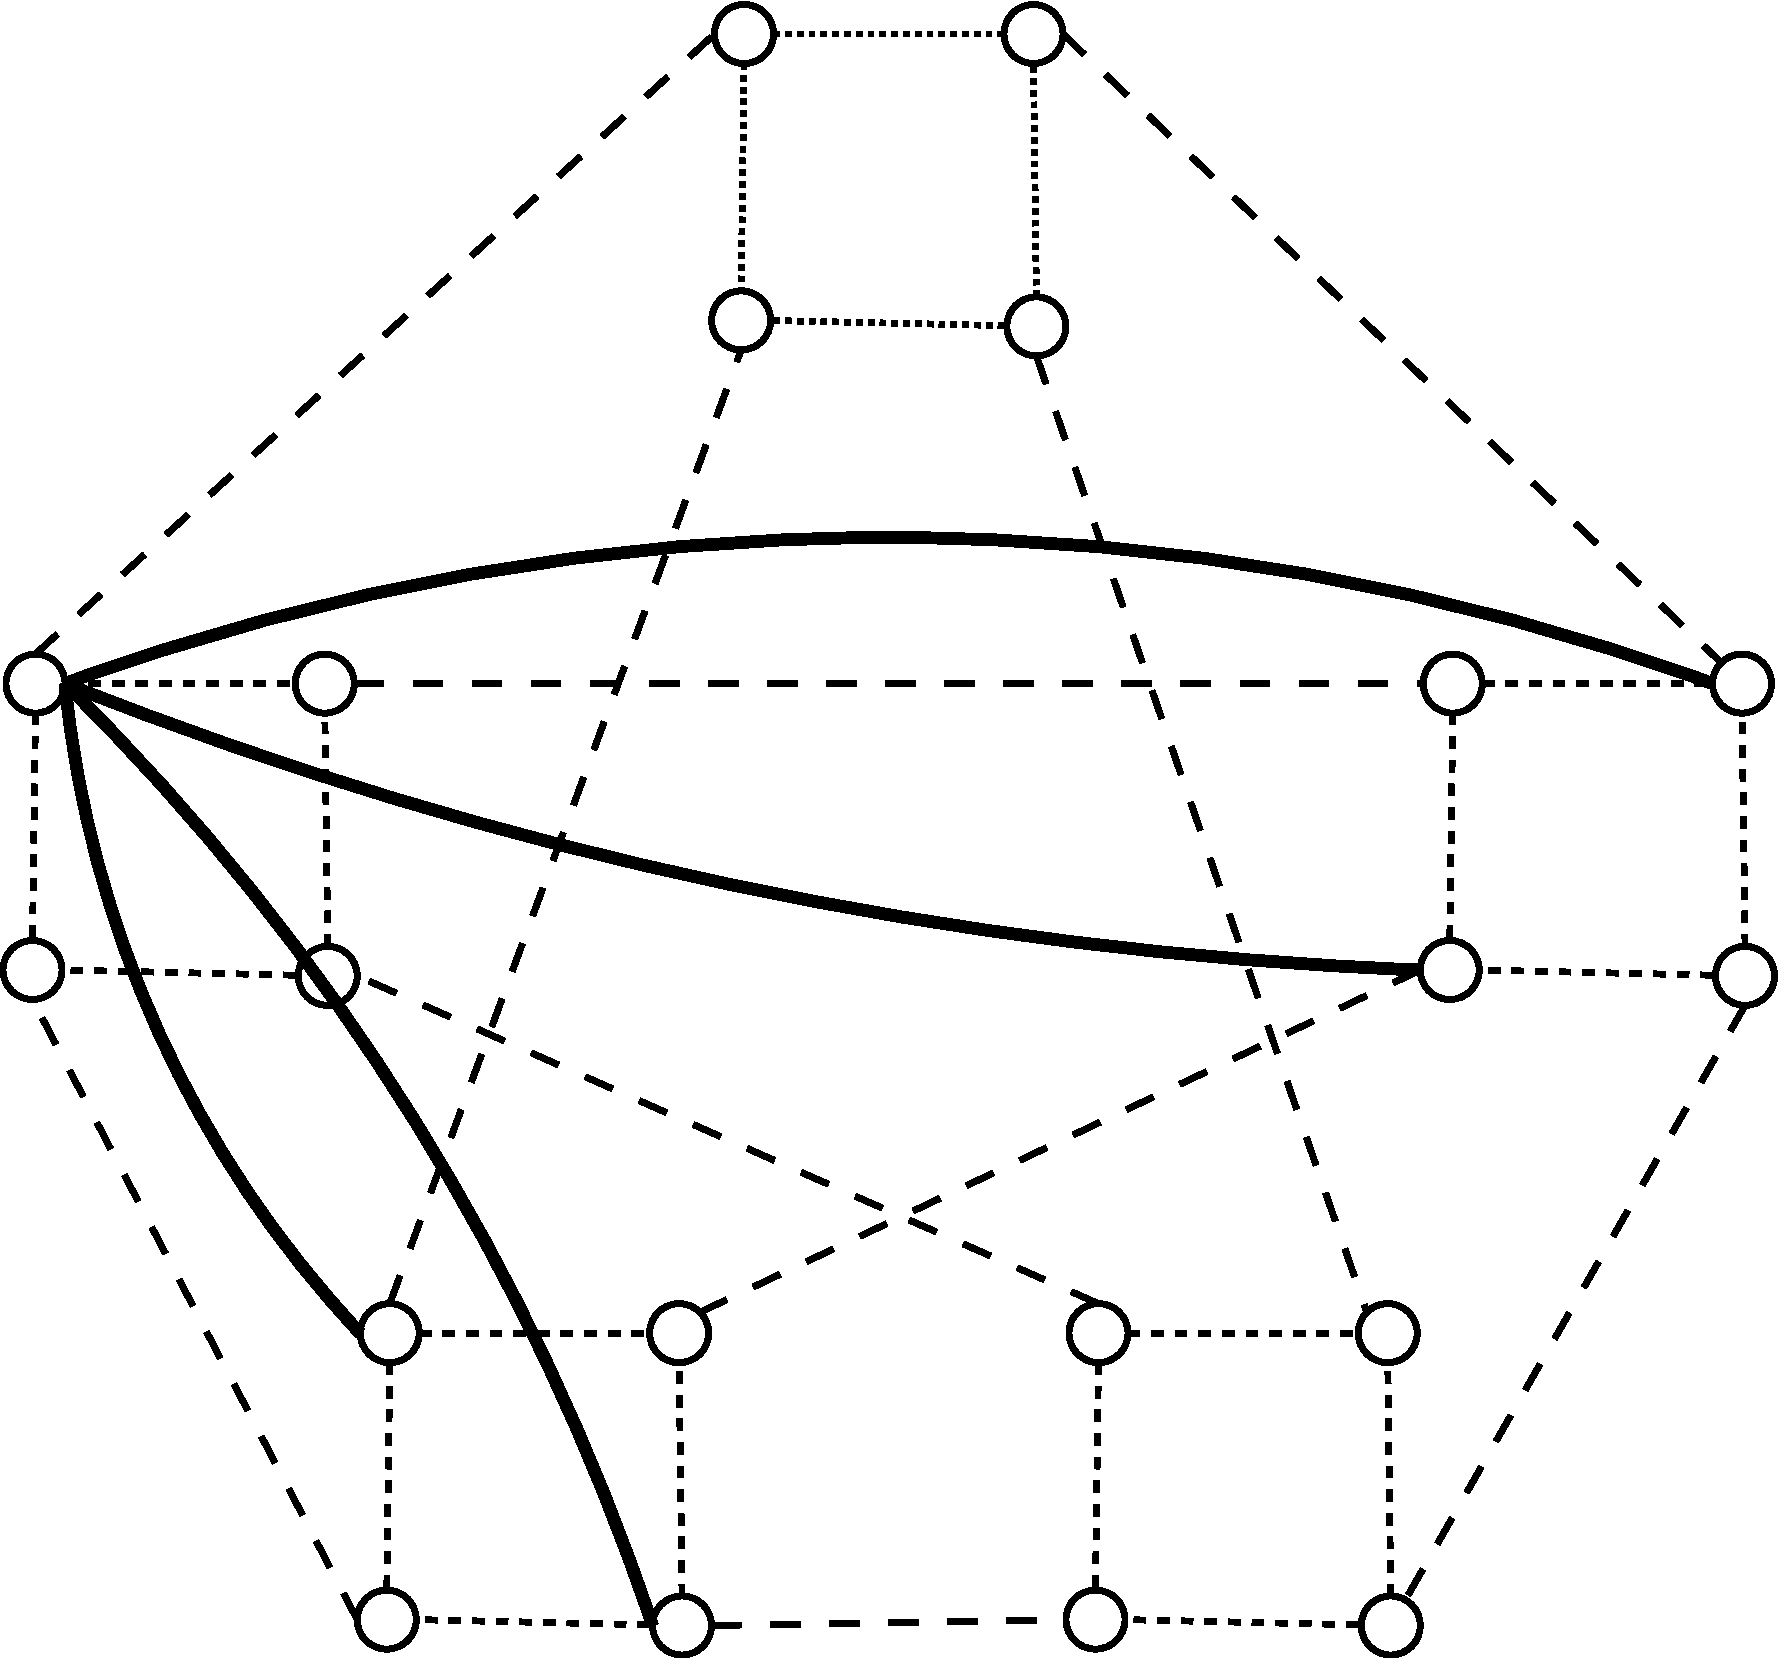
\includegraphics[height=.30\textheight]{../pics/zig_zagK5_C4}
\caption{``zig-zag'' edges incident in $K_5 \protect\replacement C_4$}
\end{figure}
\end{frame}

\begin{frame}{The size of rp-isomorphism classes:}

\begin{theorem}
\label{thm:upperbound_iso}
  Let $n( G \replacement H)$ be the number of unique non-isomorphic replacement products. Then we have \[ n(G \replacement H) \leq \left(\frac{m!}{\left| \Aut(H)\right|}  \right)^{n}  \]
\end{theorem}


\begin{corollary}
  Let $G$ be any $3$-regular graph on $n$-vertices and consider the cycle graph on three vertices $C_3$. Then  \[  n(G \replacement C_3 ) \leq \left( \frac{ 3! }{ \card{D_3}} \right)^n = \left( \frac{6}{6} \right)^n = 1    \]
\end{corollary}
  
\uncover<2->{{\small {\bf Note:} The smallest ``interesting example'' has to be $4$-regular}}
\end{frame}
\part{Classification of $K_5 \protect \replacement C_4$ and $K_5 \protect \zigzag C_4$}
\begin{frame}{Classification of $K_5 \protect \replacement C_4$ and $K_5 \protect \zigzag C_4$}
\begin{quote}
The art of doing mathematics consists in finding that special case which contains all the germs of generality. {\bf -David Hilbert}
\end{quote}

  \begin{figure}[h]
    \centering
    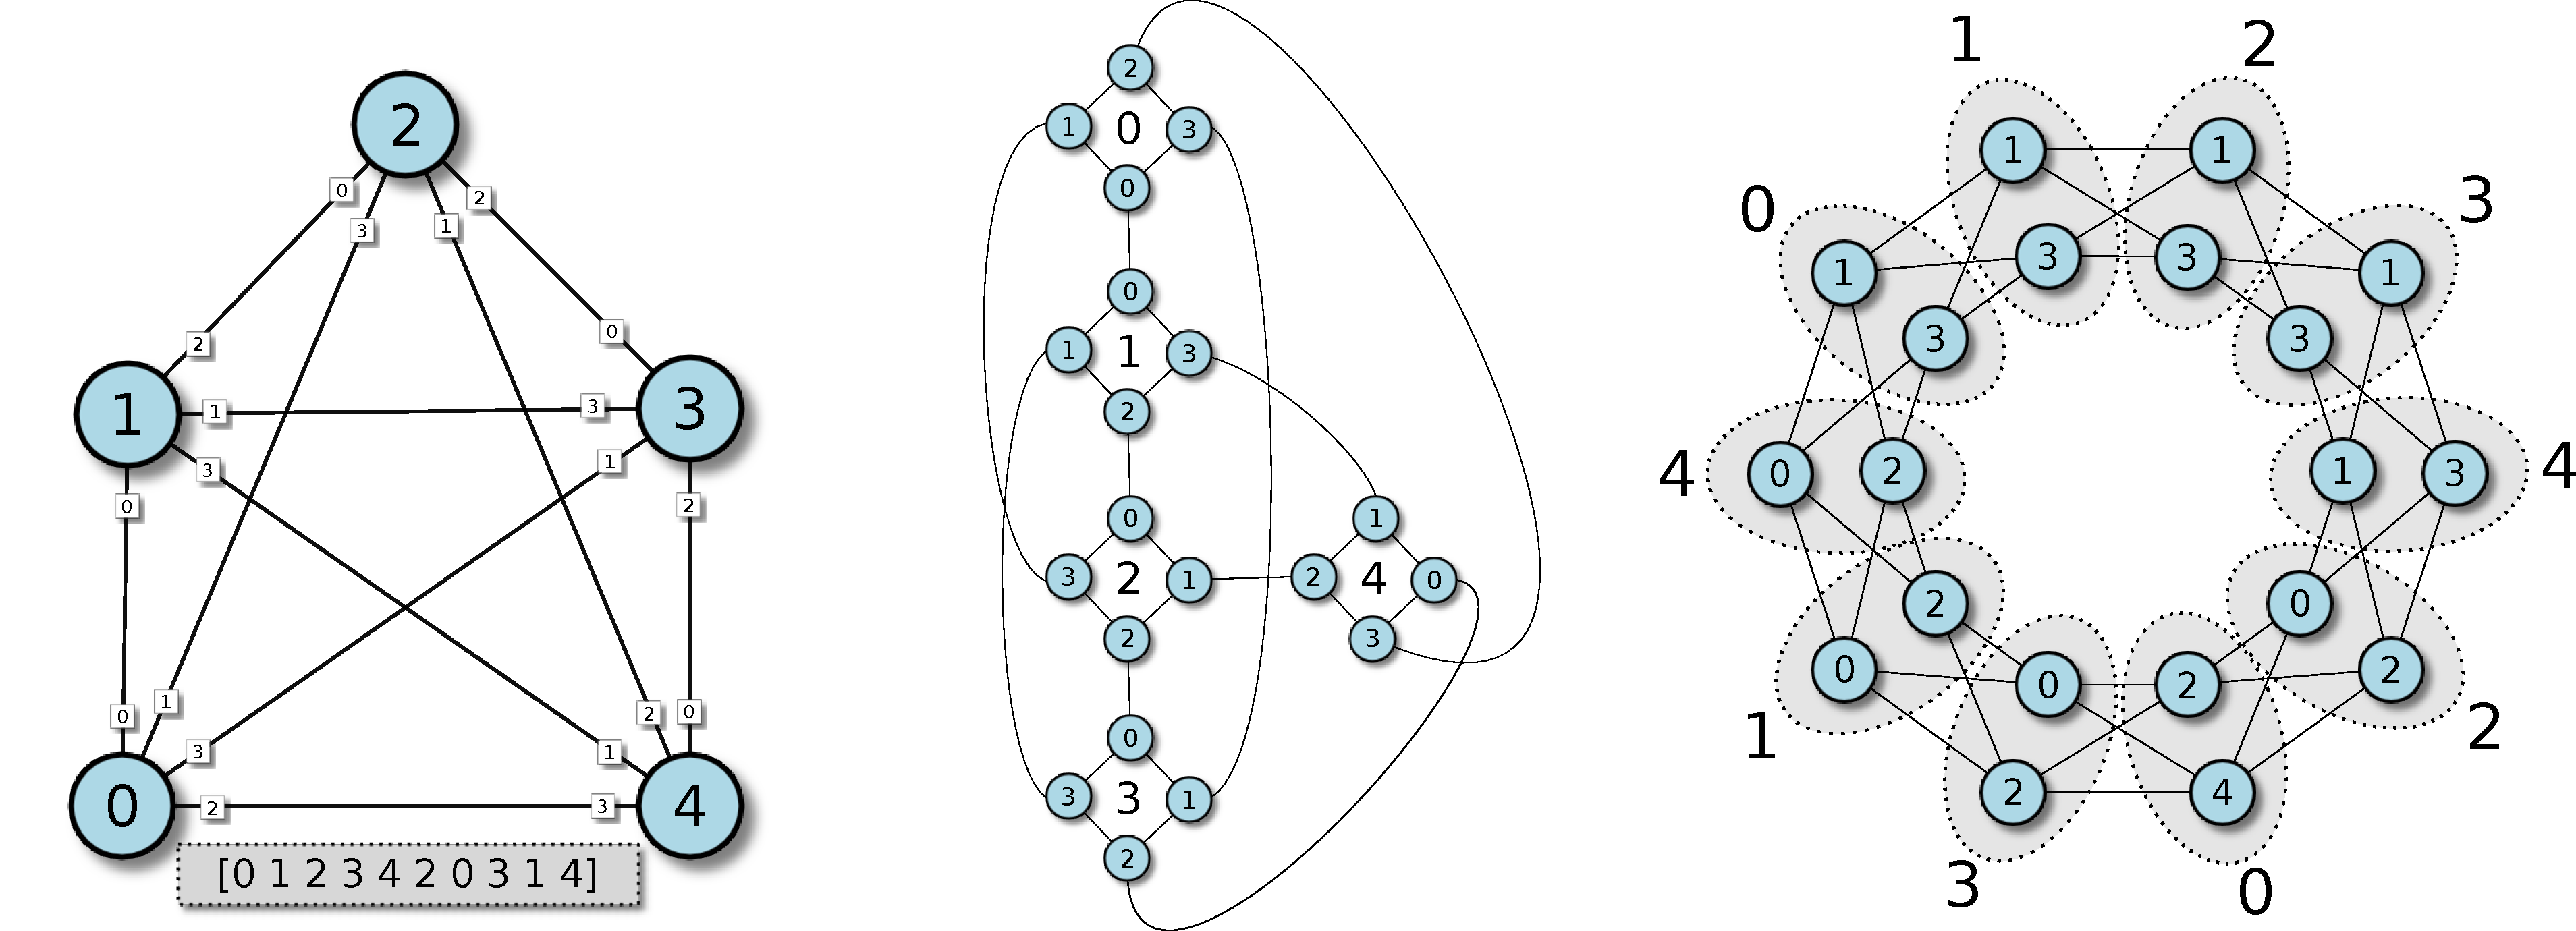
\includegraphics[height=.30\textheight]{../pics/10-example}
    \caption{Example of an enumeration of $K_5$ and the associated zig-zag and replacement products.}
    \label{fig:10-example}
  \end{figure}

  
\end{frame}

\begin{frame}{$K_5 \protect\zigzag C_4$}
  \begin{block}{Early Experiments}
    Led us to graphs which all shared a very similar structure, but with intriguing differences. 
  \end{block}
  \begin{columns}
    \column{.33\textwidth}
    \begin{figure}[h]
      \centering
        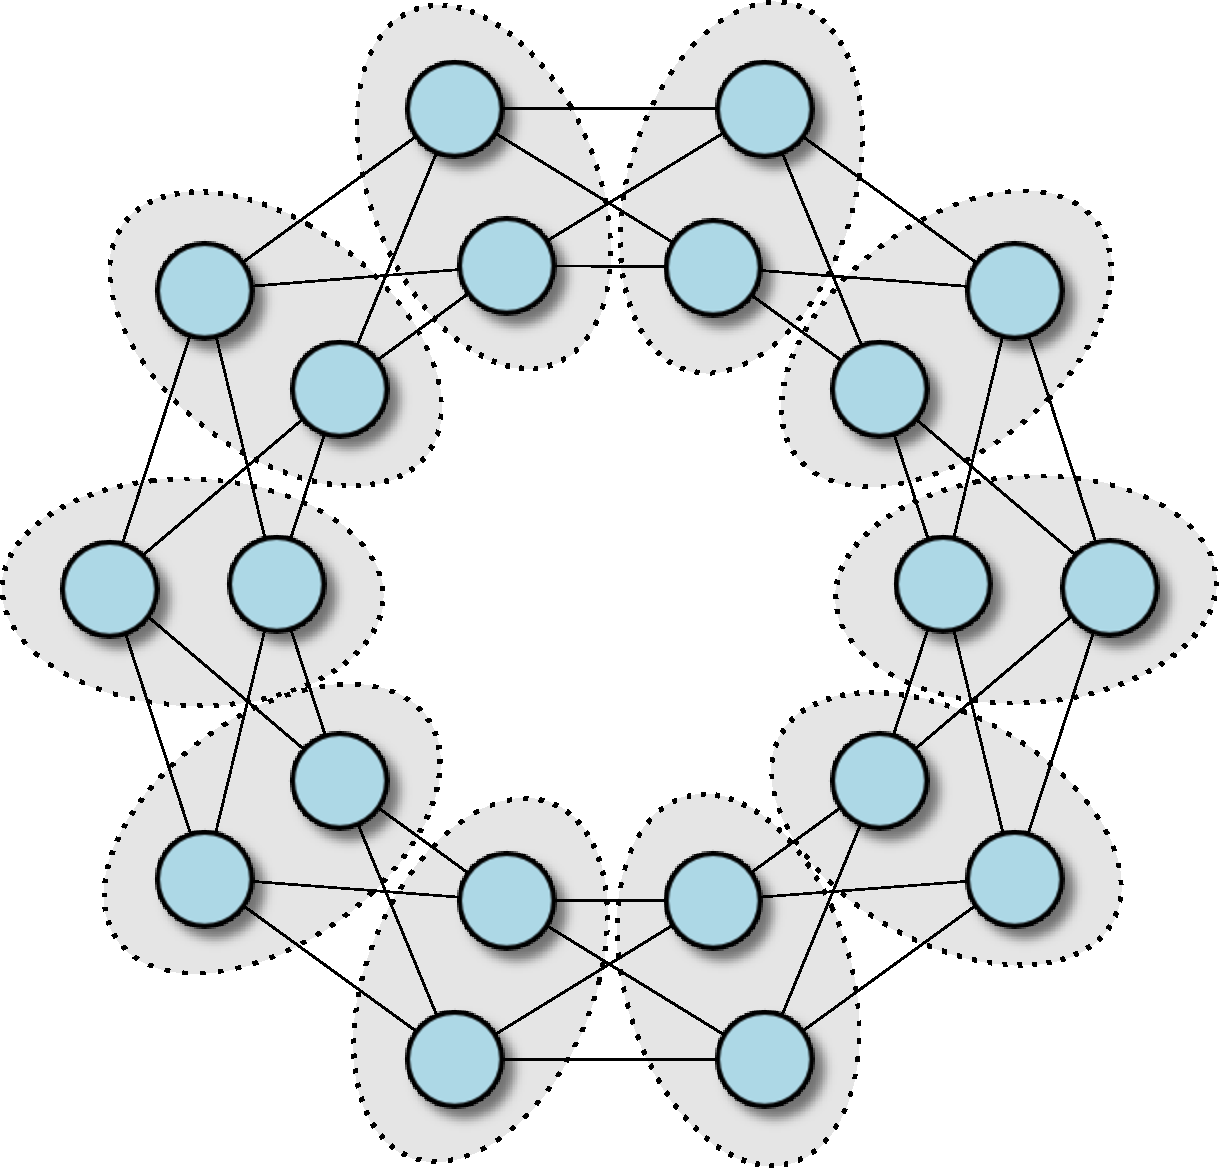
\includegraphics[width=.80\textwidth]{../pics/10-zigzag}
      \caption{$K_5 \protect\zigzag C_4$}
      \label{fig:10zigzag}
    \end{figure}
    \column{.33\textwidth}
    \begin{figure}[h]
      \centering
        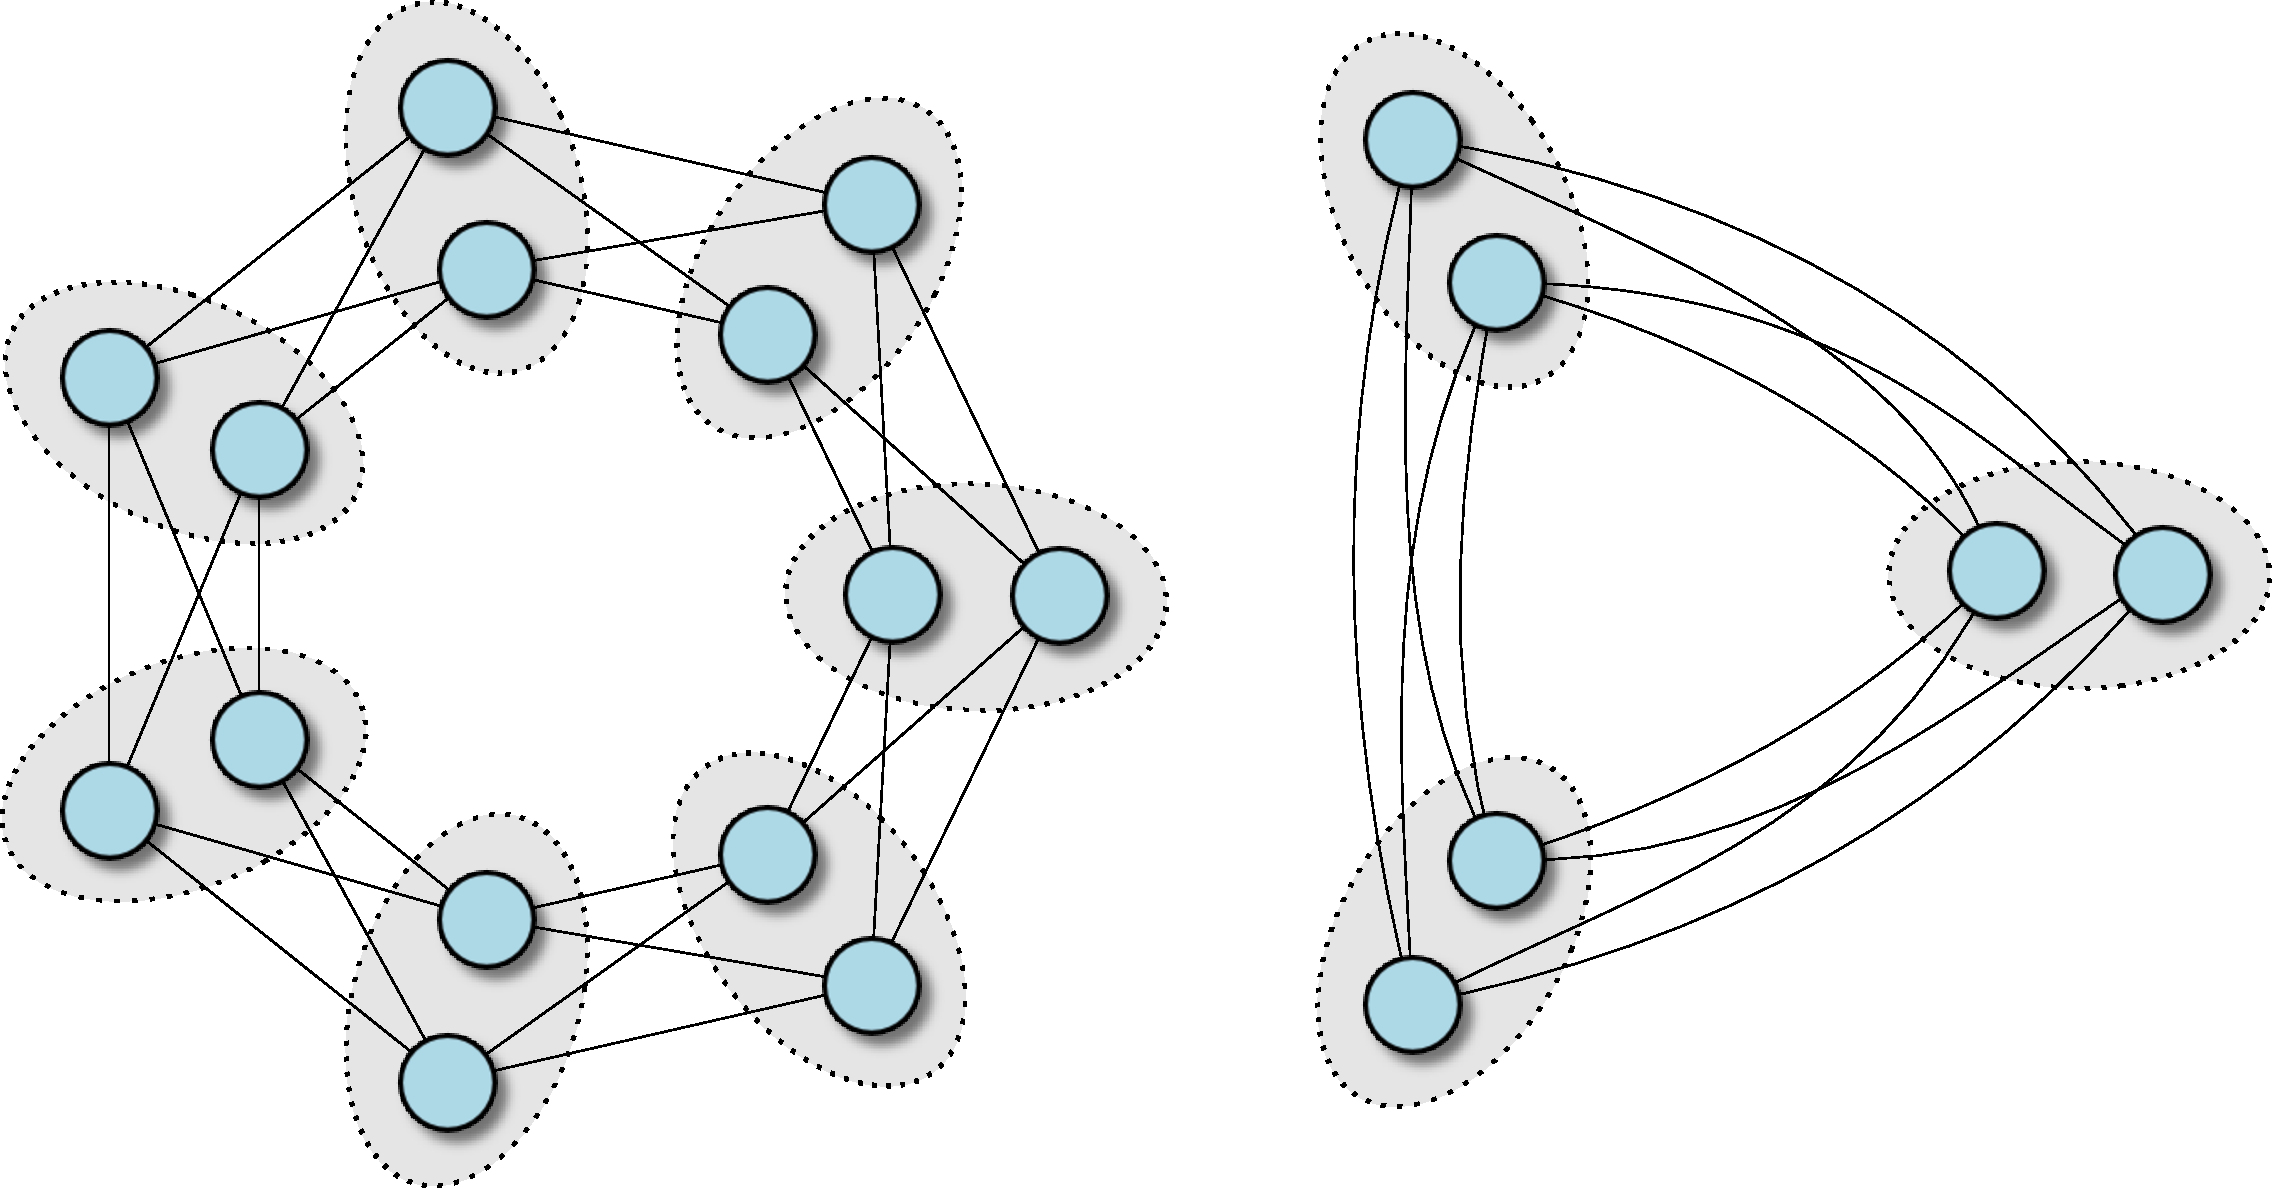
\includegraphics[width=1.0\textwidth]{../pics/3-7-zigzag}
      \caption{$K_5 \protect\zigzag C_4$}
      \label{fig:10zigzag}
    \end{figure}
    \column{.33\textwidth}
    \begin{figure}[h]
      \centering
        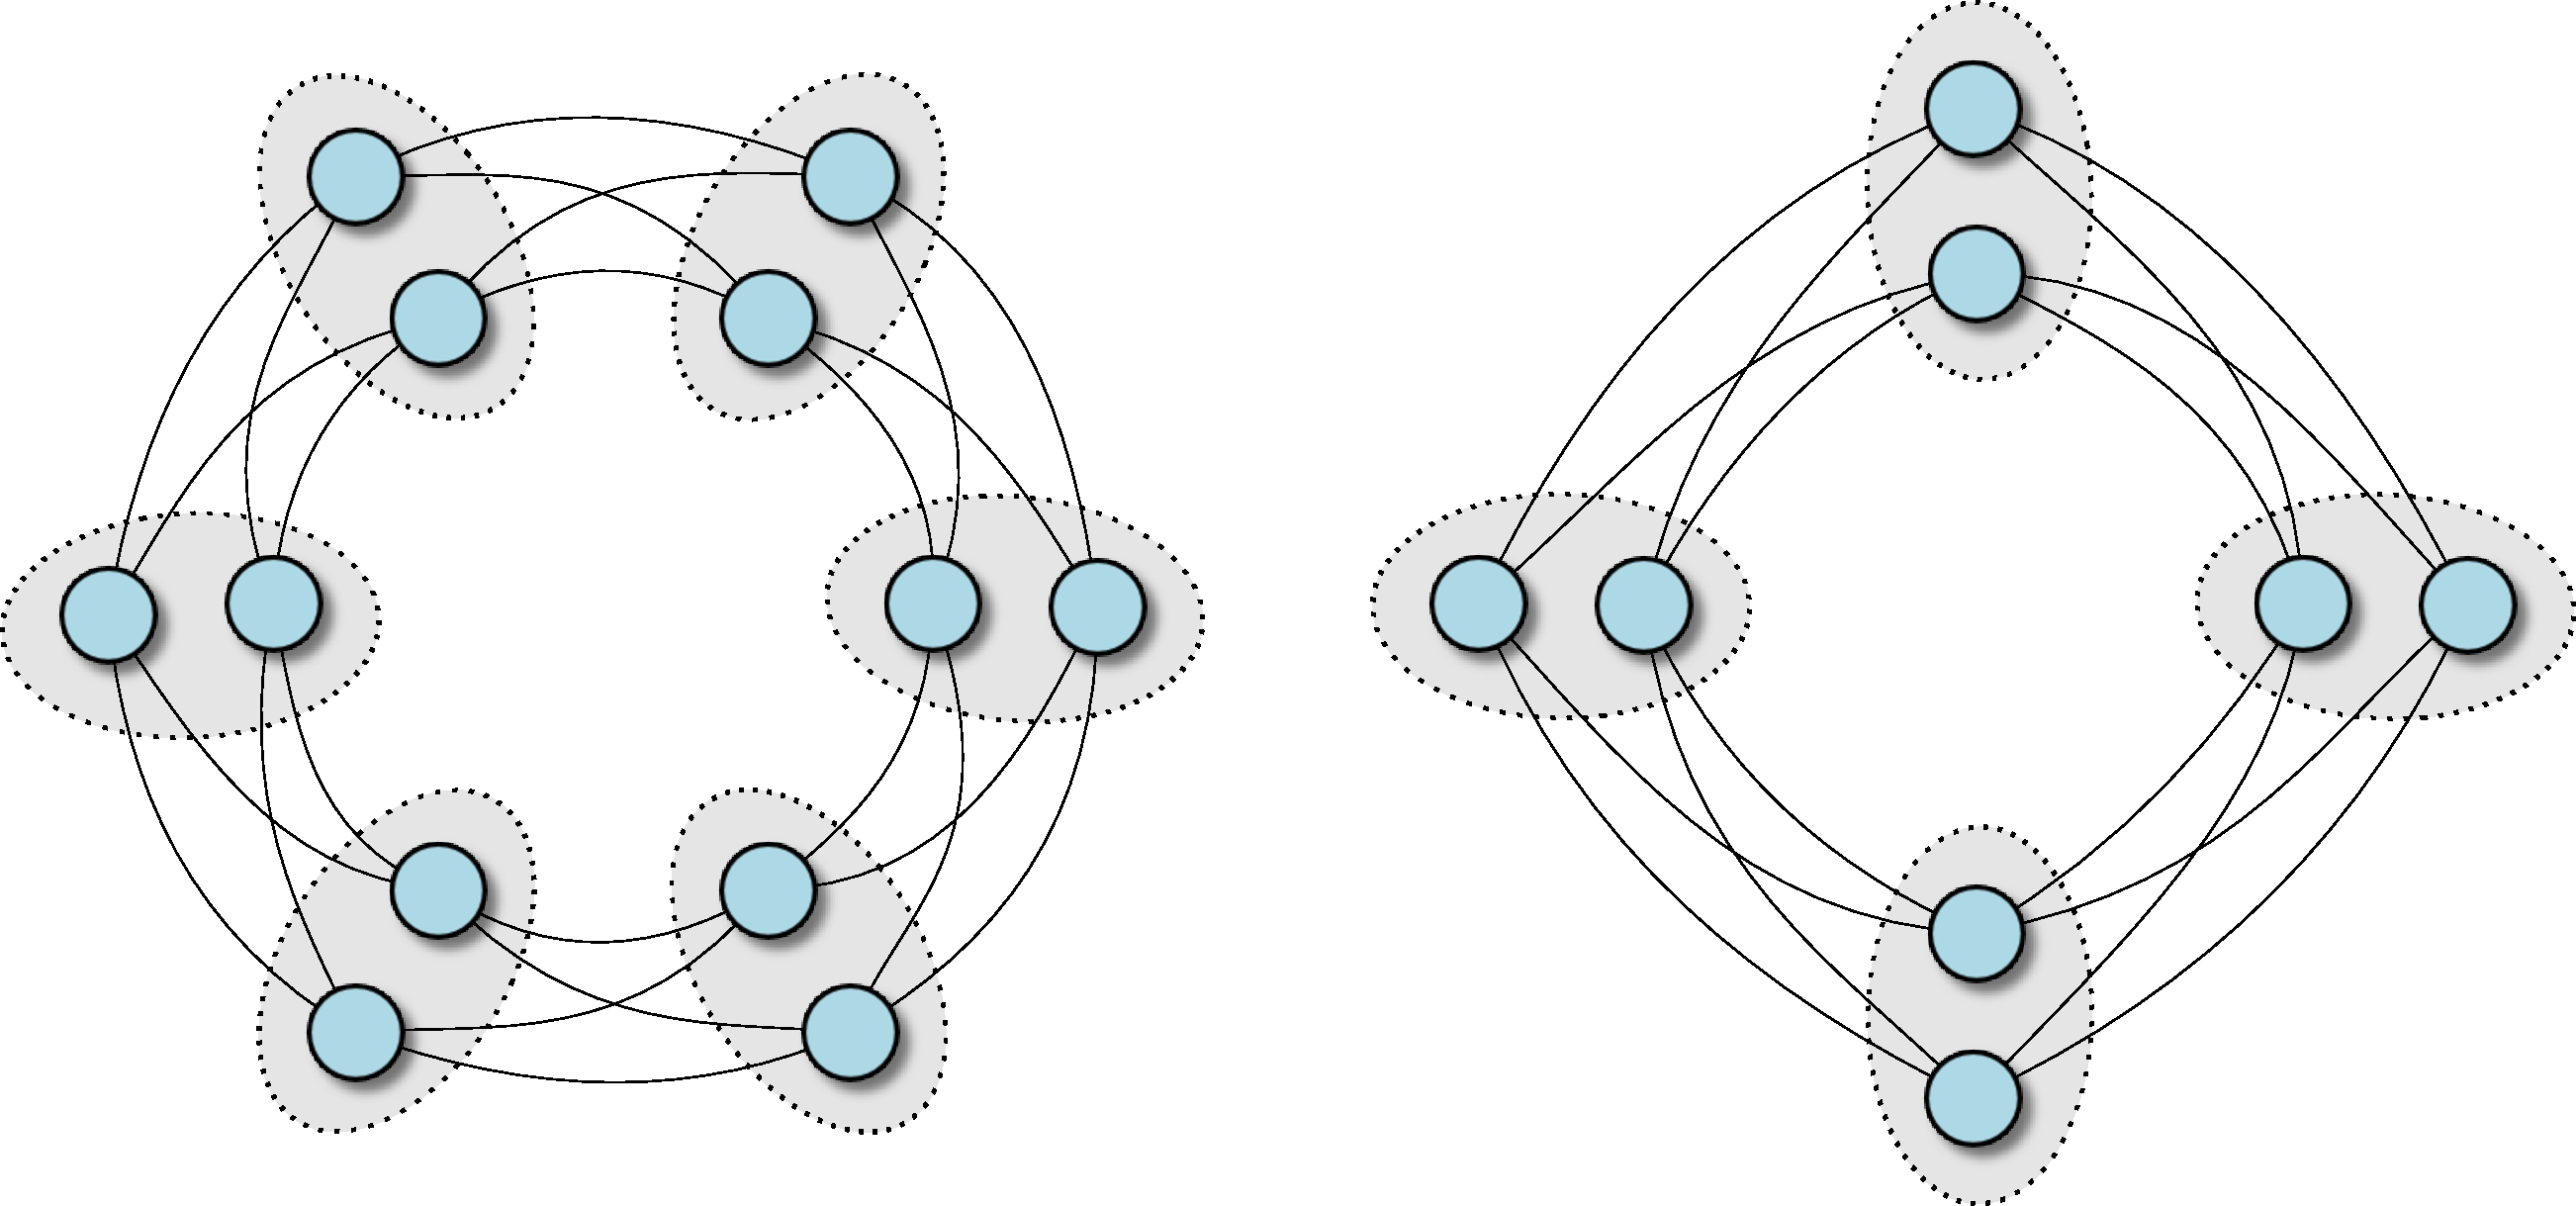
\includegraphics[width=1.00\textwidth]{../pics/4-6-zigzag}
      \caption{$K_5 \protect\zigzag C_4$}
      \label{fig:10zigzag}
    \end{figure}
  \end{columns}
\end{frame}

\begin{frame}{$K_5 \protect\zigzag C_4$ and $K_5 \protect\replacement C_4$}
  \begin{figure}[h]
    \centering
      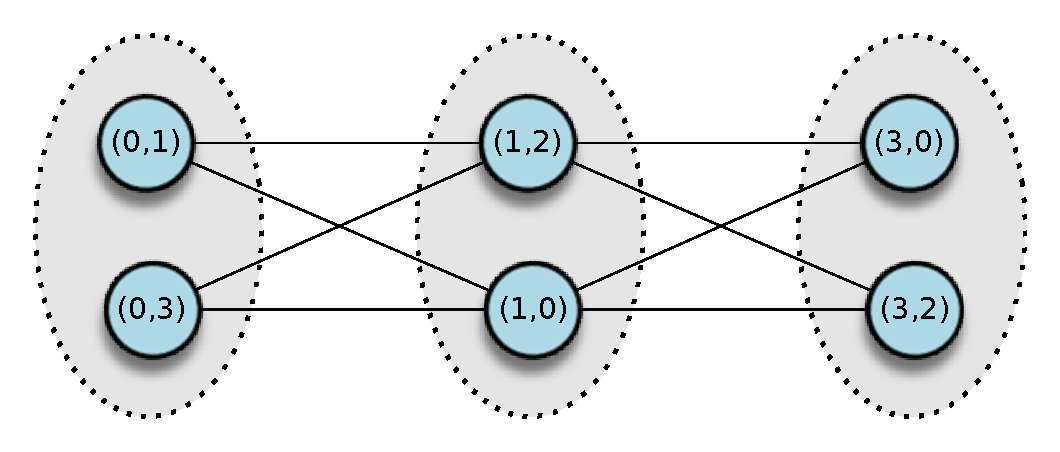
\includegraphics[width=.65\textwidth]{../pics/zig-zag-nhbd-example}
    \caption{Example neighborhood in $K_5 \protect\zigzag C_4$}
    \label{fig:exzznhbd}
  \end{figure}

\uncover<2->{
  \begin{figure}[h]
    \centering
      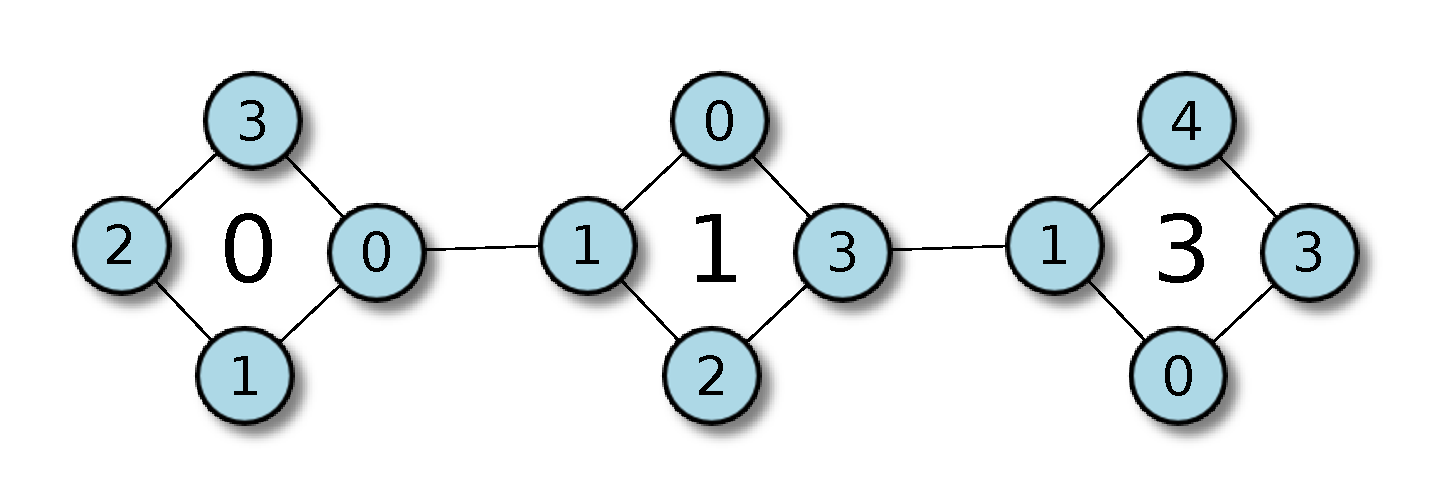
\includegraphics[width=.645\textwidth]{../pics/replacement-neighborhood}
    \caption{Corresponding neighborhood in $K_5 \protect\replacement C_4$}
    \label{fig:replacementnhdb}
  \end{figure}
}


\end{frame}


\begin{frame}{$K_5 \protect\replacement C_4$ and $K_5$}
  \begin{columns}
    \column{.50\textwidth}
    \begin{figure}[h]
      \centering
      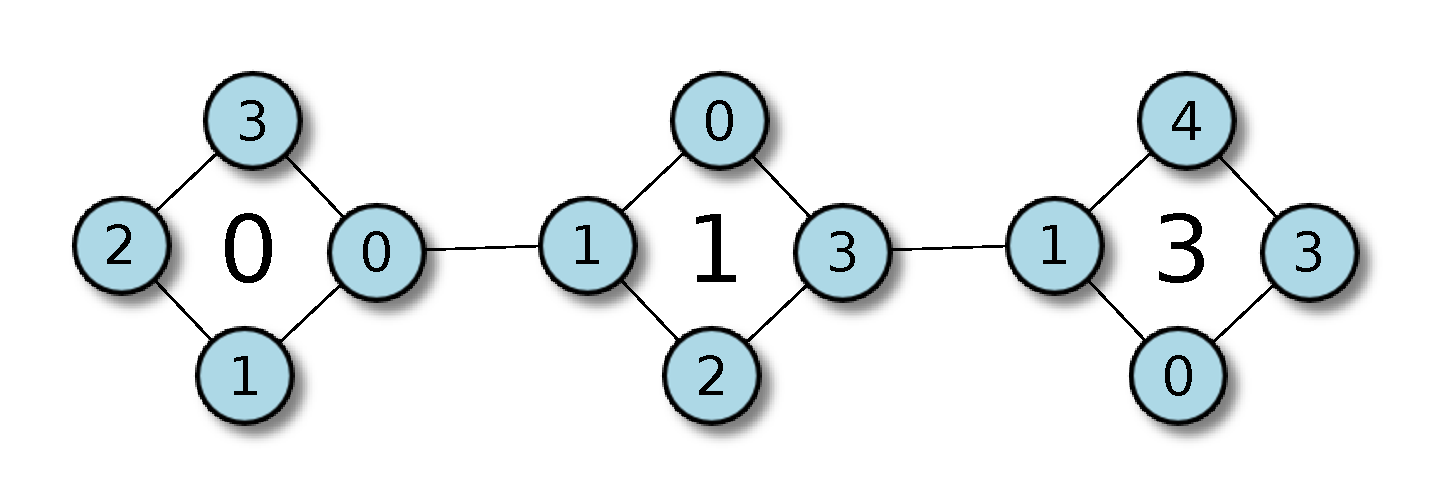
\includegraphics[width=.80\textwidth]{../pics/replacement-neighborhood}
      \caption{Neighborhood in $K_5 \protect\replacement C_4$}
      \label{fig:replacementnhdb}
    \end{figure}
    \column{.50\textwidth}
    \uncover<2>{  
      \begin{figure}[h]
        \centering
        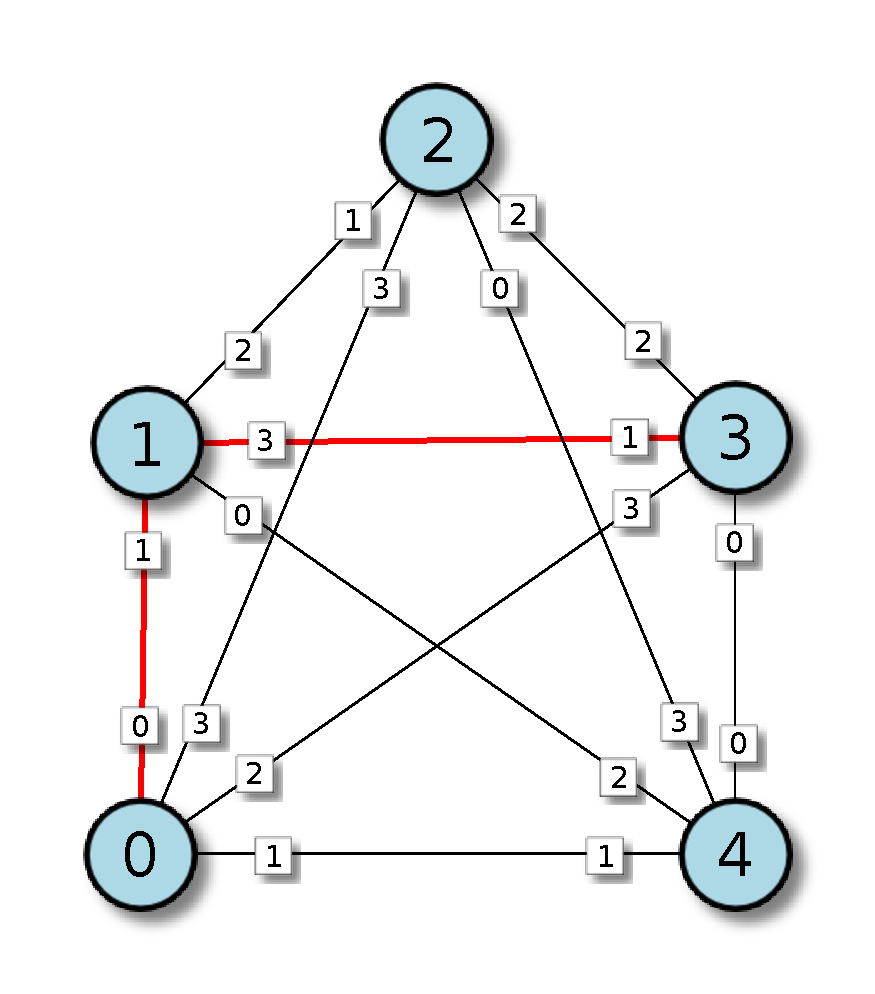
\includegraphics[width=.80\textwidth]{../pics/ppath}
        \caption{Corresponding Path in $K_5$}
        \label{fig:K5ppath}
      \end{figure}
    }
  \end{columns}
\end{frame}

\begin{frame}{$K_5$ and {\em parity}}
  \begin{columns}
    \column{.50\textwidth}
    \begin{block}{Observation:}
      \begin{itemize}
        \item Neighborhoods in $K_4 \zigzag C_4$ correspond to paths in $K_5$
        \item Paths which {\em enter} and {\em leave} by edges labeled with the same \alert{parity}
      \end{itemize}
       
    \end{block}
    \column{.50\textwidth}
    \uncover<1->{  
      \begin{figure}[h]
        \centering
        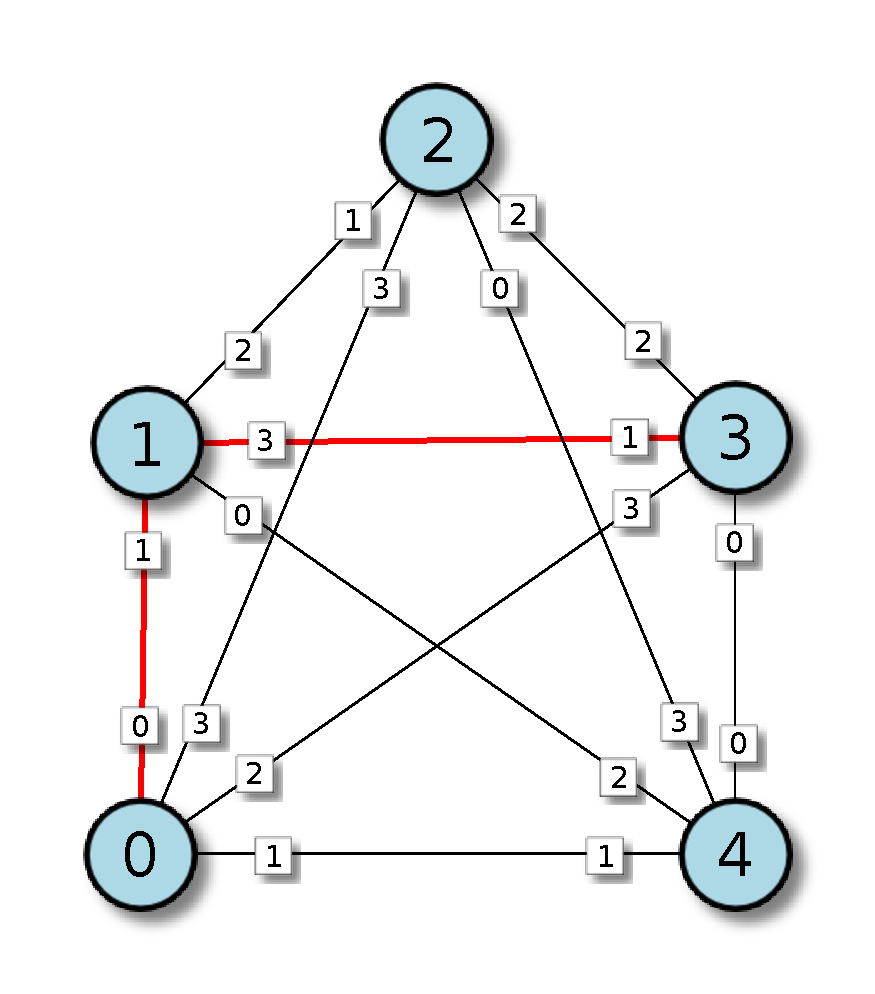
\includegraphics[width=.80\textwidth]{../pics/ppath}
        \caption{Corresponding Path in $K_5$}
        \label{fig:K5ppath}
      \end{figure}
    }
  \end{columns}
\end{frame}

\section{Parity Circuit Decompositions (PCDS)}
\begin{frame}{Parity Circuits in $K_5$}

\begin{definition}
  \label{def:pcircuit}
    Let $\ppath = \left[ u_1\  u_2\  \cdots\  u_k \right]$ be a closed walk on $K_5$ with enumeration $\Enum$. $\ppath$ is a {\bf parity circuit } of length $k$ if both 
    \begin{itemize}
      \item For each $u_{i} \in \ppath$,  $\enum_{u_i}( u_{i-1}) = \enum_{u_{i}}(u_{i+1}) \pm 2 \bmod{4}$. 
      \item No edge is traversed more than once. 
      \end{itemize} 
\end{definition}
\begin{columns}
  \column{.50\textwidth}
  \begin{figure}[h]
    \centering
    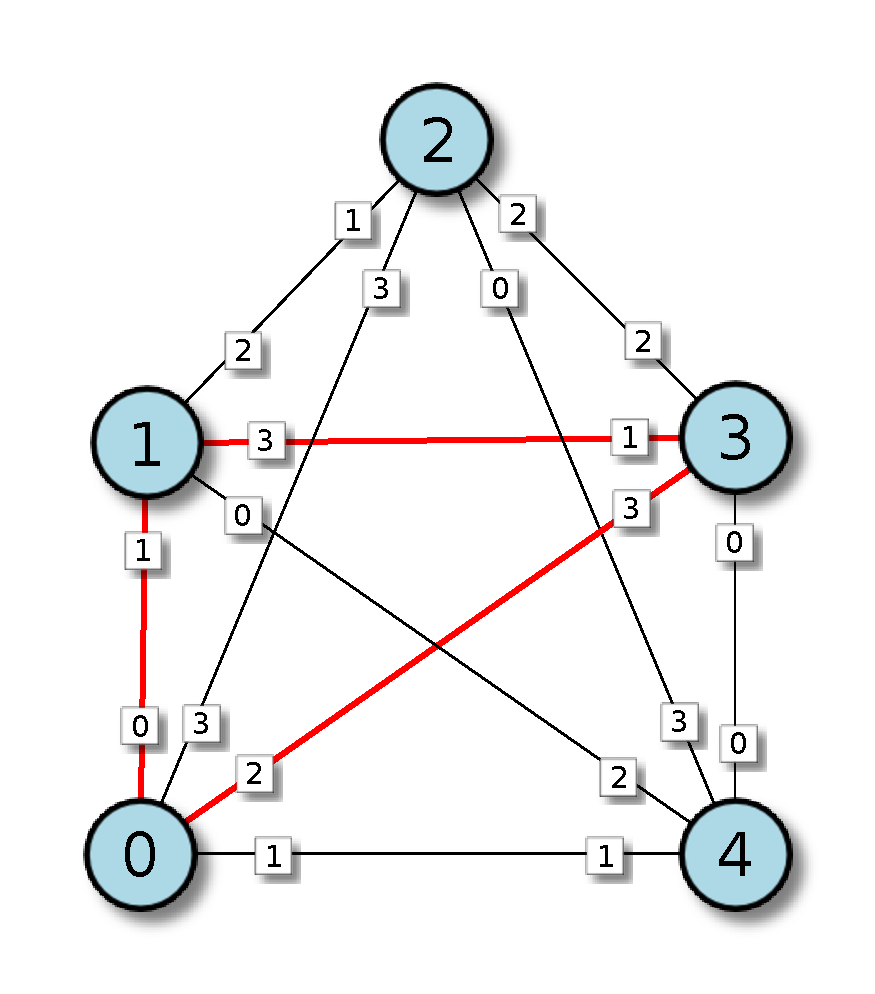
\includegraphics[height=.43\textheight]{../pics/3-pcircuit}
    \caption{Parity circuit of length $3$}
    \label{fig:K5ppath}
  \end{figure}
  \column{.50\textwidth}
  \begin{itemize}
    \item Parity Circuit \textcolor{red}{$\left[0 \ 1\ 3 \right]$} 
  \end{itemize}
\end{columns}

\end{frame}

\begin{frame}{Parity Circuits in $K_5$}
  \begin{columns}
    \column{.50\textwidth}
    \begin{itemize}
      \item<1-> The compliment (edgewise) of \textcolor{red}{$\left[0 \ 1 \ 3 \right]$} leaves edges of the opposite parity.
      \item<2-> \textcolor{green}{$\left[0\ 2\ 1\ 4\ 3\ 2\ 4 \right]$} is a parity circuit of length $7$
      \item<3-> \textcolor{red}{$\left[0 \ 1 \ 3 \right]$}\textcolor{green}{$\left[0\ 2\ 1\ 4\ 3\ 2\ 4 \right]$}
    \end{itemize}
    \column{.50\textwidth}
    \only<1>{
      \begin{figure}[h]
        \centering
          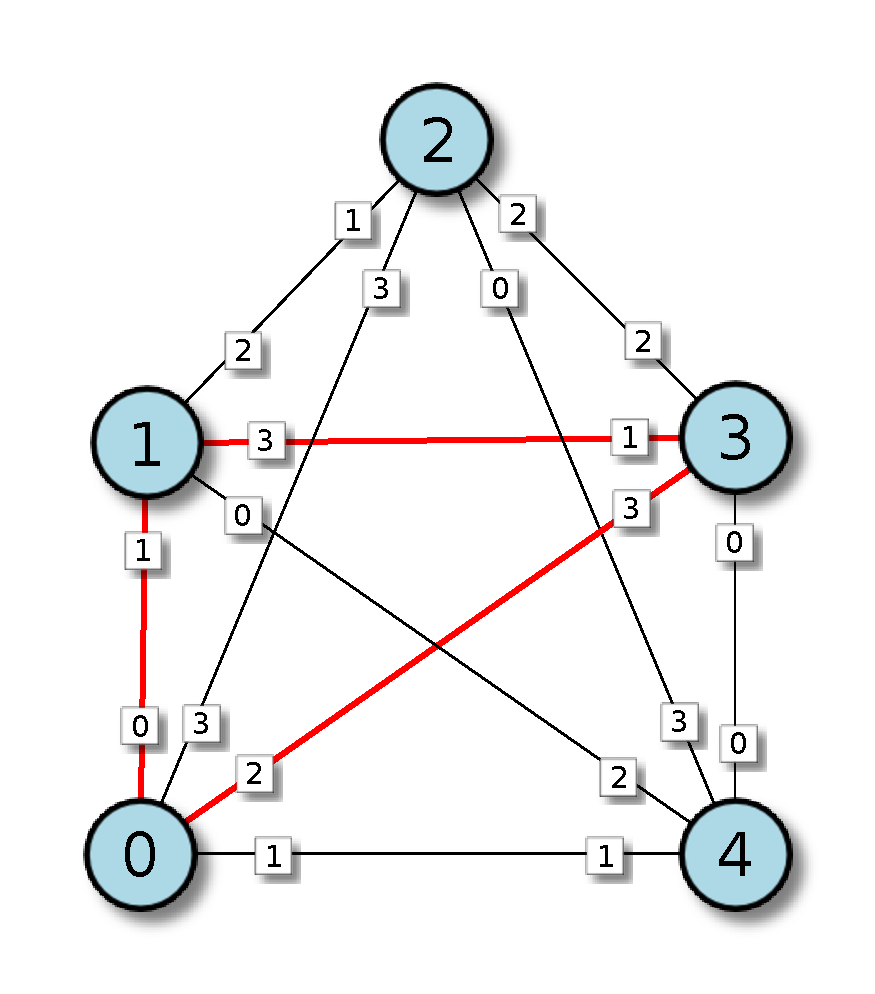
\includegraphics[height=.48\textheight]{../pics/3-pcircuit}
        \caption{Parity circuit of length $3$ }
        \label{fig:K5ppath}
      \end{figure}
    }
    \only<2->{
      \begin{figure}[h]
        \centering
        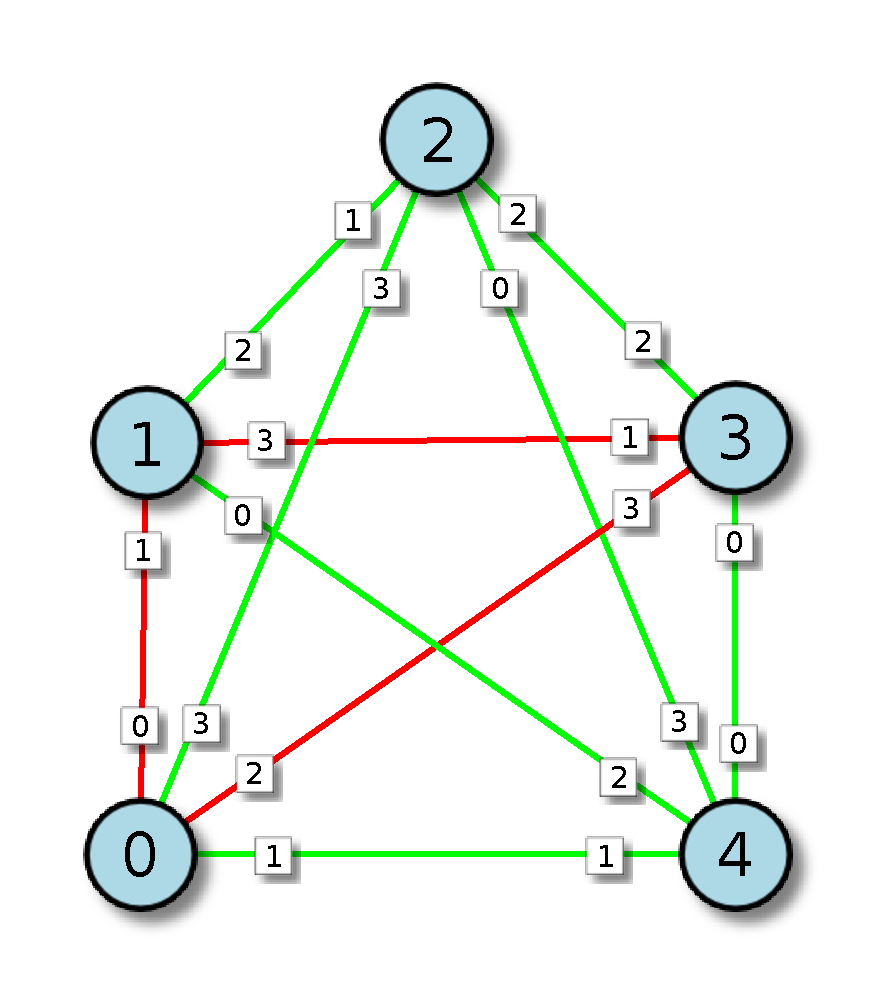
\includegraphics[height=.48\textheight]{../pics/37-pcd-example}
        \caption{Parity circuit of length $3$ }
        \label{fig:K5ppath}
      \end{figure}
    }
  \end{columns}
\end{frame}


\begin{frame}{Parity Circuit Decompositions (PCDs)}
  \begin{definition}
    \label{def:pcd}
    Sequence of parity circuits $\pcd = \left( \ppath_1, \ppath_2, \ldots, \ppath_j \right)$. is a  {\bf parity circuit decomposition (PCD)} of $K_5$ if 
    \begin{itemize}
      \item $\ppath_i$ and $\ppath_j$ are edgewise disjoint for $i \neq j$.
      \item For each $e \in \edgeS{K_5}$ there exists a parity circuit $\ppath_i$ such that $e$ is traversed by $\ppath_i$. 
    \end{itemize}
  \end{definition}
  \begin{columns}
    \column{.50\textwidth}
    \begin{figure}[h]
      \centering
      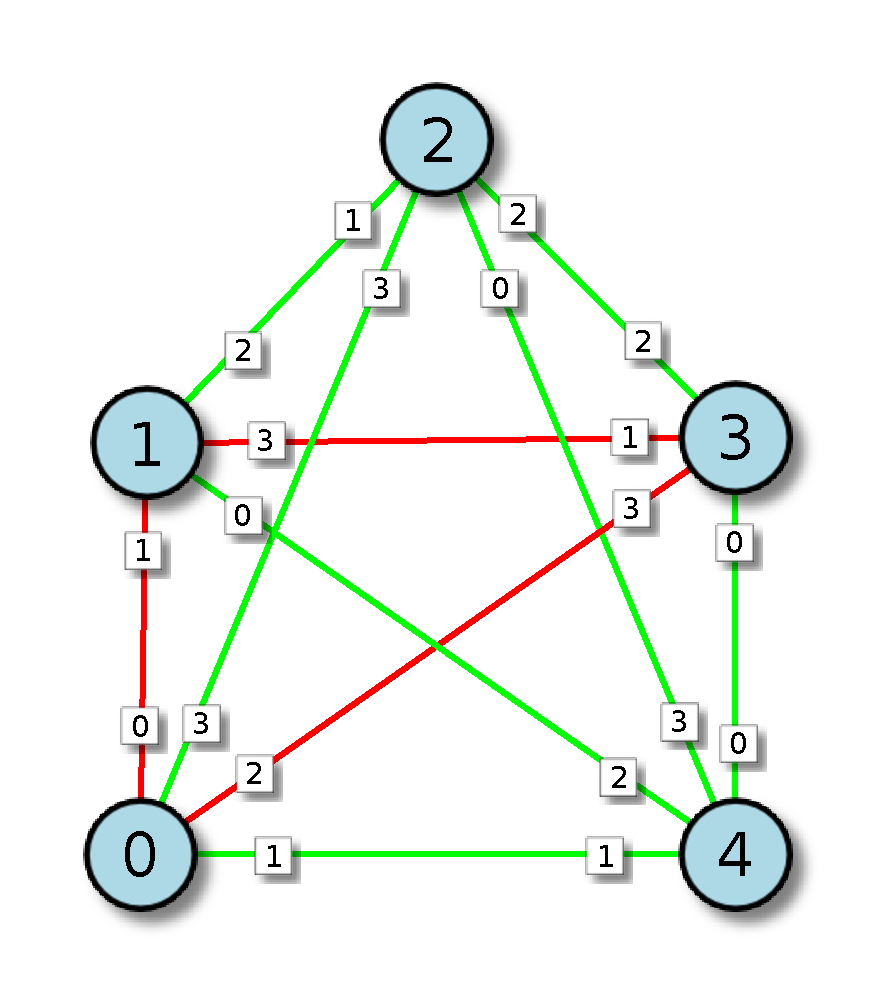
\includegraphics[height=.43\textheight]{../pics/37-pcd-example}
      \caption{Parity circuit decomposition of $K_5$}
      \label{fig:K5ppath}
    \end{figure}
    \column{.50\textwidth}
    \begin{itemize}
      \item $\pcd =$ \textcolor{red}{$\left[0 \ 1 \ 3 \right]$}\textcolor{green}{$\left[0\ 2\ 1\ 4\ 3\ 2\ 4 \right]$}
    \end{itemize}
  \end{columns}
\end{frame}
\begin{frame}{PCDs and $K_5 \protect\zigzag C_4$}
  \begin{columns}
    \column{.50\textwidth}
    \begin{itemize}
    \item $\pcd =$ \textcolor{red}{$\left[0 \ 1 \ 3 \right]$}\textcolor{green}{$\left[0\ 2\ 1\ 4\ 3\ 2\ 4 \right]$}
    \end{itemize}
    \begin{figure}[h]
      \centering
      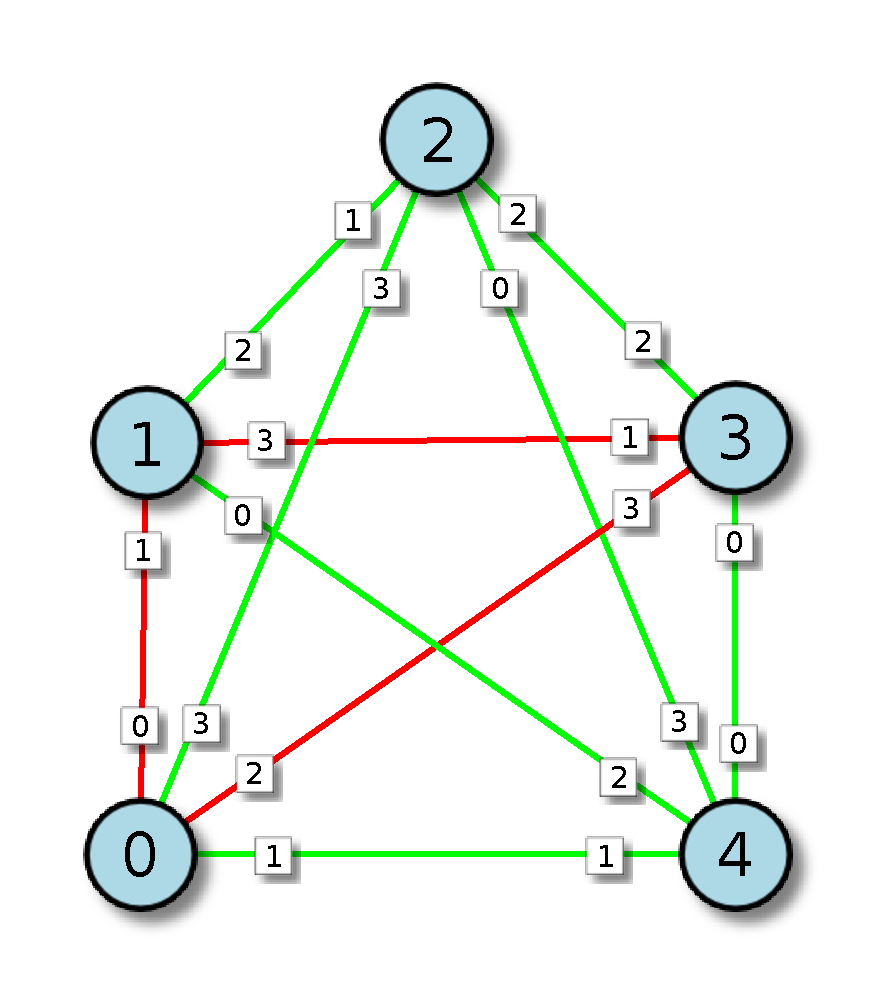
\includegraphics[height=.43\textheight]{../pics/37-pcd-example}
      \caption{Parity circuit decomposition of $K_5$}
      \label{fig:K5ppath}
    \end{figure}
    \column{.50\textwidth}
        \begin{figure}[h]
      \centering
      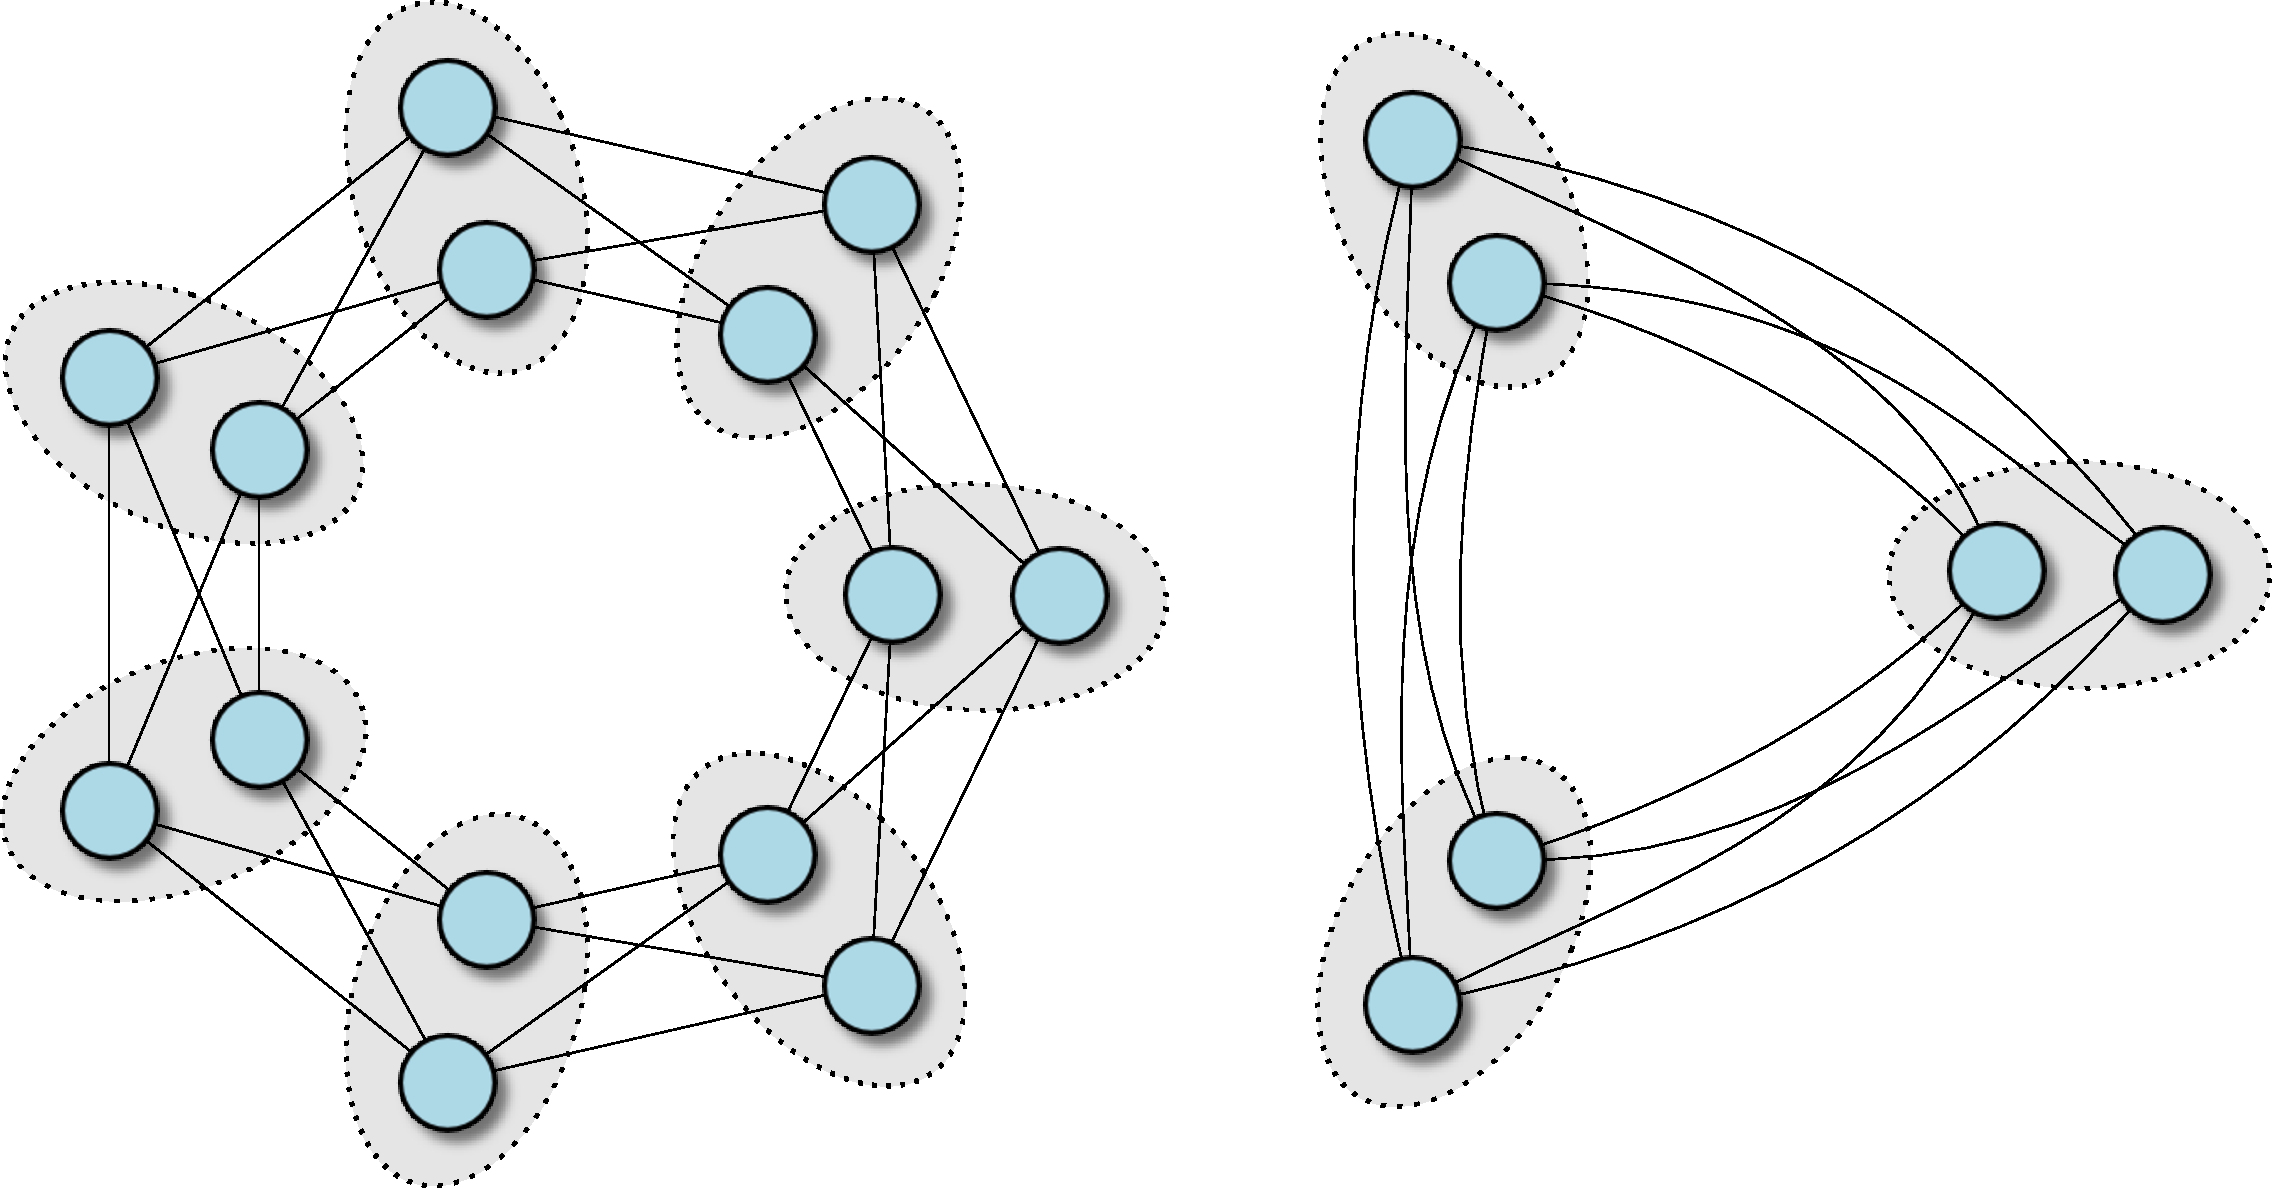
\includegraphics[height=.30\textheight]{../pics/3-7-zigzag}
      \caption{$K_5 \protect\zigzag C_4$}
    \end{figure}
  \end{columns}
\end{frame}
\begin{frame}{Equivalence of PCDs and uniqueness}

  \begin{itemize}
  \item $\ppath \equiv \ppath^{\prime}$ if $\ppath = \acts{\left(r \circ c_{i}\right)}{\ppath^{\prime}}$ where $r$ is a reversal of order and $c$ is a cyclic shift of length $i$.
  \item $\pcd \equiv \pcd^{\prime}$ if each parity circuit of $\pcd$ is equivalent to exactly one parity circuit in $\pcd^{\prime}$. 
  \end{itemize}
  
  \begin{example}
    \[ \left[0\ 1\ 3 \right]\left[0\ 2\ 1\ 4\ 3\ 2\ 4 \right] \equiv \left[3\ 0 \ 1\right]\left[4\ 1\ 2\ 0\ 4\ 2\ 3\right] \equiv \left[1\ 0\ 3\right]\left[1\ 4\ 3\ 2\ 4\ 0\ 2\right]\]
\[    \left[0\ 1\ 3 \right]\left[0\ 2\ 1\ 4\ 3\ 2\ 4 \right] \not\equiv \left[3\ 1\ 4\right]\left[3\ 0\ 4\ 2\ 0\ 1\ 2\right] \]
  \end{example}
  \uncover<2->{{\bf Note:} PCDs are equivalent if the pc's traverse the same edges}
\end{frame}

\begin{frame}{Facts about PCDs}

  \begin{itemize}
     \item<1-> Up to the equivalence discussed, every $\Enum$ determines a unique $\pcd_{\Enum}$
     \item<2-> Every vertex appears exactly two times in $\pcd$
     \item<3-> The smallest parity circuit is of length $3$
     \item<4->  The lengths of the parity circuits add up to $10$.  
  \end{itemize}
  \begin{columns}
    \column{.50\textwidth}
    \begin{figure}[h]
      \centering
      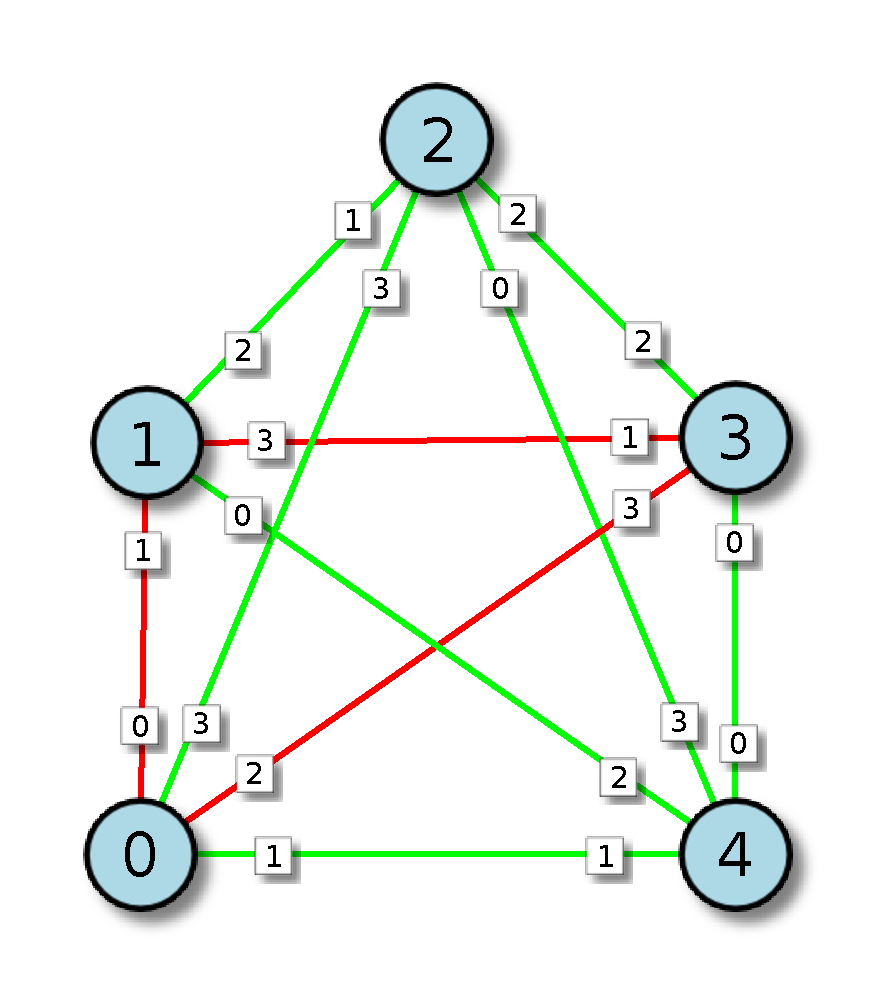
\includegraphics[height=.43\textheight]{../pics/37-pcd-example}
      \caption{$\pcd =$ \textcolor{red}{$\left[0 \ 1\ 3 \right]$}\textcolor{green}{$\left[0\ 2\ 1\ 4\ 3\ 2\ 4 \right]$}}
    \end{figure}
    \column{.50\textwidth}
    \begin{figure}[h]
      \centering
      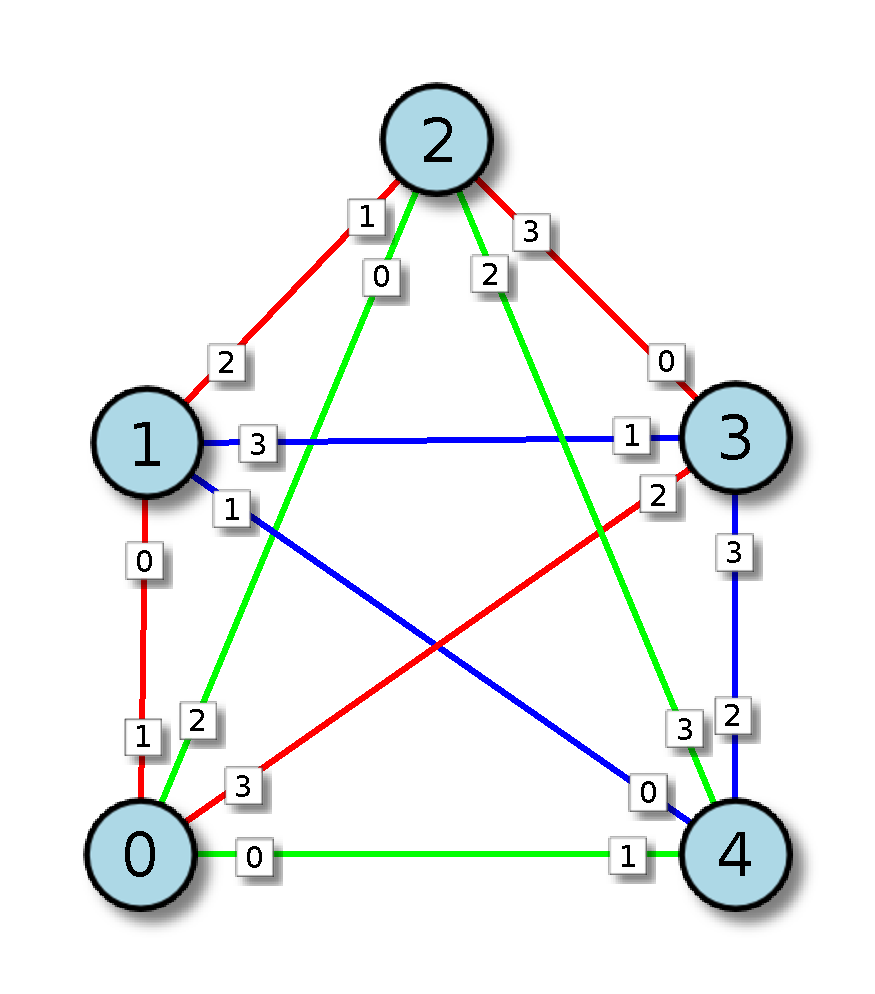
\includegraphics[height=.43\textheight]{../pics/334-pcd-example}
      \caption{$\pcd =$ \textcolor{red}{$\left[0 \ 1 \ 3 \right]$}\textcolor{green}{$\left[0\ 2\ 4\right]$}\textcolor{blue}{$\left[1\ 3\ 4 \right]$}}
    \end{figure}
  \end{columns}
\end{frame}

\begin{frame}{Signature of a PCD}
\begin{definition}
  \label{def:signature}
Let $\pcd = \left\{ \ppath_1 , \ldots, \ppath_k \right\}$ be a parity circuit decomposition of $K_5$. The list of lengths of each circuit, ordered by size, is called the {\bf signature} of the PCD. 
\end{definition}
  \begin{columns}
    \column{.50\textwidth}
    \begin{figure}[h]
      \centering
      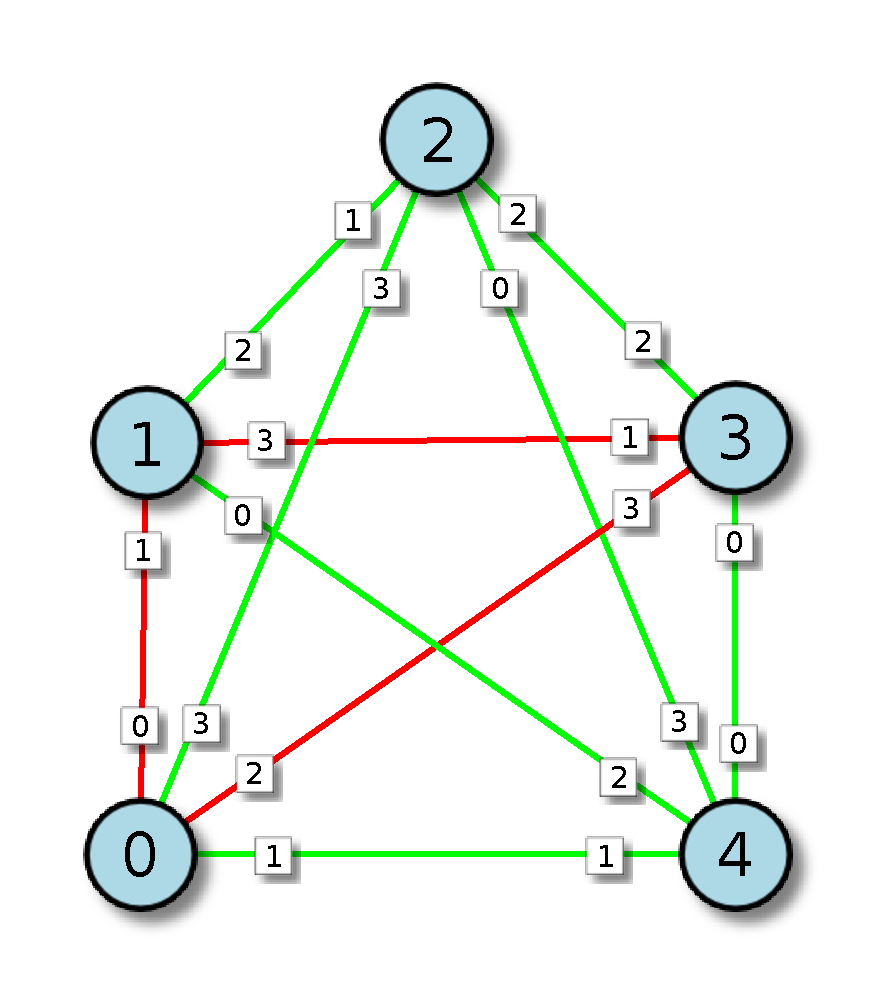
\includegraphics[height=.43\textheight]{../pics/37-pcd-example}
      \caption{Example of $3,7$-pcd}
    \end{figure}
    \column{.50\textwidth}
    \begin{figure}[h]
      \centering
      \includegraphics[height=.43\textheight]{../pics/334-pcd-example}
      \caption{Example of a $3,3,4$-pcd}
    \end{figure}
  \end{columns}
\end{frame}

\begin{frame}{Facts about the signature}
\begin{theorem}
  \label{thm:K_5partition10}
The signature of a parity circuit decomposition $\pcd$ is a partition of $10$ with terms no smaller than $3$. Which implies that the signature of any enumeration is equal to one of the following
 \begin{itemize}
 \item $3,3,4$.
 \item $3,7$.
 \item $4,6$.
 \item $5,5$.
 \item $10$.
 \end{itemize}
\end{theorem}
\end{frame}

\section{Counting  PCDs}

\begin{frame}{The number of unique PCD's}
\begin{block}{}
  \begin{itemize}
  \item Taken up to the equivalence that we spoke of earlier, we are interested in counting the number of unique PCDs. 
  \end{itemize}
\end{block}

\begin{theorem}
  \label{thm:pcd_count}
  The number of unique parity circuit decompositions is $3^5$
\end{theorem}

\begin{columns}
  \column{.50\textwidth}
  \begin{figure}[h]
    \centering
    \includegraphics[height=.35\textheight]{../pics/37-pcd-example}
    \caption{Example of $3,7$-pcd}
  \end{figure}
  \column{.50\textwidth}
  \begin{figure}[h]
    \centering
    \includegraphics[height=.35\textheight]{../pics/334-pcd-example}
    \caption{Example of a $3,3,4$-pcd}
  \end{figure}
\end{columns}
\end{frame}

\begin{frame}{Sketch of Proof}
Let:
\begin{itemize}
  \item<2->  $\EnumSet$ be the set of all enumerations of $K_5$
  \item<3->  $\pcdSet$ be the set of all parity circuit decompositions (modulo equivalence)
  \item<4->  $F:\EnumSet \mapsto \pcdSet $ be the natural mapping that sends an enumeration $\Enum$ to $\pcd_{\Enum}$
  \item<5-> Let $D_4 = \left< \left(0\ 1\ 2\ 3\right), \left( 0\ 2 \right)\left(1\ 3\right) \right>$(Dihedral Group)
\end{itemize}

\begin{block}{}
  \begin{itemize}
  \item<6-> We will use $F$ to define a bijection that will allow for us to count the number of unique PCDs.
  \end{itemize}
\end{block}
\end{frame}



\begin{frame}{Sketch of Proof}

\begin{lemma}
\label{lem:coset_lemma}
$F(\acts{\sigma}{\Enum}) = F(\acts{\pi}{\Enum})$ if and only if $\sigma^{-1} \circ \pi \in D_{4}^{5}$
\end{lemma}
\begin{columns}
  \column{.50\textwidth}
  \begin{figure}[h]
      \centering
      \includegraphics[height=.43\textheight]{../pics/334-pcd-example}
      \caption{Example of a $3,3,4$-pcd}
    \end{figure}
  \column{.50\textwidth}
  \begin{figure}[h]
      \centering
      \includegraphics[width=.80\textwidth]{../pics/334-pcd-example-replacement}
      \caption{$K_5 \protect\replacement C_4$}
    \end{figure}
\end{columns}

\end{frame}

\begin{frame}{Sketch of Proof}
\begin{theorem}
  \label{thm:cosets_bijection}
Let $\Enum^{0} \in \EnumSet$ and let $F^{*}:S_{4}^5 / D_{4}^5 \mapsto \pcdSet$ given by $\sigma D_{4}^5 \mapsto F\left( \acts{\sigma}{\Enum^{0}}\right)$. Then $F^{*}$ is a bijection.  
\end{theorem}

\begin{proof}
Since $F(\acts{\sigma}{\Enum}) = F(\acts{\pi}{\Enum})$ iff $\sigma^{-1} \circ \pi \in D_{4}^{5}$ we have that $F^{*}$ is an injection of the cosets of $S_{4}^5 / D_{4}^5$ and the mapping is surjective by definition. 
\end{proof}

\end{frame}

\begin{frame}{Sketch of Proof}
\begin{corollary}
  \label{cor:cardP_cosets}
   $\card{\pcdSet} = \left[ S_{4}^5 \ : \ D_{4}^{5}\right]$
\end{corollary}

\begin{block}{}
 Lagrange's Theorem gives us that  \[  \card{\pcdSet} = \left[ S_{4}^5 \ : \ D_{4}^{5}\right] = \frac{(4!)^5}{(8)^5} = 3^5  \]
\end{block}
\end{frame}

\section{Classifying  PCDs}

\begin{frame}{Classifying PCDs}
  \begin{itemize}
    \item<1-> Next we will seek to classify the $3^5$ parity circuit decompositions discussed earlier.
    \item<2-> We will do this by examining how the natural group action provided by $S_5$ on the vertices of $K_5$ affects the circuit decomposition.
  \end{itemize}


\end{frame}

\begin{frame}{How $S_5$ acts on a $\pcd$}
\begin{example}
 If $\sigma_1 = \left(0\ 1\ 3\ 4\right)\left(2\right)$ then 
  \[ \acts{\sigma_1}{\left[0\ 1\ 3\right]\left[0\ 2\ 1\ 4\ 3\ 2\ 4\right]} = \left[1\ 3\ 4\right]\left[1\ 2\ 3\ 0\ 4\ 2\ 0\right] \]
\end{example}
\begin{example}
If $\sigma_2 = \left(0\ 3\right)\left(2\ 4\right)\left(1\right)$ then
\[   \acts{\sigma_1}{\left[0\ 1\ 3\right]\left[0\ 2\ 1\ 4\ 3\ 2\ 4\right]} = \left[3\ 1\ 0\right]\left[3\ 4\ 1\ 2\ 0\ 4\ 2\right]  \]
\end{example}
\uncover<2->{{\bf Note:} $\sigma_2$ fixes the PCD (modulo equivalence).}
\end{frame}

\begin{frame}{Counting Using the Orbit Stabilizer Theorem}

The orbit-stabilizer theorem relates the cardinality of the orbit of an element under a group action to both the size of the group and it's stabilizer.
 \[ \card{\orbit{G}{s}} = \frac{\card{G}}{\card{\stab{G}{s}}}   \]

\end{frame}


\begin{frame}{Summary of Classification}
\begin{table}[h]
\caption{Summary of PCDs with given signature}
\label{tbl:summary}
\centering
\begin{tabular}[h]{|c|c|c|}
\hline
 Signature (Type) &  Representative PCD & Size of Orbit  \\
\hline
3,3,4 & $\left[0\ 1 \ 2\ 3 \right]\left[0\ 2\ 4 \right]\left[1\ 3\ 4\right]$ & $\frac{5!}{8} = 15$ \\
\hline
3,7 &$\left[0\ 1\  2 \right]\left[0\ 3\ 4\ 2\ 3\ 1\ 4 \right] $& $\frac{5!}{2} = 60$ \\
\hline
4,6 & $\left[0\ 1\ 2\ 3   \right]\left[0\ 4\ 3\ 1\ 4\ 2 \right]$   & $\frac{5!}{4} = 30$\\
\hline
5,5 & $\left[0\ 1\ 2\ 3\ 4 \right] \left[0\ 2\ 4\ 1\ 3 \right]$  & $\frac{5!}{20} = 6 $ \\ 
\hline
$10$ ($4$-distinct) &$\left[0\ 1\ 2\ 3\ 1\ 4\ 3\ 0\ 4\ 2  \right]$   &$\frac{5!}{10} = 12$ \\
\hline
$10$ ($5$-distinct/4 start) & $\left[0\ 1\ 2\ 3\ 4\ 1\ 3\ 0\ 4\ 2\right]$   &$\frac{5!}{2} = 60 $ \\
\hline
$10$ ($5$-distinct/8 start) & $\left[0\ 1\ 2\ 3\ 4\ 2\ 0\ 3\ 1\ 4  \right]$ & $\frac{5!}{2} = 60$ \\
\hline
Total & &  $3^5 = 243$ \\
\hline
\end{tabular}
\end{table}
\end{frame}

\begin{frame}{}
\begin{table}[h]
\caption{Summary of PCDs with given signature and their stabilizing group}
\label{tbl:summary}
\centering
\begin{tabular}[h]{|c|c|}
\hline
 Representative PCD & Stabilizing Group \\
\hline
 $\left[0\ 1 \ 2\ 3 \right]\left[0\ 2\ 4 \right]\left[1\ 3\ 4\right]$& $\left<\  (0\ 1\ 2\ 3)(4),\  (1\ 2)(0\ 3)(4)\  \right>$\\
\hline
$\left[0\ 1\  2 \right]\left[0\ 3\ 4\ 2\ 3\ 1\ 4 \right]$ & $\left<\ (0\ 2)(3\ 4)(1)\  \right>$ \\
\hline
$\left[0\ 1\ 2\ 3   \right]\left[0\ 4\ 3\ 1\ 4\ 2 \right]$  & $\left<\  (0\ 1\ 2\ 3)(4)\ \right>$ \\
\hline
$\left[0\ 1\ 2\ 3\ 4 \right] \left[0\ 2\ 4\ 1\ 3 \right]$  & $\left<\ (0\ 1\ 2\ 3\ 4),\ \left(0\right) \left(1\ 2\ 4\ 3\right)  \right>$ \\ 
\hline
$\left[0\ 1\ 2\ 3\ 1\ 4\ 3\ 0\ 4\ 2  \right]$&$\left<\left(0\ 2\ 1\ 3\ 4\right),\ \left(3\right)\left(0\ 2\right)\left(1\ 4\right)\right>$ \\
\hline
 $\left[0\ 1\ 2\ 3\ 4\ 1\ 3\ 0\ 4\ 2\right]$& $\left<\left(0\ 2\right)\left(1\ 4\right)\left(3\right) \right>$ \\
\hline
 $\left[0\ 1\ 2\ 3\ 4\ 2\ 0\ 3\ 1\ 4  \right]$&$\left<\ (0\ 3)(1\ 1)(4)\  \right>$ \\
\hline
\end{tabular}
\end{table}
\end{frame}

\begin{frame}{Justification: PCDs with a 4-cycle}
  \begin{block}{}
\begin{center}
    $\stab{S_5}{\left[0\ 1 \ 2\ 3 \right]\left[0\ 2\ 4 \right]\left[1\ 3\ 4\right]} =  \left<\  (0\ 1\ 2\ 3)(4),\  (1\ 2)(0\ 3)(4)\  \right>$  \\  and \\  $\stab{S_5}{\left[0\ 1\ 2\ 3   \right]\left[0\ 4\ 3\ 1\ 4\ 2 \right]} = \left<\  (0\ 1\ 2\ 3)(4)\ \right> $
\end{center}
  \end{block}
  \begin{columns}
    \column{.50\textwidth}
    \begin{figure}[h]
      \centering
      \includegraphics[width=.60\textwidth]{../pics/K54cycle}
      \caption{Both PCD's have $4$-cycle. }
      \label{fig:4cycle}
    \end{figure}
    \column{.50\textwidth}
    \begin{figure}[h]
      \centering
      \includegraphics[width=.70\textwidth]{../pics/4cycleunwrapped}
      \caption{$K_5$ with $\left[0\ 1\ 2\ 3\right]$ removed }
      \label{fig:4cycle}
    \end{figure}
  \end{columns}
\end{frame}

\begin{frame}{Justification: $\left[0\ 1\  2 \right]\left[0\ 3\ 4\ 2\ 3\ 1\ 4 \right]$}
  \begin{block}{}
\begin{center}
    $\stab{S_5}{\left[0\ 1\  2 \right]\left[0\ 3\ 4\ 2\ 3\ 1\ 4 \right]} =  \left<\ (0\ 2)(3\ 4)(1)\  \right>$
\end{center}
  \end{block}
  \begin{columns}
    \column{.50\textwidth}
    \begin{figure}[h]
      \centering
      \includegraphics[width=.60\textwidth]{../pics/K53cycle}
      \caption{PCD with $3$-cycle. }
      \label{fig:4cycle}
    \end{figure}
    \column{.50\textwidth}
    \begin{figure}[h]
      \centering
      \includegraphics[width=.70\textwidth]{../pics/3cycleunwrapped}
      \caption{$K_5$ with $\left[0\ 1\ 2 \right]$ removed }
      \label{fig:4cycle}
    \end{figure}
  \end{columns}
\end{frame}

\begin{frame}{Justification: $\left[0\ 1\ 2\ 3\ 4 \right] \left[0\ 2\ 4\ 1\ 3 \right]$ }
  \begin{block}{}
\begin{center}
    $\stab{S_5}{\left[0\ 1\ 2\ 3\ 4 \right] \left[0\ 2\ 4\ 1\ 3 \right]} = \left<(0\ 1\ 2\ 3\ 4),\ \left(0\right) \left(1\ 2\ 4\ 3\right)\right>$
\end{center}
  \end{block}
  \begin{columns}
    \column{.50\textwidth}
    \begin{figure}[h]
      \centering
      \includegraphics[width=.60\textwidth]{../pics/K55cycle}
      \caption{PCD with $5$-cycle. }
      \label{fig:4cycle}
    \end{figure}
    \column{.50\textwidth}
    \begin{figure}[h]
      \centering
      \includegraphics[width=.70\textwidth]{../pics/5cycleunwrapped}
      \caption{$K_5$ with $\left[0\ 1\ 2\ 3\ 4 \right]$ removed }
    \end{figure}
  \end{columns}
\end{frame}
\begin{frame}{PCD's with 10 as a signature}
  \begin{block}{}
    Each of the prior classes have one representative per signature. PCD's with 10 as the signature have $3$ orbit representatives. 
  \end{block}
  \begin{itemize}
    \item  $\left[0\ 1\ 2\ 3\ 4\ 2\ 0\ 3\ 1\ 4  \right]$ (4 distinct)
    \item  $\left[0\ 1\ 2\ 3\ 4\ 1\ 3\ 0\ 4\ 2\right]$ (5 distinct, 4 start)
    \item  $\left[0\ 1\ 2\ 3\ 4\ 2\ 0\ 3\ 1\ 4  \right]$ (5 distinct, 8 start)
  \end{itemize}
\end{frame}

\begin{frame}{PCD's with 10 as a signature: Terminology }
  \begin{definition}
We will say that a PCD is {\bf  $n$-distinct} if the maximum number of unique vertices traversed before duplicates is equal to $n$    
  \end{definition}


  \begin{definition}
    We will call the starting vertex of a distinct sequence when reading from left to right  a {\bf forward start}, denoted $\underline{i}$,  and if it is the beginning of a distinct sequence reading from right to left a {\bf backward start}, which we denote $\overline{i}$. 
  \end{definition}
\end{frame}

\begin{frame}{PCD's with 10 as a signature}
  \begin{block}{The $3$ orbit-representatives for PCDs with signature $10$.}
    \begin{itemize}
       \item $\left[\underline{0}\ \overline{1}\ \underline{2}\ \overline{3}\ \underline{1}\ \overline{4}\ \underline{3}\ \overline{0}\ \underline{4}\ \overline{2}  \right]$ (4-distinct)
       \item $\left[\underline{0}\ 1\ 2\ 3\ \overline{4}\ \underline{1}\ 3\ 0\ 4\ \overline{2}\right]$ (5 distinct, 4 start)
       \item $\left[\underline{0}\ 1\ 2\ \overline{3}\ \overline{\underline{4}}\ \underline{2}\ 0\ 3\ \overline{1}\ \overline{\underline{4}}\right]$ (5 distinct, 8 start)
   \end{itemize}
 \end{block}
 \begin{block}{}
   All of the stabilizing groups are calculated by observing that $S_5$ must send $n$-distinct elements to $n$-distinct elements.
 \end{block}
\end{frame}

\begin{frame}{}
\begin{table}[h]
\caption{Summary of PCDs with given signature and their stabilizing group}
\label{tbl:summary}
\centering
\begin{tabular}[h]{|c|c|}
\hline
 Representative PCD & Stabilizing Group \\
\hline
 $\left[0\ 1 \ 2\ 3 \right]\left[0\ 2\ 4 \right]\left[1\ 3\ 4\right]$& $\left<(0\ 1\ 2\ 3)(4), (1\ 2)(0\ 3)(4) \right>$\\
\hline
$\left[0\ 1\  2 \right]\left[0\ 3\ 4\ 2\ 3\ 1\ 4 \right]$ & $\left<(0\ 2)(3\ 4)(1)\right>$ \\
\hline
$\left[0\ 1\ 2\ 3\right]\left[0\ 4\ 3\ 1\ 4\ 2 \right]$  & $\left< (0\ 1\ 2\ 3)(4)\right>$ \\
\hline
$\left[0\ 1\ 2\ 3\ 4 \right] \left[0\ 2\ 4\ 1\ 3 \right]$  & $\left< (0\ 1\ 2\ 3\ 4), \left(0\right) \left(1\ 2\ 4\ 3\right)\right>$ \\ 
\hline
$\left[0\ 1\ 2\ 3\ 1\ 4\ 3\ 0\ 4\ 2  \right]$&$\left<\left(0\ 2\ 1\ 3\ 4\right),\ \left(3\right)\left(0\ 2\right)\left(1\ 4\right)\right>$ \\
\hline
 $\left[0\ 1\ 2\ 3\ 4\ 1\ 3\ 0\ 4\ 2\right]$& $\left<\left(0\ 2\right)\left(1\ 4\right)\left(3\right) \right>$ \\
\hline
 $\left[0\ 1\ 2\ 3\ 4\ 2\ 0\ 3\ 1\ 4  \right]$&$\left<\ (0\ 3)(1\ 1)(4)\  \right>$ \\
\hline
\end{tabular}
\end{table}
\end{frame}


\section{PCDs, $K_5 \protect\replacement C_4$ and $K_5 \protect\zigzag C_4$}

\begin{frame}{PCDs, $K_5 \protect\replacement C_4$ and $K_5 \protect\zigzag C_4$}
  \begin{figure}[h]
    \centering
     \includegraphics[width=.80\textwidth]{../pics/10-example}
    \caption{An enumeration on $K_5$ with associated replacement and zig-zag products. }
    \label{fig:allthree}
  \end{figure}
\end{frame}

\begin{frame}{PCDs and $K_5 \protect\replacement C_4$}
  \begin{corollary}
  \label{cor:pcd_rpiso}
If $F$ is a replacement product isomorphism. $\acts{F}{\pcd}$ is a $\Enum^{\prime}$-{parity circuit decomposition} whenever $\pcd$ is a $\Enum$-{parity circuit decomposition} 
\end{corollary}


\begin{itemize}
\item<2-> Shows that two enumerations generate rp-isomorphic replacement products iff they generate the same PCD on $K_5$
\item<3-> The characterization of equivalent PCD's also characterize replacement products.  
\end{itemize}
\end{frame}

\begin{frame}{PCDs and the Replacement Product} 
  \begin{figure}[h]
    \centering
    \includegraphics[height=.70\textheight]{../pics/replacement_summary}
    \caption{The $7$ classes of $K_5 \protect\replacement C_4$}
    \label{fig:replacement_summary}
  \end{figure}
\end{frame}

\begin{frame}{PCD's and the Zig-Zag Product: $2$-trellis}
\begin{definition}
  \label{def:trellis}
A {\bf $t$-trellis} over a cycle $C_n$ is a graph with $t \cdot n$ vertices, partitioned into $S_1,\ldots, S_n$, such that each $S_i$ has $t$ elements and each element of $S_i$ is connected to each element of $S_{i+1}$ and $S_{i-1}$ where $i$ is taken modulo $n$. 
\end{definition}

\begin{figure}[h]
  \centering
  \includegraphics[height=.40\textheight]{../pics/10-zigzag}
  \caption{A $2$-trellis over $C_{10}$}
  \label{fig:2trellis}
\end{figure}

\end{frame}

\begin{frame}{PCD's and the Zig-Zag Product}

\begin{theorem}
\label{thm:zzcorrespondence}
$\left[u_1\  \cdots\  u_k\right]$ is a parity circuit with parity $a_i$ at $u_i$ if and only if $K_5 \zigzag C_4$ has a subgraph that is a  $2$-trellis over $C_k$ with $S_i = \left\{ (u_i, 1-a_i), (u_i, 3-a_i)\right\}$ for $i =1,\ldots,k$.
\end{theorem}


\begin{theorem}
\label{thm:final_theorem}
Each connected component of $K_5 \zigzag C_4$ is a $2$-trellis over a cycle $C_j$.
\end{theorem}


\end{frame}

\begin{frame}
  \begin{block}{}
    Theorems demonstrate that there is a one-to-one correspondence between the PCDs of $K_5$ and the components of $K_5 \zigzag C_4$.
  \end{block}
  \begin{columns}
    \column{.50\textwidth}
    \begin{figure}[h]
      \centering
      \includegraphics[width=.80\textwidth]{../pics/37-pcd-example}
      \caption{$K_5$ with $3,7$-pcd}
      \label{fig:37-pcd}
    \end{figure}
    \column{.50\textwidth}
    \begin{figure}[h]
      \centering
      \includegraphics[width=.80\textwidth]{../pics/3-7-zigzag}
      \caption{$K_5 \protect\zigzag C_4$ with two components}
      \label{fig:37-zigzag}
    \end{figure}
  \end{columns}
\end{frame}

\begin{frame}{PCDs and the Zig-Zag Product}
  \begin{figure}[h]
    \centering
    \includegraphics[height=.75\textheight]{../pics/zigzag_summary}
    \caption{The $5$ classes of $K_5 \protect\replacement C_4$}
    \label{fig:replacement_summary}
  \end{figure}
\end{frame}



\part{Generalization of the Zig-Zag Product}
\begin{frame}{Generalization of the Zig-Zag Product}
    \begin{itemize}
    \item Finally we would like to define a zig-zag like product in a more general setting.
    \end{itemize}
  \begin{figure}[h]
    \centering
    \[
\xymatrix{ \edgeS{G} \ar@<-.5ex>[d]_{\Source_G} \ar@<+.5ex>[d]^{\Term_G} \\ \vertS{G} } \quad  \xymatrix{ \edgeS{G} \ar@(ul,ur)^{\Rot_G} \ar[d]^{\Source_G} \\ \vertS{G} }
\]
  \end{figure}
\end{frame}

\begin{frame}{Generalization of the Zig-Zag Product}

  \begin{itemize}
    \item<1-> We use a very general definition of graph and digraph.(Similar to Harary~\cite{Harary:1966}, {Mac Lane}~\cite{Lane:1971ys}, and Serre~\cite{Serre:1980})
    \item<2-> Introduce the {\em concatenation} and the {\em sandwich product} of graphs.
    \item<3-> Demonstrate that the zig-zag product of graphs may be concisely presented as the sandwich product of two relatively simple graphs.
  \end{itemize}
\end{frame}

\section{A New (and old) way to define a graph}

\begin{frame}{A New (and old) way to define a graph}
  \begin{definition}
\label{def:digraph}
A {\bf directed graph} (or {\bf digraph}), denoted by the letter $G$, is a collection of two sets $\edgeG$ and $\vertG$ together with two functions $\Source_G$ and $\Term_G$ from $\edgeG$ to $\vertG$ where  
\begin{itemize}
\item $\edgeG$ and $\vertG$ are known as the {\bf edge} and {\bf vertex} sets of the digraph $G$.
\item $\Source_G$ and $\Term_G$ are known as the {\bf source} and {\bf terminus} functions of the digraph $G$.
\[
\xymatrix{ \edgeS{G} \ar@<-.5ex>[d]_{\Source_G} \ar@<+.5ex>[d]^{\Term_G} \\ \vertS{G} }
\]
\end{itemize}
\end{definition}

\end{frame}

\begin{frame}{A New (and old) way to define a graph}

\begin{definition} 
An \textbf{undirected graph}, or just \textbf{graph},  is a digraph $G$ in which there exists a unique involution $\Rot_{G}:E \mapsto E$ such that $\Term_G = \sigma_G \circ \Rot_G$. We call the function $\Rot_G$ the {\bf rotation mapping} of the graph $G$.

\[
 \xymatrix{ \edgeS{G} \ar@(ul,ur)^{\Rot_G} \ar[d]^{\Source_G} \\ \vertS{G} }
\]

\end{definition}
\end{frame}

\section{The Sandwich Product}

\begin{frame}
\begin{definition}
\label{definition:pullback:set}
Let $A$, $B$, and $C$ be sets and let $f:A \mapsto C$ and $g:B \mapsto C$ be functions. Then the {\bf pullback} of set  functions $f$ and $g$ is the set \[ A \times_{C} B = \left\{  \left( a, b \right) \in A \times B\  \vert\  f\left(a\right) = g\left(b\right) \right\}  \] together with the standard coordinate projections $\pi_{1}$ and $\pi_{2}$.
\[
\label{diag:pullback_square}
\xymatrix{ A \times_{C} B \ar[r]^-{\pi_1} \ar[d]_{\pi_2} & B \ar[d]^{g}\\
   A \ar[r]_{f} & C
}
\] 
\end{definition}
\end{frame}

\begin{frame}
\begin{definition}
Let $G$ and $H$ be directed graphs with a common vertex set $V$ and let $E(G) \times_{V} E(H)$ be the pullback of the mappings $\Term_{G}$ and $\Source_{H}$.  Then the \textbf{concatenation} of $G$ with $H$, denoted by $G \concat H$,  is the directed graph with vertex set $V$,
edge set $E(G) {\times_{V}} E(H)$ , source map $\Source = \Source_{G} \circ \pi_{1}$ and terminus map $\Term = \Term_{H} \circ \pi_2$ as depicted in the diagram 
\[
\xymatrix{
   & E(G) \times_{V} E(H) \ar@<-.25em>[dd]_{\Source} \ar@<+.25em>[dd]^{\Term} \ar[dr]^{\pi_2} \ar[dl]_{\pi_1} &  \\
 E(G) \ar[dr]_{\Source_G}  & &  E(H) \ar[dl]^{\Term_{H}}  \\
   & V & 
}
\]
\end{definition}
\end{frame}


\begin{frame}

\begin{figure}[h!]
\centering
\[
\begin{array}[h]{ccc}
  \includegraphics[scale=.40]{../pics/three_cycle} & \includegraphics[scale=.40]{../pics/line} & \includegraphics[scale=.40]{../pics/concatination}
\end{array}
\]
\caption{Three cycle, three chain (with indicated source and terminus labeling) and their concatenation.\label{figure:example:concatenation}}
\end{figure}
\end{frame}

\begin{frame}
\begin{definition}
Let $G$ and $H$ be graphs with common vertex set $V$. Then the {\bf sandwich product} of $G$ with $H$, denoted $G \sandwich H$, is the graph with vertex set $V$, edge set 
\[
\left\{ ( f,e,f^{\prime} ) \in F \times E \times F  \ \vert \ \Term_{H}\left(f \right) = \Source_{G}\left(e \right)  \ {\rm and} \ \Term_{G}\left(e \right) = \Source_{H}\left(f^{\prime} \right) \right\}
\] with source map which takes $(e,f,e^{\prime}) \mapsto (\Source_{G}(e) , \Source_{H}(f))$ and rotation map \[\Rot((f,e,f^{\prime})) = \left(\Rot_{H}(f) , \Rot_{G}(e) ,\Rot_{H}(f^{\prime})\right)\]  
\end{definition}
\end{frame}

\section{A Zig-Zag Sandwich}

\begin{frame}  
\begin{definition}
\label{def:graph:zig} 
Let $G$ and $H$ be graphs. The the \textbf{zig product} of $G$ with $H$, denoted $G \zig H$,  is the graph depicted in the diagram
\[ 
\xymatrix{
  {V(G) \times E(H)} \ar[d]_{id_{V(G)} \times \Source_{H}}  \ar@(ul,ur)^{id_{V(G)} \times \Rot_{H}}  \\
     {V(G) \times V(H)}
}
\]
\end{definition}


\end{frame}

\begin{frame}
  \begin{definition} 
    \label{def:symnet:zag}
Let $G$ and $H$ be graphs and let $\phi:\edgeS{G} \mapsto \vertS{H}$ be an onto mapping. The {\bf zag product} of $G$ and $H$, denoted $G \zag H$, is the graph with  vertex set $V(G) \times V(H)$, 
edge set $\edgeS{G \zag H} = \edgeS{G}$, source mapping $\Source_{\rm zag} = \Source_{g} \times \phi$ and rotation mapping $\Rot_{\rm zag} = \Rot_{G}$ as depicted the diagram 
\[
\xymatrix{
  {E(G)} \ar[d]_{\Source_{G} \times \phi} \ar@(ul,ur)^{\Rot_{G}}  \\
  V(G) \times V(H)
}
\]
\end{definition}
\end{frame}


\begin{frame}
  \begin{definition}
 \label{def:cat_zigzag}
Let $G$ and $H$ be graphs with $\phi:\edgeS{G} \mapsto \vertS{H}$. Then the {\bf zig-zag} product of $G$ with $H$, denoted $G \zigzag H$, is the graph with vertex set $V(G) \times V(H)$,  edge set
\[ E(G \zigzag H) = \left\{  \left( f, e, f^{\prime} \right) \ \vert \ \Term_H\left(f\right) = \phi\left(e\right)\ \textrm{and} \  \phi\left( \Rot\left(e \right)  \right) = \Source_{H}\left(f^{\prime}\right)  \right\}, \] source mapping given by $\Source\left( \left(f, e, f^{\prime}\right)\right) = \left( \Source_G \left(e \right), \Source_{H}\left( f \right) \right)$ and rotation mapping $\Rot$ given by  \[ \Rot(e,f,e^{\prime}) = \left( \Rot_{H}\left( f^{\prime} \right) , \Rot_{G} \left( e \right), \Rot_{H } \left( f \right) \right)  \]
\end{definition}

  \begin{theorem}
\[ G \zigzag H = \left( G \zag H \right) \sandwich \left( G \zig H \right)
                   \]
\label{thm:zigzagsandwich} 
\end{theorem}
\end{frame}

\part{Conclusion}

\begin{frame}{Further Topics of Study}

  \begin{itemize}
    \item<1-> The classification of $G \replacement C_4$ and $G \zigzag C_4$ for any $4$-regular graph
    \item<2->  The classification of $G \replacement C_n$ and $G \zigzag C_n$.
    \item<3-> The Sandwich Product and the generalization to non-regular graphs.
    \item<4-> The Zig-Zag Product and it’s connection with the semi-direct product of groups.
    \item<5-> The Zig-Zag Product and it’s connection with the semi-direct product of groups
  \end{itemize}
\end{frame}

\begin{frame}{The classification of $G \protect\replacement C_4$ and $G \protect\zigzag C_4$ for any $4$-regular graph}

We would like to extend the definitions and theorems contained in the thesis to 

\begin{itemize}
\item $G \protect\replacement C_4$ and $G \protect\zigzag C_4$ for any $4$-regular graph.
\end{itemize}

\begin{itemize}
\item little work needs to be done to extend the concepts as they almost depend completely on the properties of $C_4$
\item Though much is not known about how $\Aut(G)$ being more general affects the classes of PCDs
\item it is suspected that when $G$ has a small automorphism group there will likely be many classes of replacement and zig-zag products.
\end{itemize}


\end{frame}

\begin{frame}{The classification of $G \protect\replacement C_n$ and $G \protect\zigzag C_n$}
  \begin{itemize}
  \item The zig-zag product when taken over $C_4$ is always a $2$-trellis. (which has bad expansion)
    \item It is suspected that the zig-zag product over larger cycles will yield a richer class of graphs with possibly better expansion properties.
      \item Still simple enough that a full classification is practical.
  \end{itemize}
\end{frame}

\begin{frame}{The Sandwich Product and the generalization to non-regular graphs}
  \begin{itemize}
  \item We considered a graph just a collection of functions.
    \item  have opened up an intriguing and, some would say, elegant method for describing the zig-zag product in a more general setting.
      \item Today the definitions are too broad to be useful for analysis, but by placing additional restrictions on the function involved there is hope for further development.
  \end{itemize}
\end{frame}

\begin{frame}{The Zig-Zag Product and it’s connection with the semi-direct product of groups}

  \begin{itemize}
  \item  Alon {et al.}~\cite{Alon:2001xy} presented an interesting connection between the semi-direct product and the zig-zag product of graphs.
  \item That with suitably chosen generating sets, the Cayley graphs of the semi-direct product of two groups can be seen as the zig-zag product of the constituent Cayley graphs.
  \item let $G = \mathbb{Z}_5$ with Cayley generating set $S_G = \mathbb{Z}_5 \setminus \{0\}$ and $H = \mathbb{Z}_4$ with generating set $S_H = \{\pm1\}$, then we have Cayley graphs which mirror $K_5$ and $C_4$
  \item  Obvious questions are how does the structure of the groups effect the enumeration which would be generated by these Cayley graphs.
  \end{itemize}
\end{frame}

\begin{frame}{Conclusion}
  \begin{block}{}
So in conclusion, as with most mathematical work, we are left with as many questions as we have answers. The hope of the author is that this thesis will be seen as a good first step.
\end{block}
\ \\
\begin{center}
{\Huge {\bf Any Questions?}}
\end{center}

{\bf Copy of Presentation:} \url{http://dl.dropbox.com/u/1768136/defense.pdf }\\ \ \\
{\bf Copy of Thesis:} \url{http://dl.dropbox.com/u/1768136/thesis.pdf} \\ \ \\
\end{frame}


\part{References}
\frame[t]
{
\frametitle{References}

\bibliography{../thesis}{}
\bibliographystyle{plain}
}
\end{document}